
% CHAPTER 4

\chapter{SIMULATION ENVIRONMENT $\&$ RESULTS}
\label{chp:simulation}


\externaldocument{chapter1}
\externaldocument{chapter2}
\externaldocument{chapter3}
\externaldocument{chapter6}
\externaldocument{chapter5}






In this section, the simulation environment is illustrated and the results are analyzed and discussed in detail for the local positioning system design and formation control system design. Three different methods of formation control system which are presented in Section \ref{chp:Methodology} are evaluated and compared with each other. Simulations are handled in the environment of Gazebo simulator with a swarm of 50 agents which includes three different types of robots. We have determined the position beacon ratio as $\%$15, so we have 8 position beacons in our swarm. The main system frequency in which each agent propagates its state vector, calculates artificial forces and makes goal state assignments is determined as 2Hz. 
\newpage
\section{Simulation Environment}
Block diagram of the simulation environment is illustrated in Figure \ref{simulation_env_ref}.

\begin{figure}[H]
\caption{Simulation Environment} \label{simulation_env_ref}
\centering
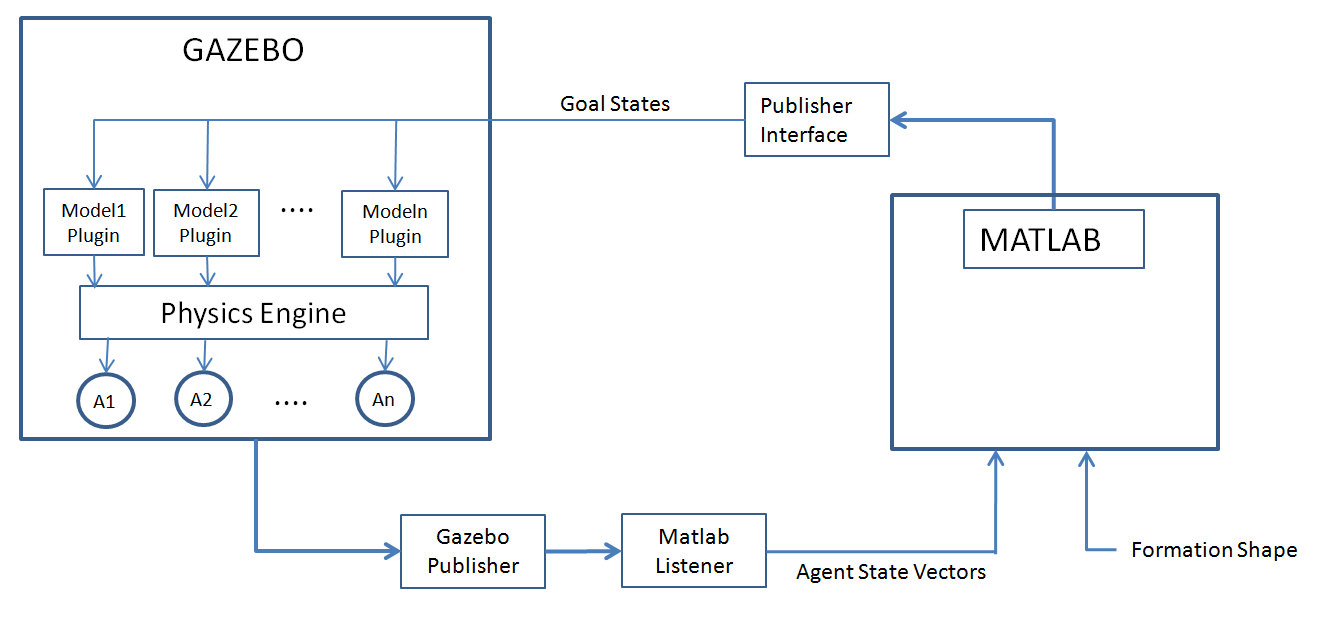
\includegraphics[scale = 0.45]{environment}
\end{figure}
    
Gazebo is an open source multi robot simulator developed by Open Source Robotics Foundation(OSRF). It has multiple physics engines; Open Dynamics Engine(ODE), Bullet, Dynamic Animation and Robotics Toolkit(DART) and Simbody. It can execute simulations with multiple agents in an environment that is fully created by the user. The dynamics and the physical properties of the robots are determined by the user. It can be integrated with Robot Operating System(ROS). We have used this simulator to run the dynamics of the agents with the help of ODE physics engine. We have created plugins dedicated on each agent to execute the algorithms in a decentralized topology as discussed in Section \ref{decent_decent}. Agents use these plugins to  listen goal states from Matlab environment, execute their decision process algorithms and calculate their artificial forces. These plugins also execute controller algorithms to make the agents reached to the goal states they have assigned.
 
Shape partitioning algorithms are executed in Matlab environment and goal states are published over a network socket. A plugin working in Gazebo environment, listens the packets sent by Matlab and parse the data for each agent type. The state vectors of the agents are published with a plugin from the Gazebo simulator and they are used to visualize the workpace in a Matlab plot. We have designed the workspace as a rough 3D territory and each agent have different interactions with the environment with different mass and friction characteristics. This workspace is defined with a square area with boundaries placed at +/-50 meters in x and y coordinates. We have assumed that the communication range of an agent is 25 meters. To simulate the radio link between any two agent, we use a line segment drawn between the centers of these agents' coverage circles. It is assumed that these two agents have a direct radio link (i.e. they are direct neighbors in the mesh network) if the $p_2$ norm of this vector is smaller than the communication range and this line segment doesn't intersect any workspace obstacles.

Figure \ref{Gazebo} illustrates the Gazebo simulation environment. 

\begin{figure}[H]
\caption{Simulation Environment in Gazebo} \label{Gazebo}
\centerline{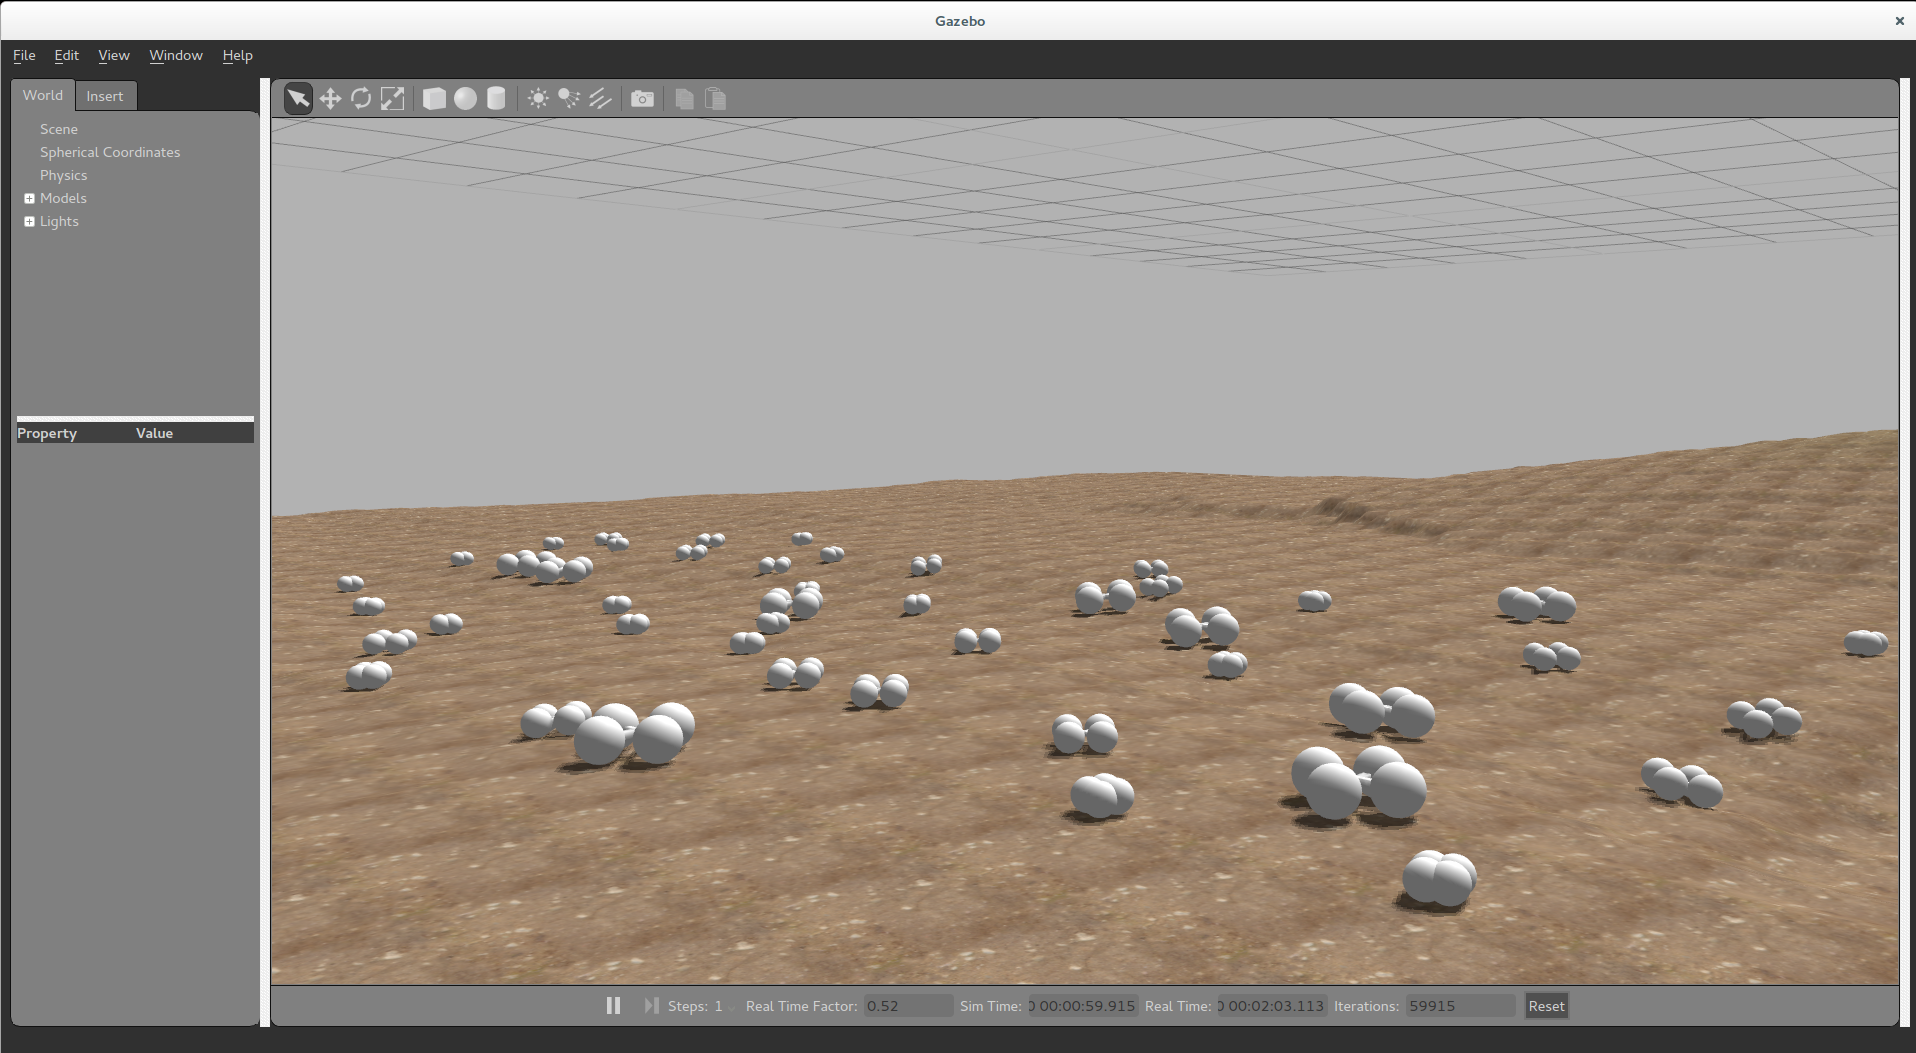
\includegraphics[scale = 0.22]{gazebo_env}}
\end{figure} 

In this simulation environment, each agent is designed with collision surfaces composed by four spheres which are assumed to have point interaction with the environment. Agents have cylindrical links binding these spherical contact points. The mass and friction coefficients for different types of agents are given in Table \ref{agent_props}. Here there are two different types of frictions, $\mu_1$ represents the dry friction coefficient and the $\mu_2$ is the fluid friction coefficient.

\begin{center}
\captionof{table}{Parameters for Different Types of Agents} \label{agent_props} 
\begin{tabular}{||c| c| c |c |c||}
				
\hline
\textbf{Agent Type} & \textbf{Mass[kg]}  & \textbf{$\mu_1$} & \textbf{$\mu_2$} & \textbf{Coverage Circle Radius[m]} \\ 
\hline
Agent 1& 0.8 & 0.21  & 0.13 & 0.15\\
Agent 2& 1   &  0.18 & 0.18 & 0.3\\	
Agent 3& 1.5 &  0.21 & 0.13 & 0.5\\	
\hline
\end{tabular}
\end{center}

As illustrated in Section \ref{lqr_design}, full state feedback gains for the agents are calculated with the help of LQR methodology by using the linear system definitions of different types of agents. Calculated feedback gains are given in Table \ref{feedback_gains}.

\begin{center}
\captionof{table}{State Feedback Gains for Different Types of Agents} \label{feedback_gains} 
\begin{tabular}{||c| c |c||}
				
\hline
\textbf{Agent Type} & \textbf{$K_e$}  & \textbf{$K_v$} \\ 
\hline
Agent 1& 237 & 96\\
Agent 2& 263 & 112\\
Agent 3& 297 & 121\\
\hline
\end{tabular}
\end{center}

Figure \ref{Matlab_env} illustrates the visualization of the workspace in the Matlab environment. Red circles which are the same size with coverage circles defined in Section \ref{Artificial_forces_ref}, are representing the different types of agents in the environment. The shape defined with blue line is the desired formation shape and the obstacles are represented with green lines in the environment. 

\begin{figure}[H]
\caption{Visualization of Workspace in Matlab} \label{Matlab_env}
\centerline{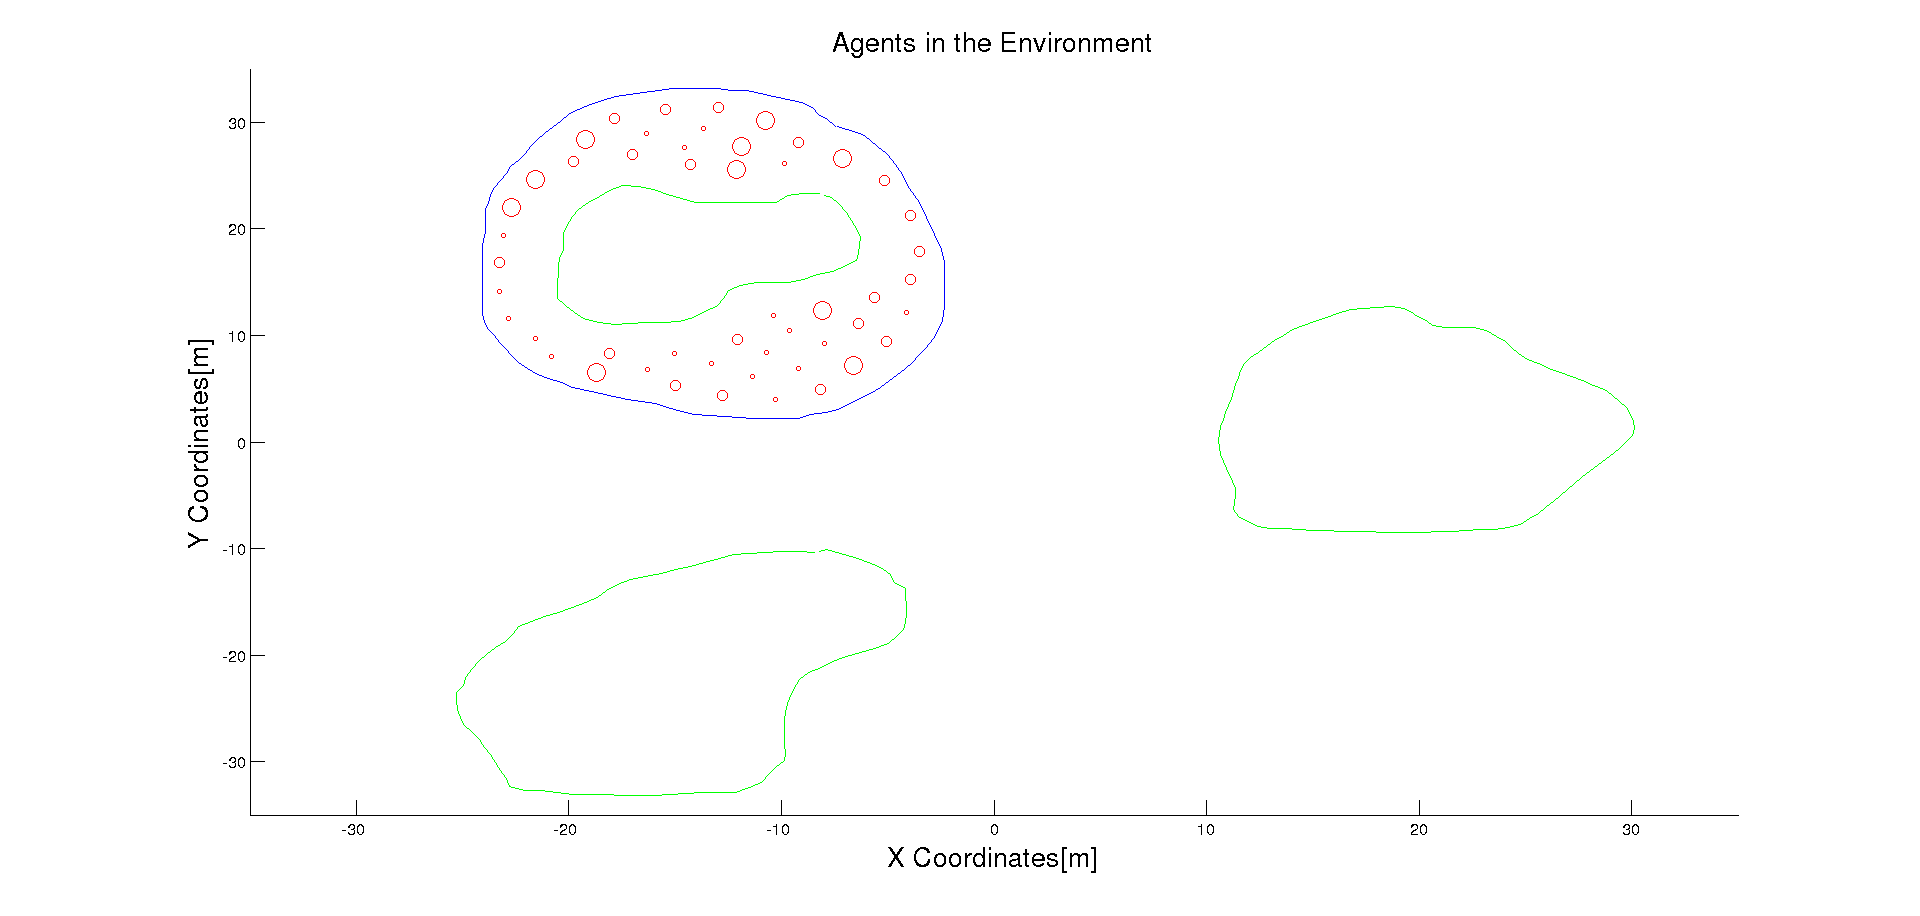
\includegraphics[scale = 0.30]{2}}
\end{figure} 
    
\section{Local Positioning System} \label{lps_ref}
In the local positioning system, the main aim is to design an architecture in which every second type agent can localize itself with the help of the position beacons. In this architecture, second type agents need external position measurements for their state estimator systems to prevent a potential drift in their position data. In our implementation, the state propagation frequency is determined as 2Hz which is equal to the main system frequency since the new position datas for the formation control system are required to be determined with this rate. 	As discussed in Section \ref{LOCAL POSITIONING SYSTEMS_ref}, a localization timer is proposed to provide the required minimum time to the DSDV algorithm and trilateration process.

We are expecting that the position data in the state vector will be drifting with the increasing time because of the errors and noise in inertial measurements unless they are not corrected with the external measurements \cite{91}. So it is possible to determine a minimum execution period of this trilateration process to satisfy a maximum error in the position data. For this purpose we have executed Monte Carlo simulations to observe the drift in the position data with state propagation process. In Figure \ref{3second_period}, \ref{5second_period} and \ref{8second_period}, the simulation outputs with different periods of localization timer are illustrated.
		
\begin{figure}[H]
\caption{Total Error with Localization Timer Period of 3 Seconds} \label{3second_period}
\centerline{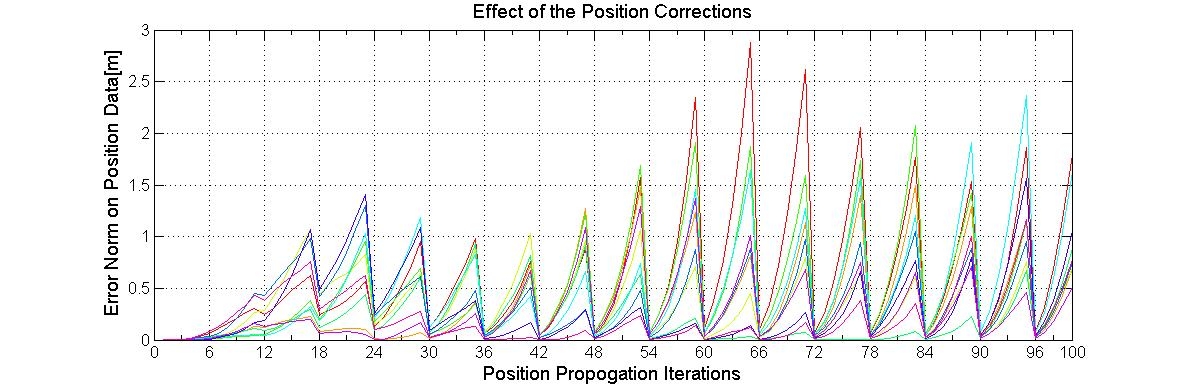
\includegraphics[scale = 0.4]{Error-0,5Prop-3Update}}
\end{figure} 
		
\begin{figure}[H]
\caption{Total Error with Localization Timer Period of 5 Seconds} \label{5second_period}
\centerline{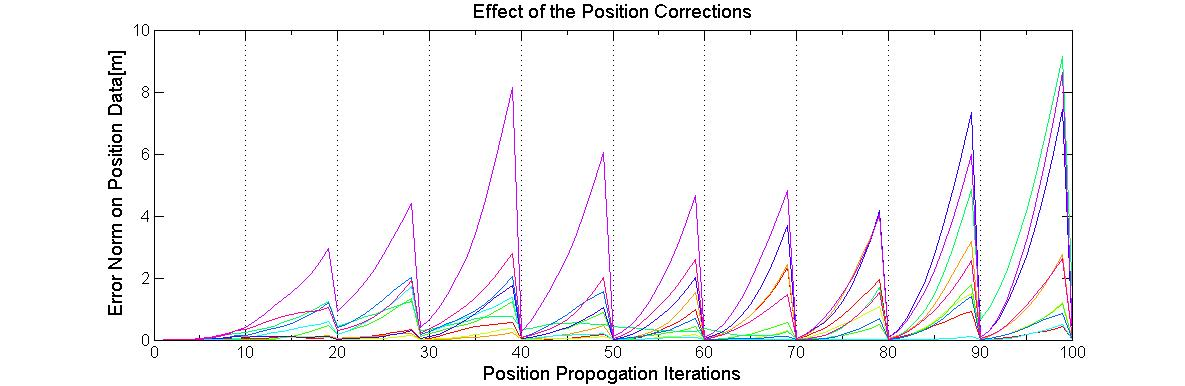
\includegraphics[scale = 0.4]{Error-0,5Prop-5Update}}
\end{figure} 

\begin{figure}[H]
\caption{Total Error with Localization Timer Period of 8 Seconds} \label{8second_period}
\centerline{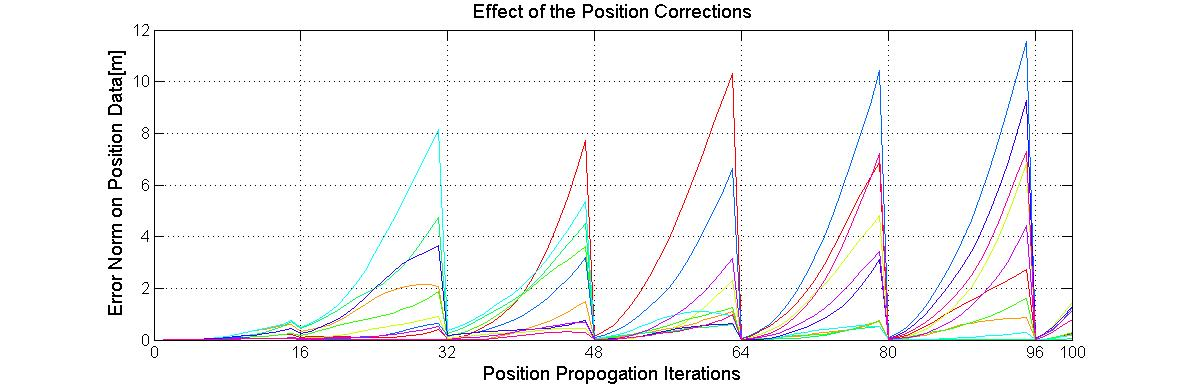
\includegraphics[scale = 0.4]{Error-0,5Prop-8Update}}
\end{figure} 		
		
According to these figures, it is clear that the total error norm on position datas are decreased dramatically with the localization period which equals to 6 iterations for 3 seconds period, 10 iterations for 5 seconds and 16 iterations for 8 seconds period. The peak values on the error norms are always observed at the iterations just before the localization process. It can be concluded that the peak values on the error norms are greatly related with the localization period and they have greater values with the increasing number of this period. The maximum error norm is below 3 meters with localization period of 3 seconds, below 10 meters with localization period of 5 seconds and below 12 meters with localization period of 8 seconds. In this work, it is assumed that the error norm of 3 meters is the maximum tolerable value for the formation control system to satisfy a successful collision avoidance for the agents since we have a coverage circle radius of 0.5m for the biggest agent in the swarm. Thus, the localization period for the trilateration process is determined as 3 seconds in simulations. 

The performance of the LPS design is tested in simulations with different conditions in which swarm is propagating to a desired formation shape or agents are keeping their positions in dynamically changing formation shapes.  In both cases, it is observed that the position datas of the agents are drifted with an increasing error between two  sequential localization process as we have discussed previously. A sample case for this situation is illustrated in Figure \ref{hatali_pos_ref} and Figure \ref{duzgun_pos_ref}. In these figures, red circles are representing the estimated positions of the agents where blue circles are representing the real positions. 

\begin{figure}[H]
\centering
\captionsetup{format=hang,justification=centerfirst}
\caption{Positions of the Agents Before Localization Process} \label{hatali_pos_ref}
\centerline{
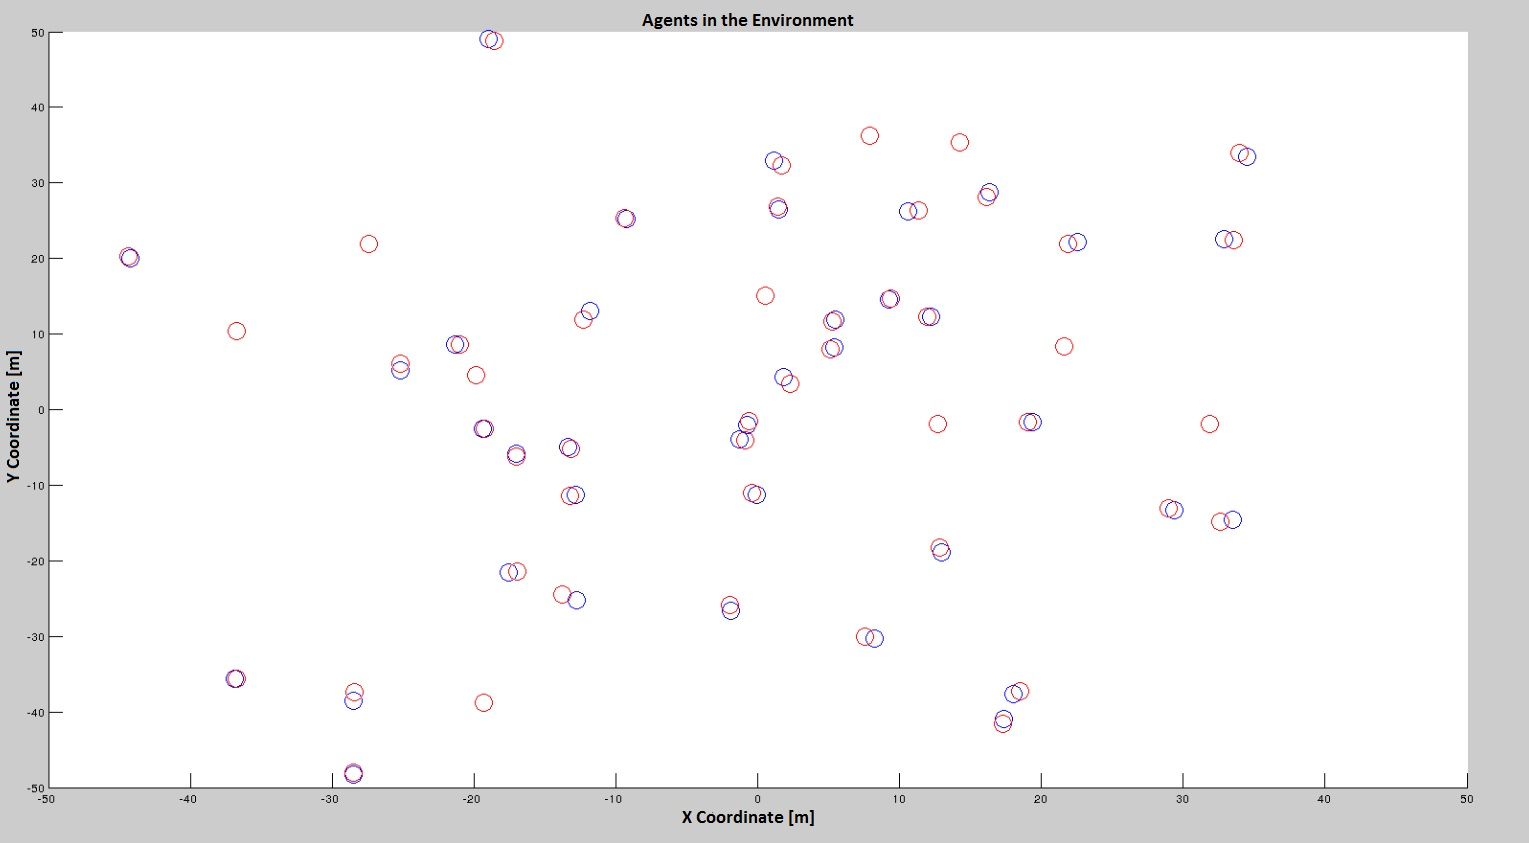
\includegraphics[scale = 0.35]{Pozisyon_1_Hatali}}
\label{fig:lps}
\end{figure}

\begin{figure}[H]
\centering
\captionsetup{format=hang,justification=centerfirst}
\caption{Positions of the Agents After Localization Process} \label{duzgun_pos_ref}
\centerline{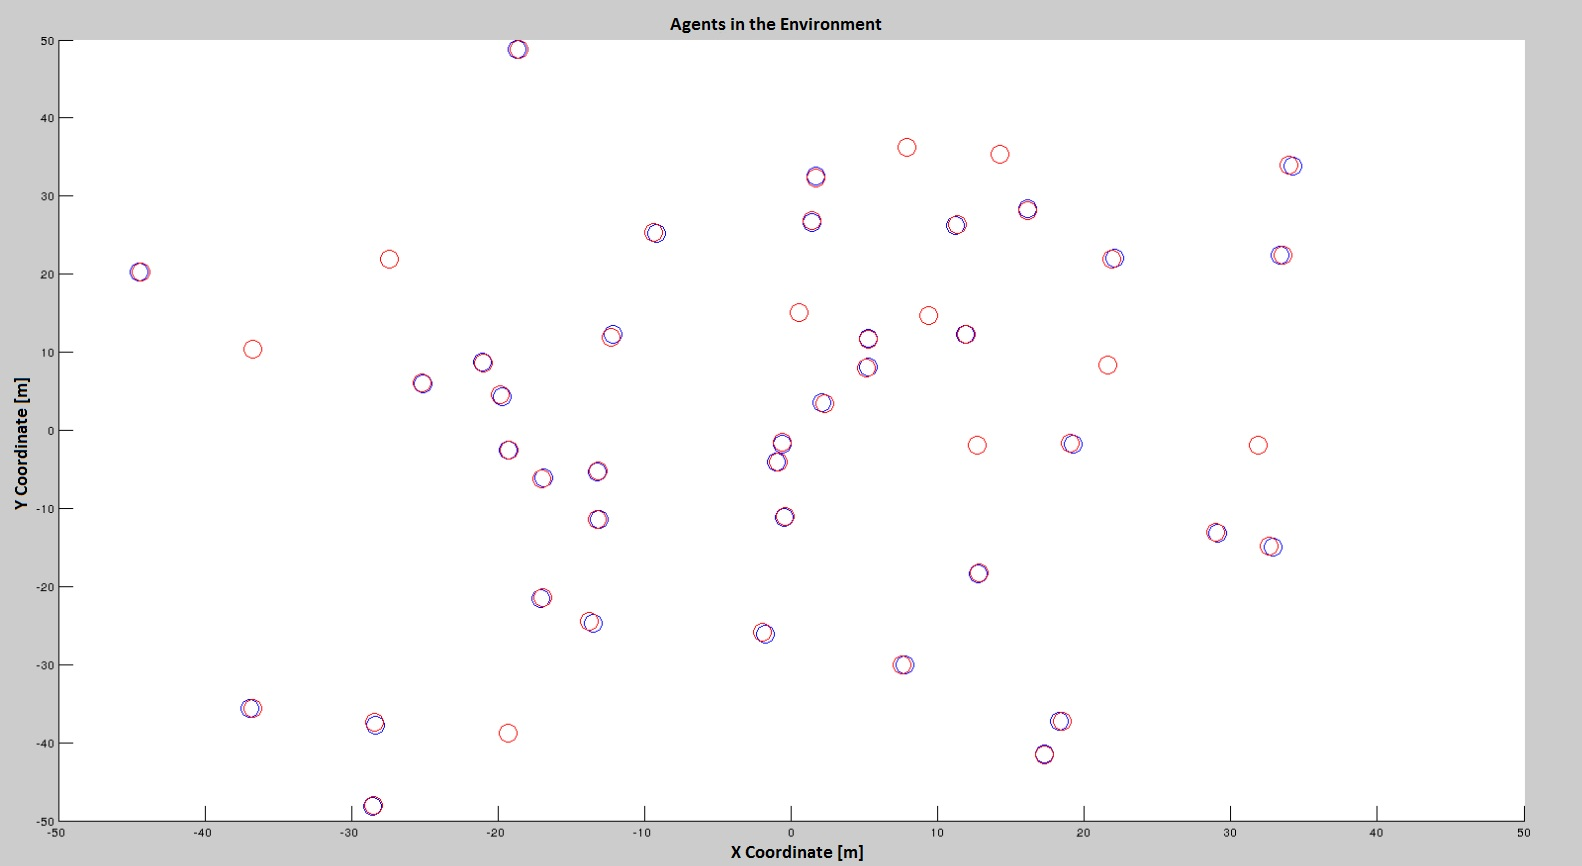
\includegraphics[scale = 0.25]{Pozisyon-1-Duzeltilmis}}
\end{figure} 
In Figure \ref{hatali_pos_ref}, blue and red circles do not coincide with each other. This shows us, there are errors on the estimated positions which are represented with red circles before the localization process. Figure \ref{duzgun_pos_ref} shows the workspace just after a localization process and it is possible to see that blue and red circles are getting close to each other with this process. This concludes that the error on the estimated position datas are reduced with the help of this process.
		
Handling procedures of the lost agents are presented in Section \ref{LostAgents}. Agents which do not have at least three position beacons which are direct neighbors around itselves will get into the 'Lost' mode, and if  they miss three localization process they will get into 'Come Home' mode. When an agent is in 'Come Home' mode, it will try to reach to the center of formation shape to increase the possibility of meeting some position beacons to localize itself. A simulation result in which two agents do not have three position beacons as direct neighbors around themselves is illustrated in following figures. They get into 'Lost' mode first, when they cannot find three position beacons as direct neighbors. After they miss three localization process, they get into 'Come Home' mode in which they are trying to reach to the center of formation shape.
		
\begin{figure}[H]
\caption{Agents will be in 'Lost' Mode When They Do Not Have 3 Neighbors} \label{lost_ref}
\centering
\centerline{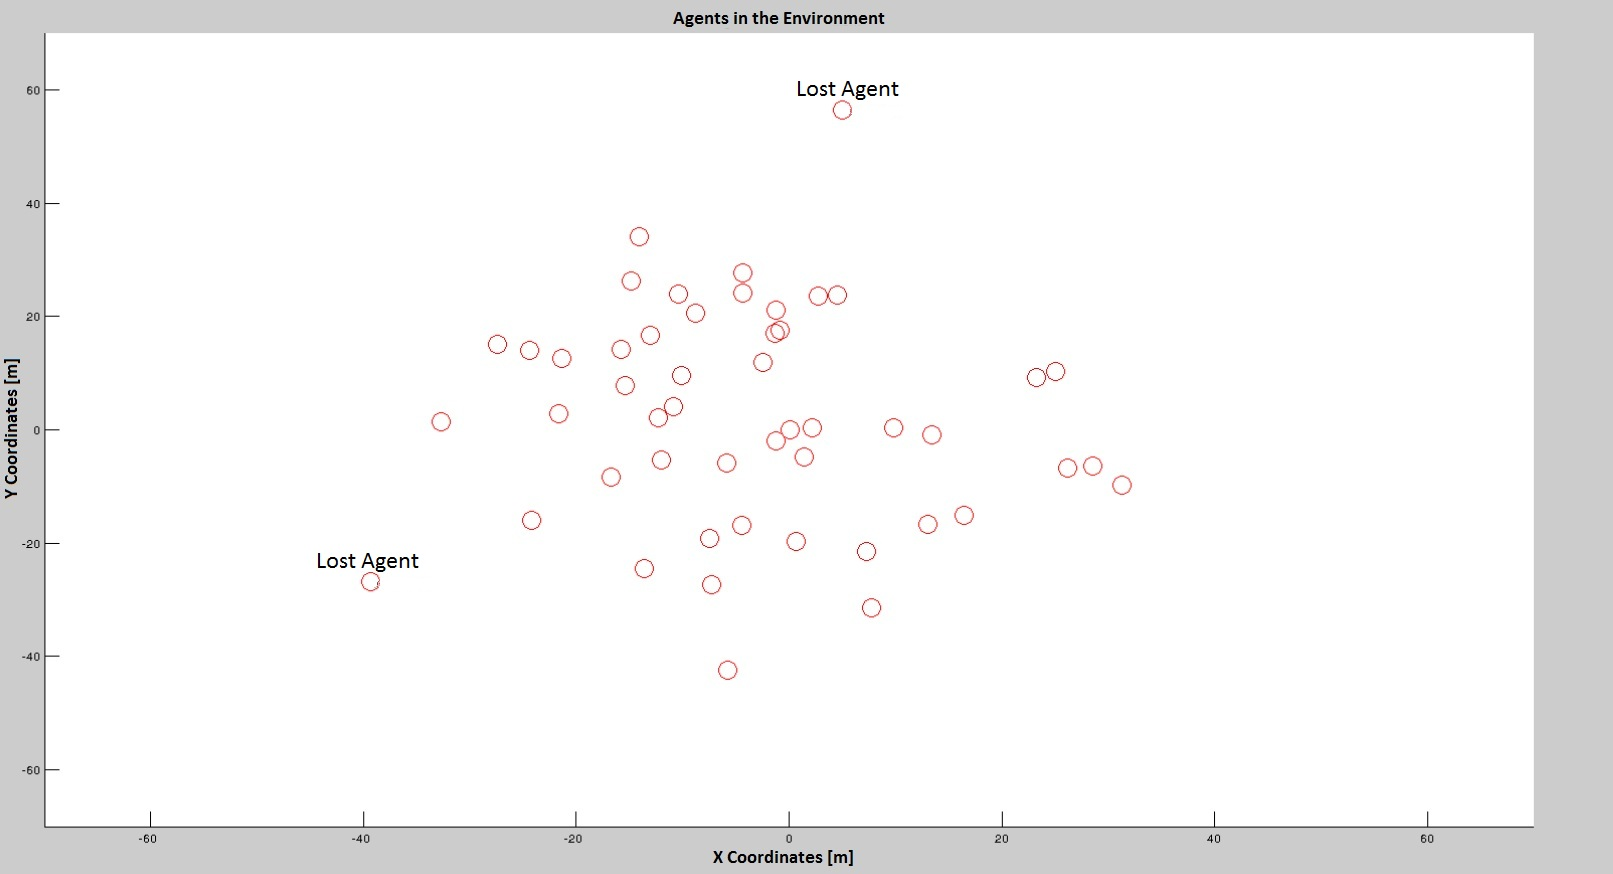
\includegraphics[scale = 0.25]{Lost-2-2}}
\end{figure} 

\begin{figure}[H]
\captionsetup{format=hang,justification=centerfirst}
\caption{Agents will be in 'Come Home' Mode After 3 Localization Period} \label{come_home_ref}
\centerline{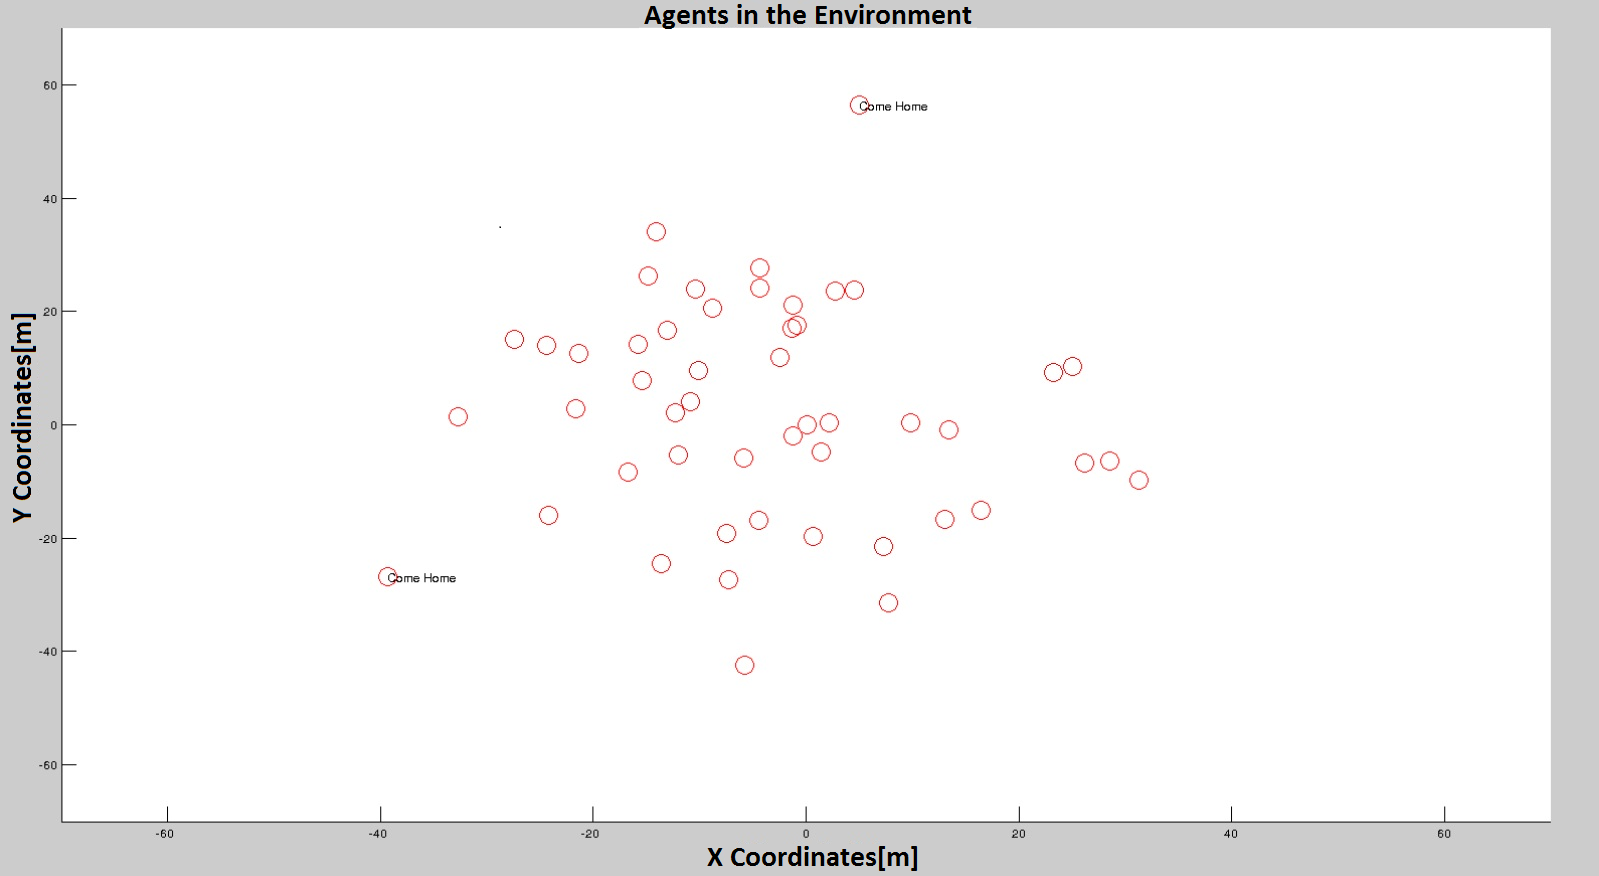
\includegraphics[scale = 0.25]{Lost-2-3}}
\end{figure} 		

		
\section{FORMATION CONTROL SYSTEM}
In this section, three different methods of which the details are presented in Section \ref{formation_control_ref} are evaluated according to their settling times, mesh qualities and total displacements. 

\subsection{Mesh Qualities} 
Mesh quality is a measure of how the agents homogeneously distributed while covering the desired formation shape. Basically, two different types of quality measurements defined in Section \ref{mesh_quality_ref} are used to evaluate the performance of the formation control methods, topological mesh irregularity $\epsilon_t$ and geometrical mesh irregularity $\epsilon_g$ . Monte Carlo simulations with 1000 iterations are handled for the same formation shapes with different initial conditions of the agents in the environment. Sample outputs for three different types of formation control algorithms are illustrated in the following figures. In these figures, red circles are representing the coverage circles of three different type of agents. Mesh irregularities are calculated by constructing the Voronoi diagrams with nodes located at the centers of these coverage circles.
  
\begin{figure}[H]
\caption{Shape 1 with Artificial Forces Methods:$\epsilon_t = 2.1$ and $\epsilon_g = 0.32$}
\centerline{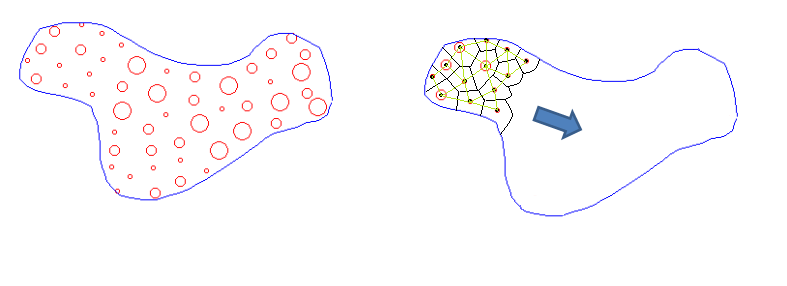
\includegraphics[scale = 0.70]{Artificial_Forces_Mesh_1}}
\end{figure} 		
		
\begin{figure}[H]
\caption{Shape 2 with Artificial Forces Methods:$\epsilon_t = 2.6$ and $\epsilon_g = 0.4$}
\centerline{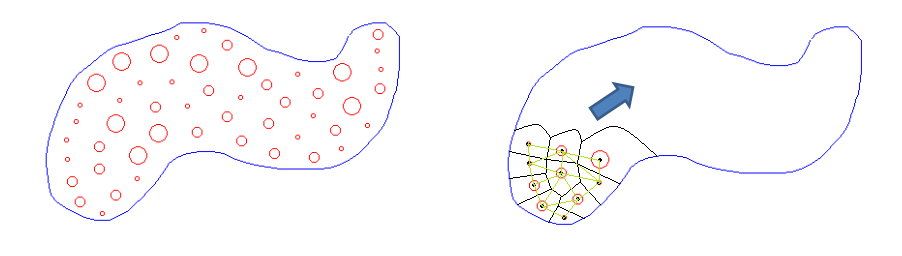
\includegraphics[scale = 0.65]{Artificial_Forces_Mesh_2}}
\end{figure} 		
		
\begin{figure}[H]
\caption{Shape 1 with Bubble Packing Method:$\epsilon_t = 2.1$ and $\epsilon_g = 0.24$}
\centerline{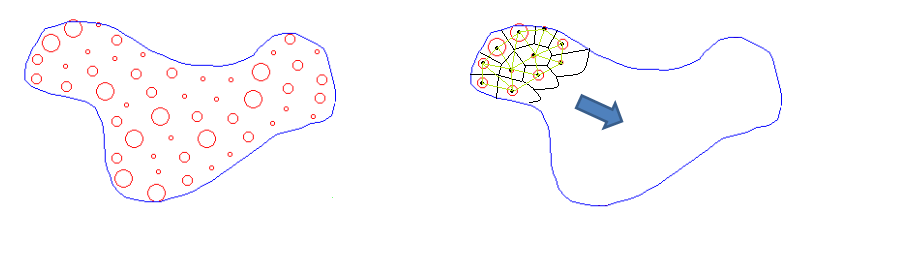
\includegraphics[scale = 0.70]{Bubble_Packing_Mesh_1}}
\end{figure} 	
				
\begin{figure}[H]
\caption{Shape 2 with Bubble Packing Method:$\epsilon_t = 2.3$ and $\epsilon_g = 0.28$}
\centerline{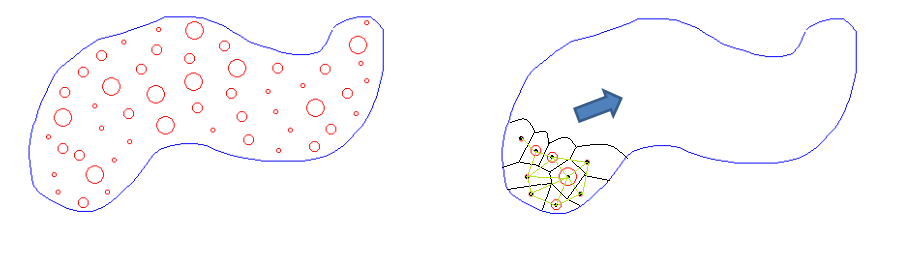
\includegraphics[scale = 0.65]{Bubble_Packing_Mesh_2}}
\end{figure} 			
						
\begin{figure}[H]
\caption{Shape 1 with Randomized Fractals Method:$\epsilon_t = 2.6$ and $\epsilon_g = 0.63$}
\centerline{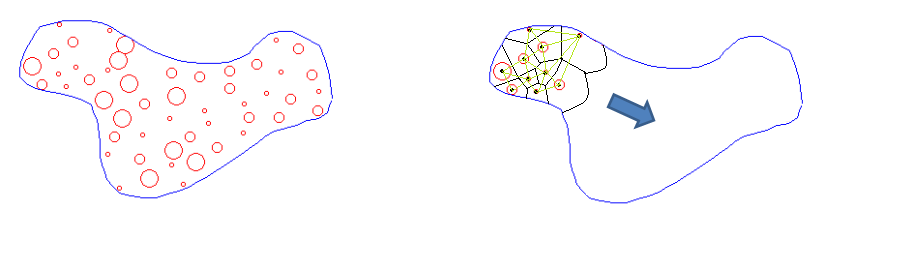
\includegraphics[scale = 0.70]{Randomized_Fractals_Mesh_1}}
\end{figure} 	

\begin{figure}[H]
\caption{Shape 2 with Randomized Fractal Method:$\epsilon_t = 3.1$ and $\epsilon_g = 0.61$}
\centerline{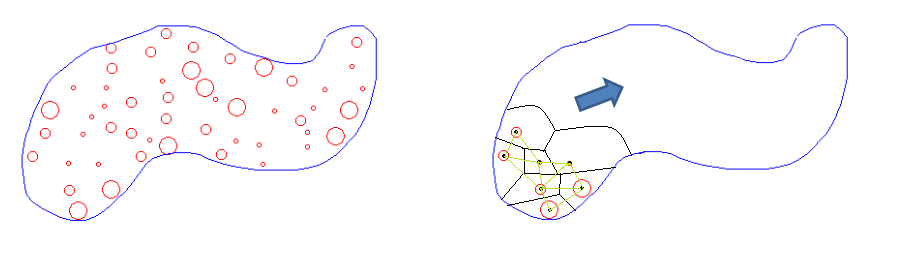
\includegraphics[scale = 0.65]{Randomized_Fractals_Mesh_2}}
\end{figure} 	

It can be concluded that Randomized Fractals method has the worst mesh performance. It is because of the randomized assignment of goal states into the formation shape in this methodology. Bubble Packing and Artificial Forces methods give similar results since they have an analogy in their approaches of implementing inter member/bubble forces which makes the agents/bubbles distributed in the formation shape more homogeneously. Artificial force method applies this intermember forces directly to the agents in formation control while Bubble Packing method use this force on artificial bubbles to partition the shape into goal states. Monte Carlo simulations with 1000 iterations for both formation shapes with different initial conditions are handled and the results are illustrated in Figure \ref{topologic_ref_1}; \ref{geometric_ref_1}; \ref{topologic_ref_2}; \ref{geometric_ref_2} . Randomized Fractals method have greater mean values for both topological and geometrical mesh irregularities as expected.  Bubble Packing and Artificial Forces methods have similar performances on mesh quality.
		
\begin{figure}[H]
\caption{Formation Shape 1 Topological Mesh Irregularities} \label{topologic_ref_1}
\centerline{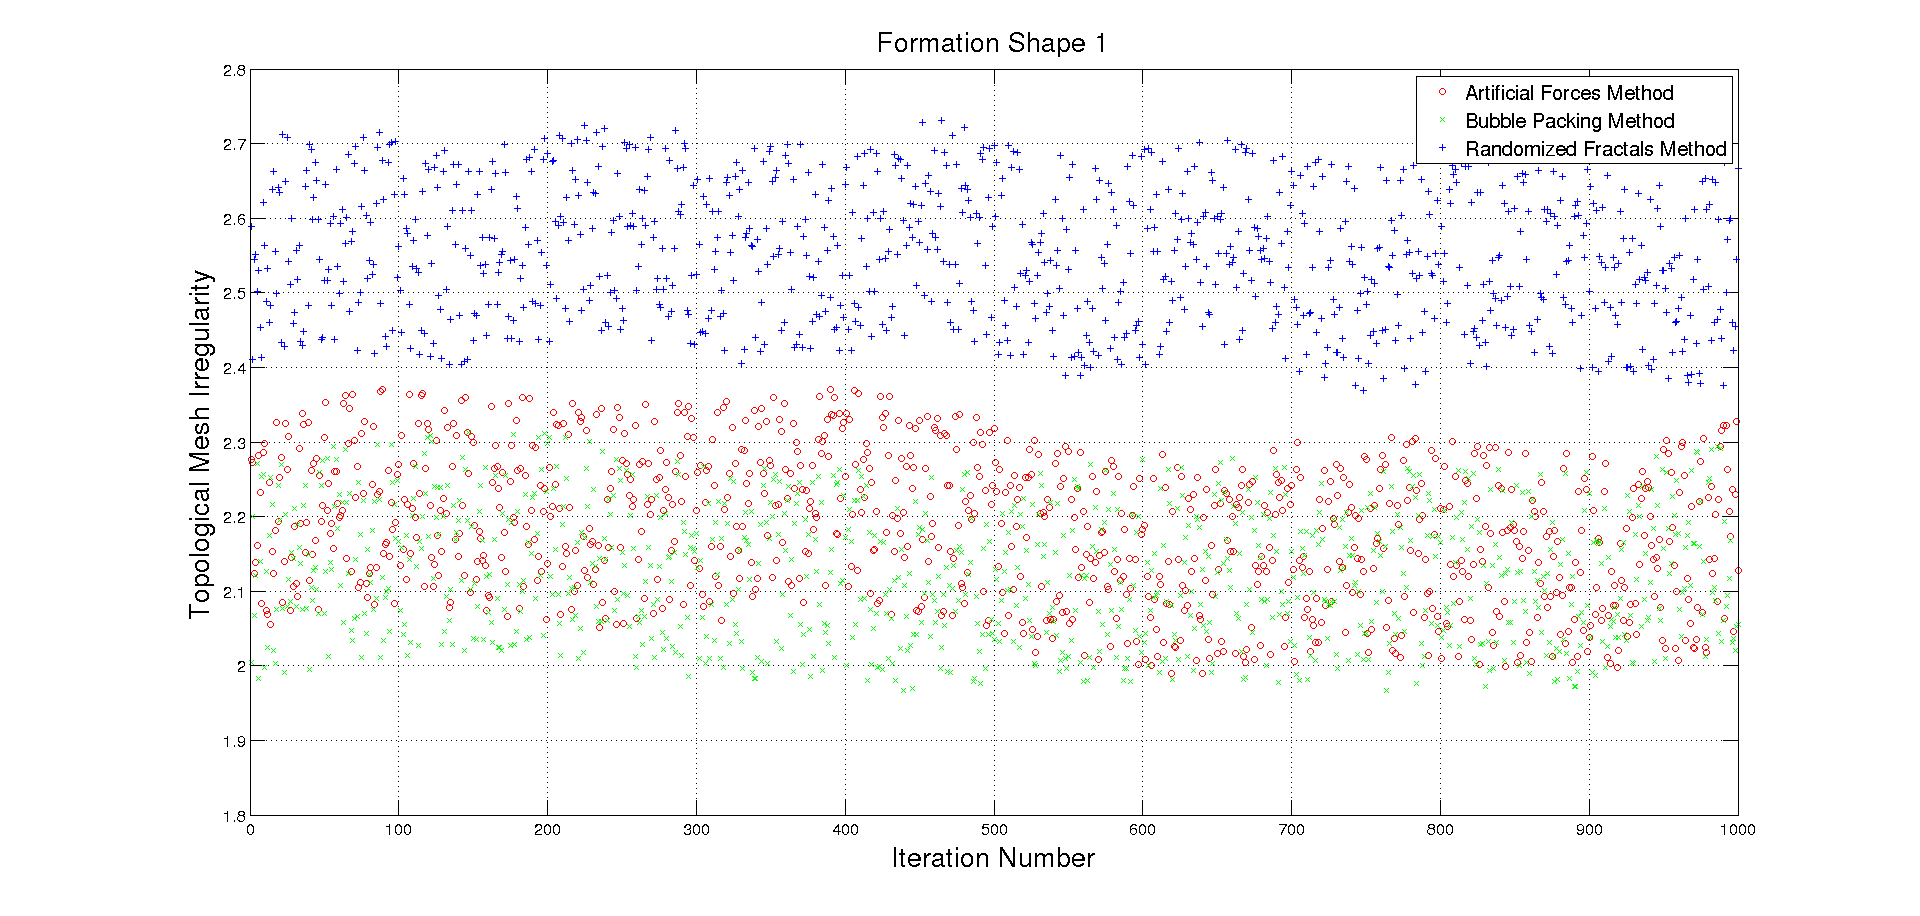
\includegraphics[scale = 0.35]{Topological_Irr_1}}
\end{figure} 	
		
\begin{figure}[H]
\caption{Formation Shape 1 Geometrical Mesh Irregularities} \label{geometric_ref_1}
\centerline{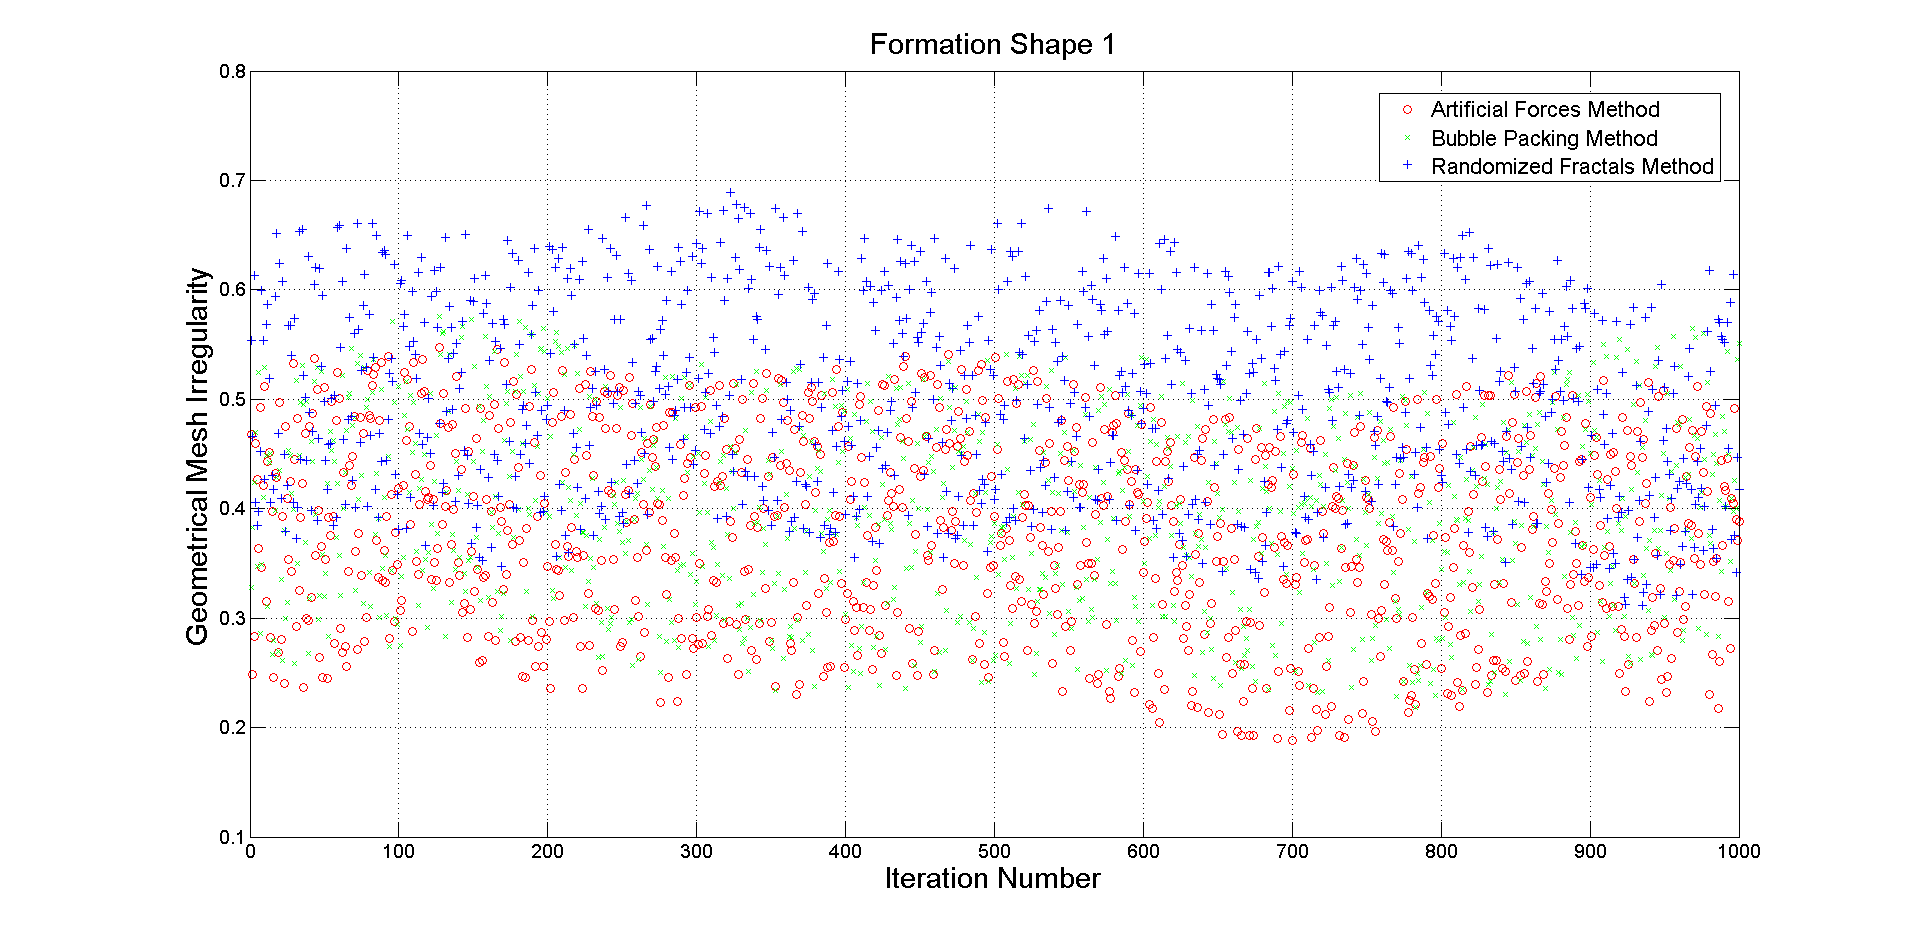
\includegraphics[scale = 0.35]{Geometrical_Irr_1}}
\end{figure} 	

\begin{figure}[H]
\caption{Formation Shape 2 Topological Mesh Irregularities} \label{topologic_ref_2}
\centerline{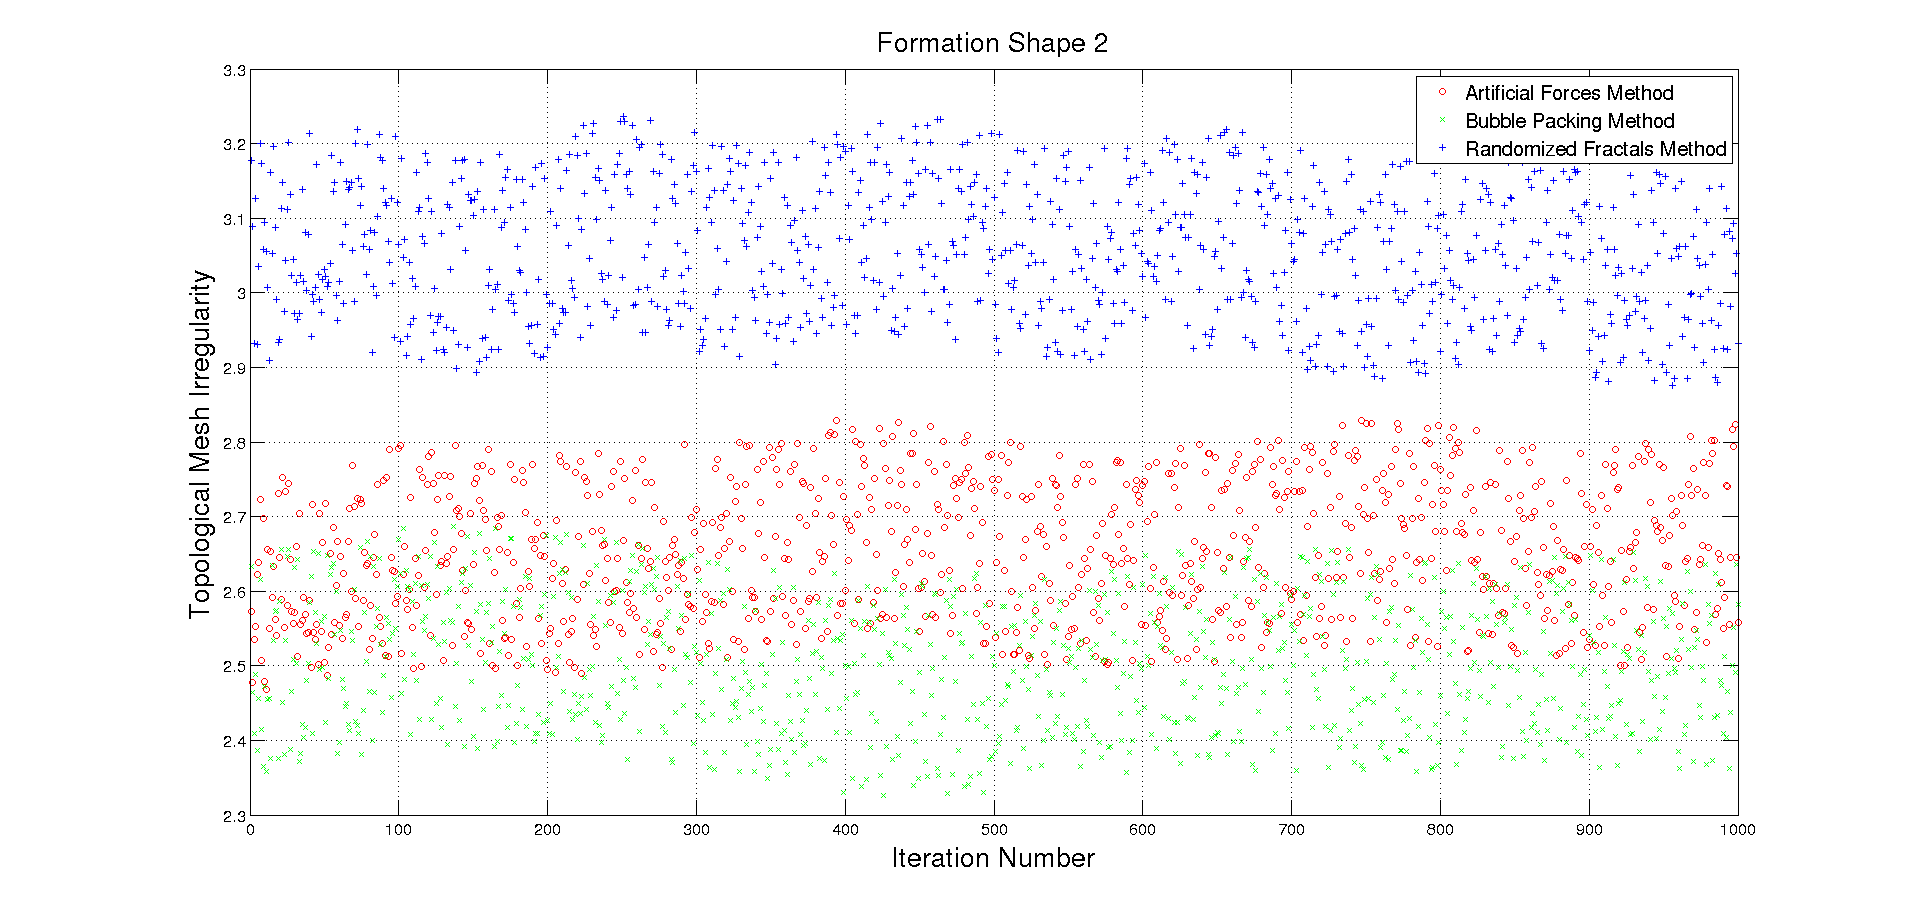
\includegraphics[scale = 0.35]{Topological_Irr_2}}
\end{figure} 	
				
\begin{figure}[H]
\caption{Formation Shape 2 Geometrical Mesh Irregularities} \label{geometric_ref_2}
\centerline{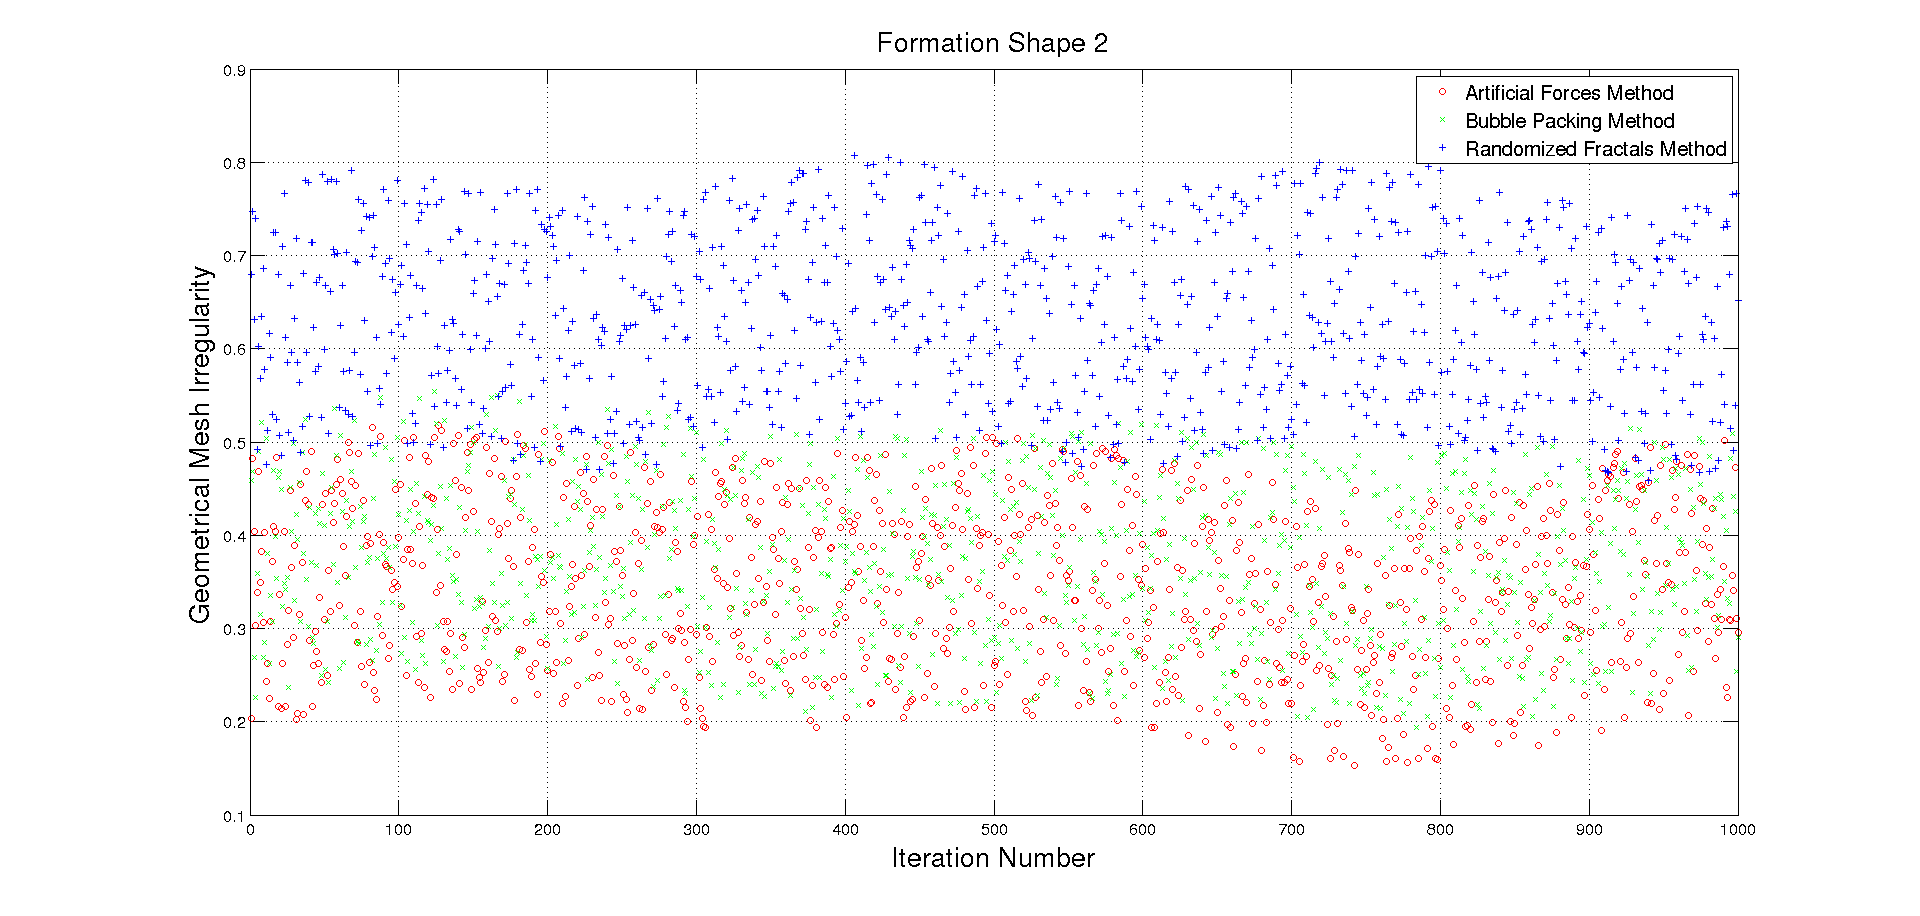
\includegraphics[scale = 0.35]{Geometrical_Irr_2}}
\end{figure} 	
		
\subsection{Total Displacement of the Agents}  \label{total_dist_ref}
		
In this project, we aim to minimize the overall displacement of the agents in the swarm while getting the desired formation shape. Here the main approach is to reduce down the expected energy consumption of the swarm by decreasing the required displacements. To compare the total displacement of the swarm while getting the desired shape for three different methods, we have done Monte Carlo simulations with 1000 iterations. These simulations are handled for the same formation shapes with different initial conditions of the agents in the environment. Trajectories of the agents are recorded from the initial positions to the goal states for three different types of formation control systems. Sample outputs for three different types of formation control algorithms are illustrated in the following figures.
		
\subsubsection{Shape 1}\hspace{0pt} \\
		
\begin{figure}[H]
\caption{Formation Shape 1 in MATLAB environment}
\centerline{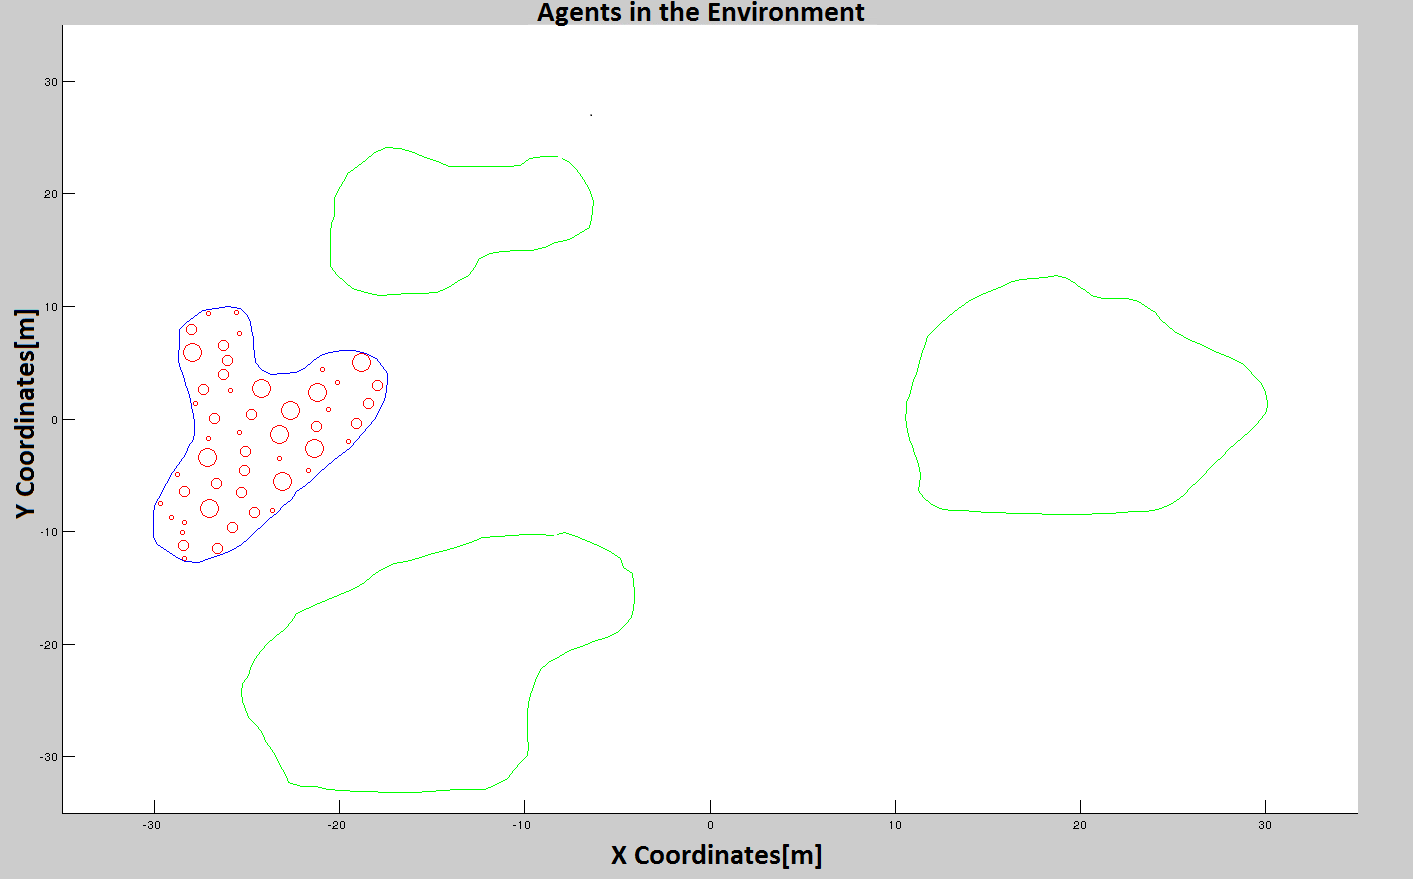
\includegraphics[scale = 0.32]{Trajectories_Formation_Shape_1_2}}
\end{figure} 	
			
\begin{figure}[H]
\caption{Formation Shape 1 in Gazebo environment}
\centerline{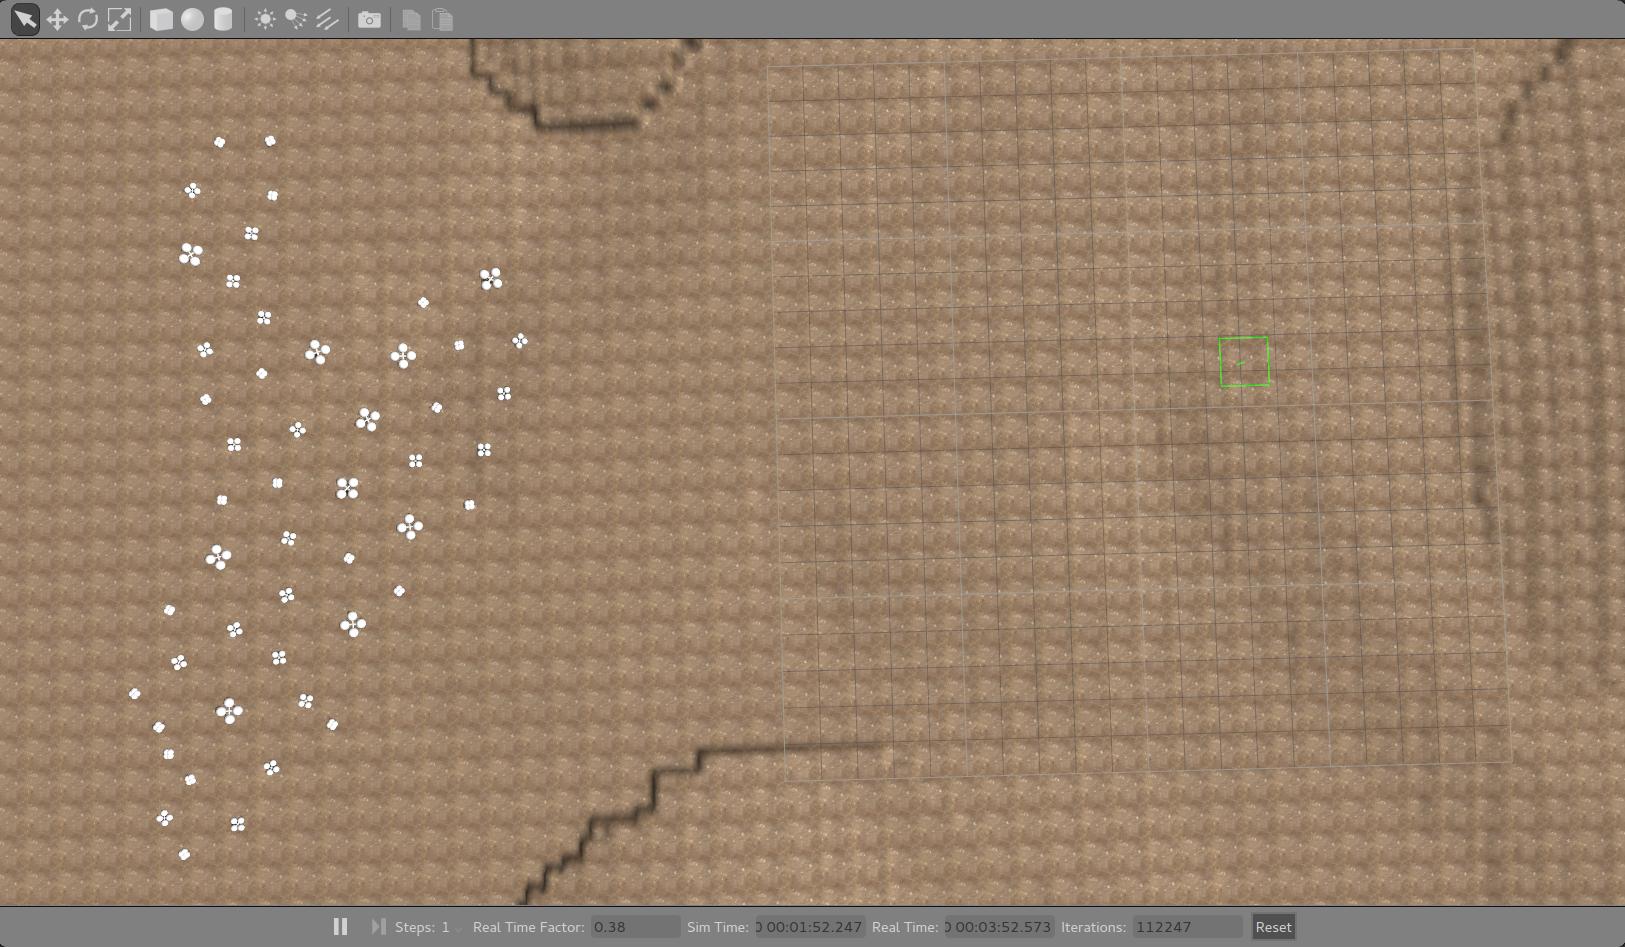
\includegraphics[scale = 0.32]{Trajectories_Formation_Shape_1_1}}
\end{figure} 	
		
\begin{figure}[H]
\caption{Artificial Forces Method Trajectories for Shape 1}
\centerline{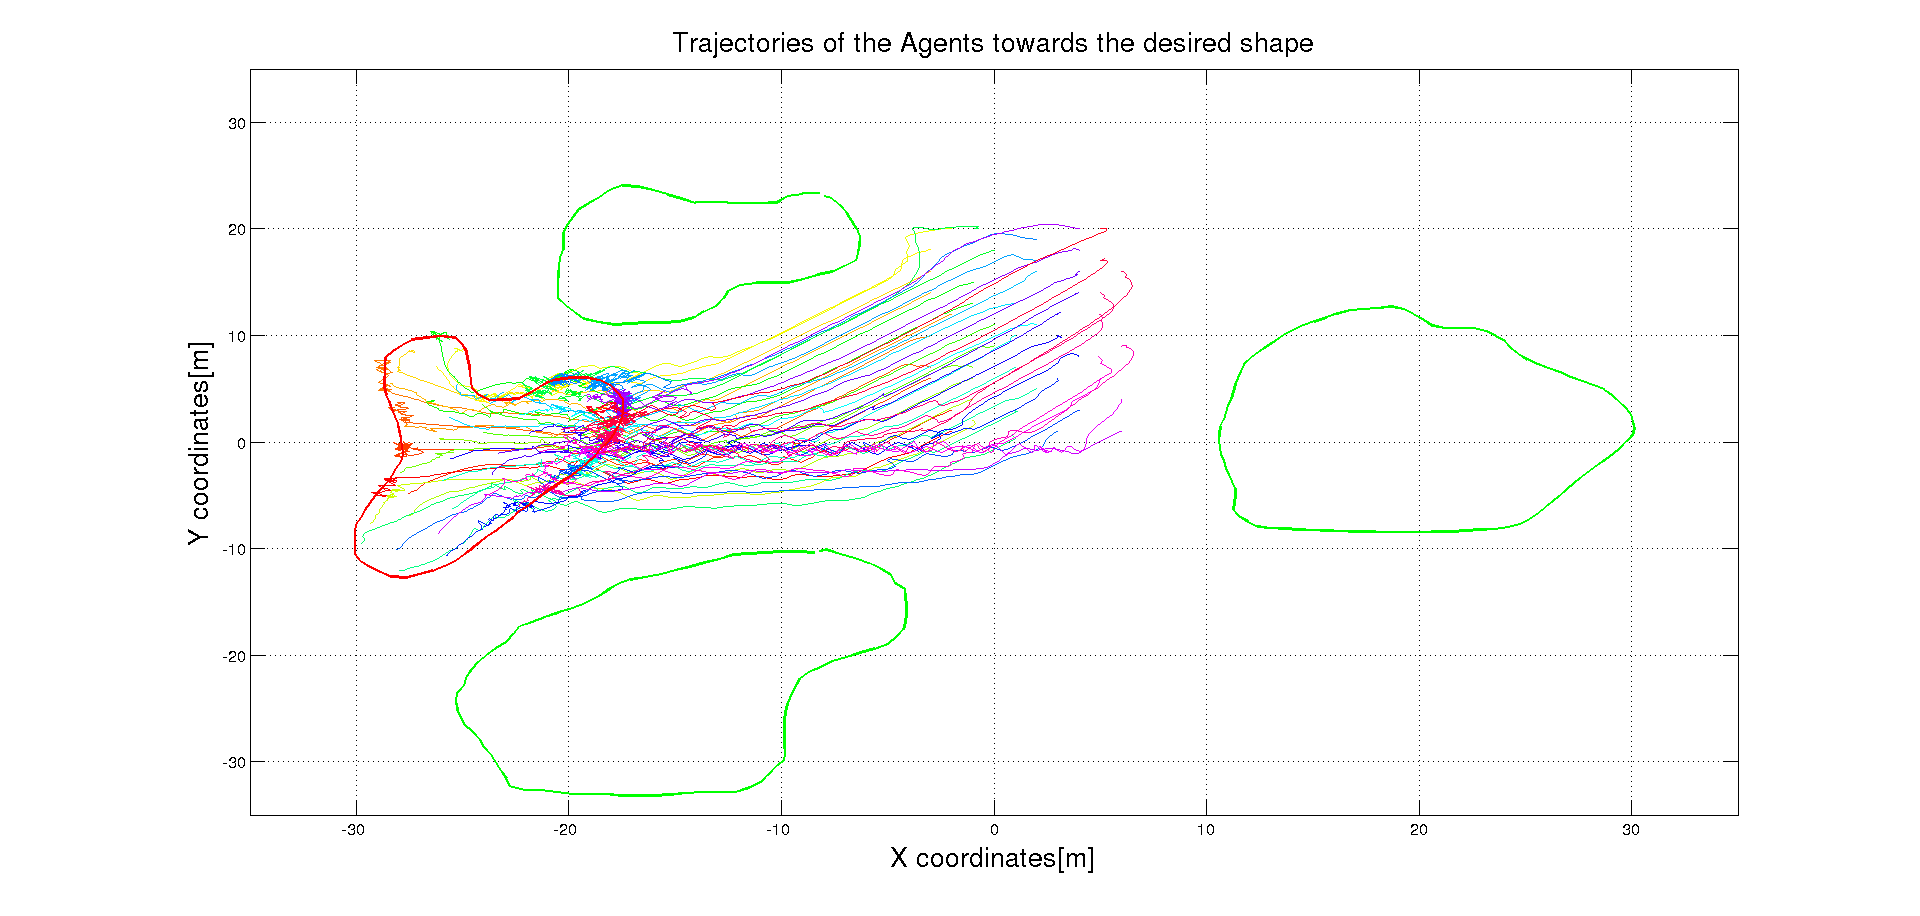
\includegraphics[scale = 0.32]{Aritificial_Trajecories_1}}
\end{figure} 	

\begin{figure}[H]
\caption{Bubble Packing Method Trajectories for Shape 1}
\centerline{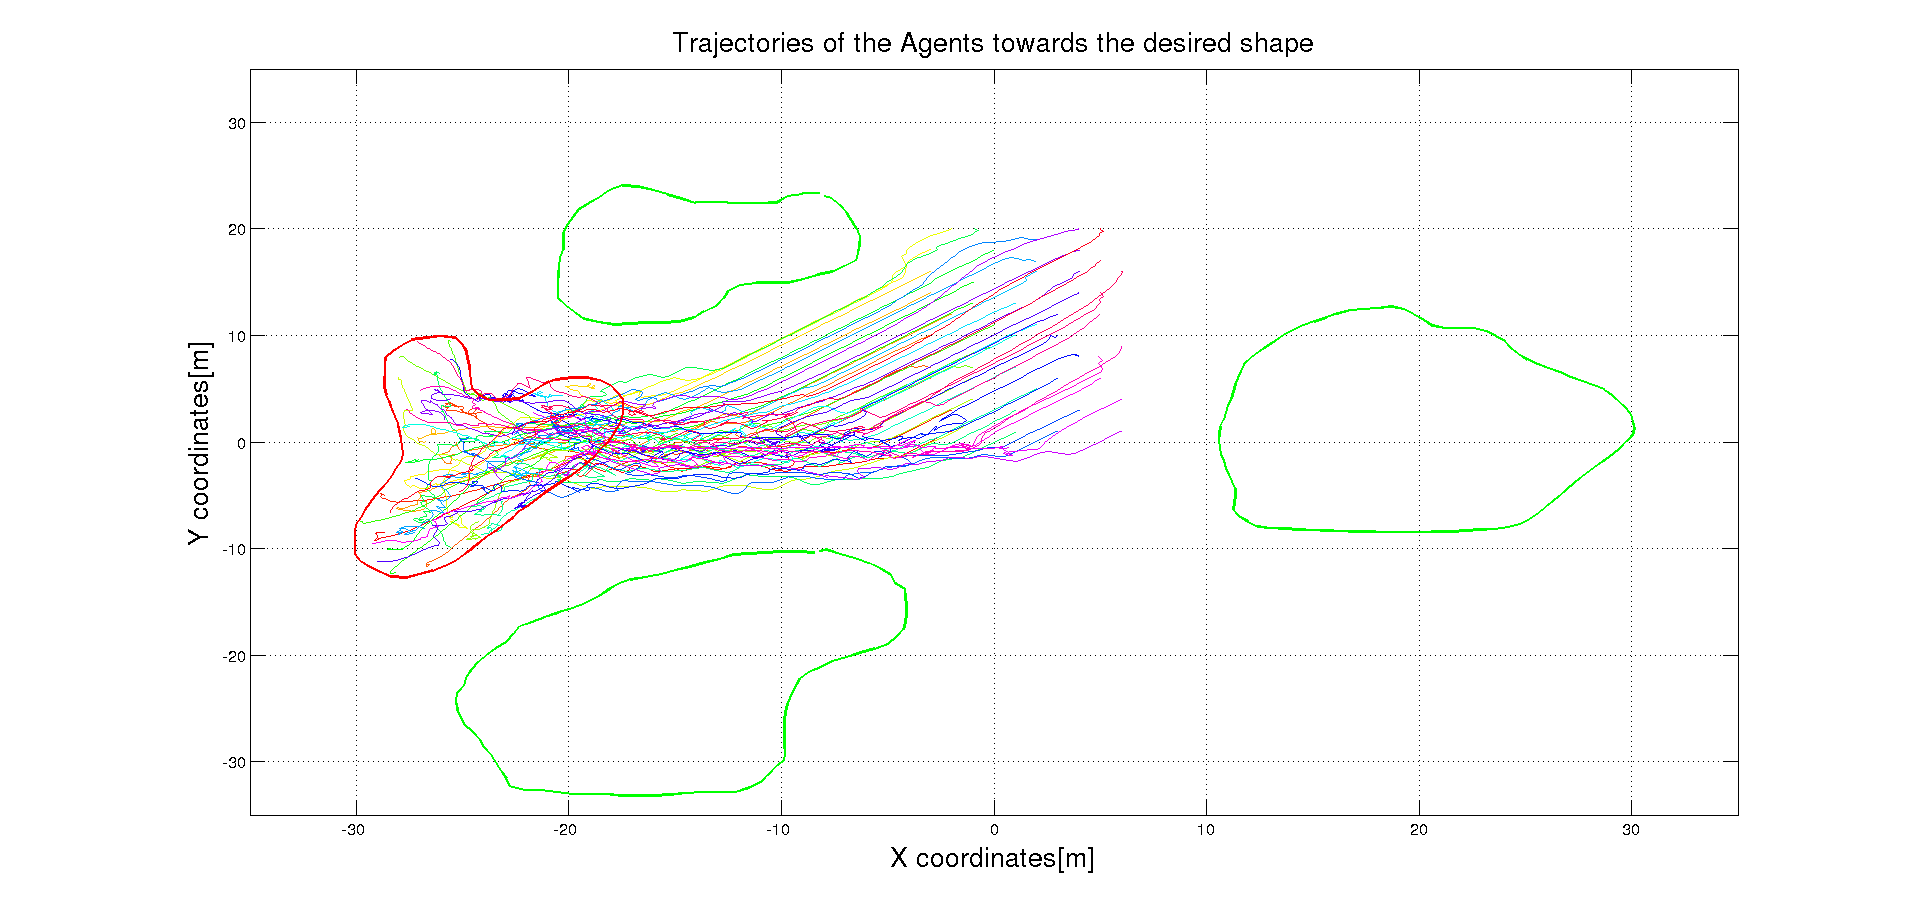
\includegraphics[scale = 0.32]{Bubble_Trajectories_1}}
\end{figure} 	
		
\begin{figure}[H]
\caption{Randomized Fractals Method Trajectories for Shape 1}
\centerline{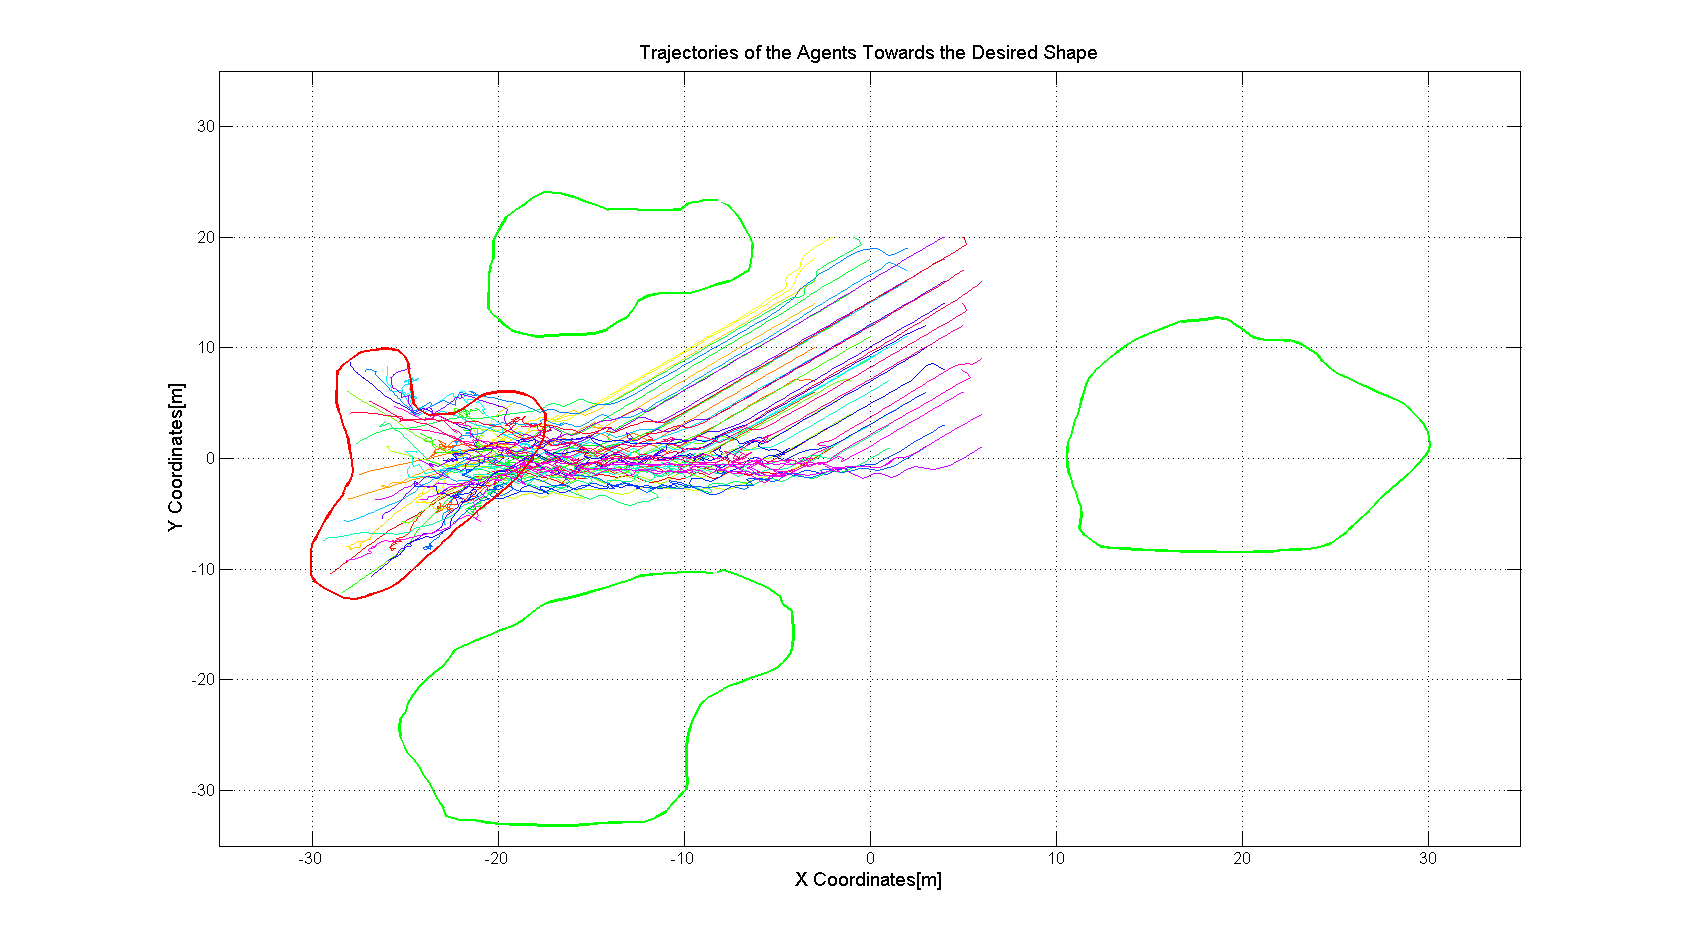
\includegraphics[scale = 0.32]{Randomized_Trajectories_1}}
\end{figure} 	
			
It can be seen that the trajectories of the agents are more chaotic and complex in the Artificial Forces method according to the other two solutions. Main cause for this situation, the agents are under the effect of a total force which is instantly changing both amplitude and direction with the local interactions with the environment in Artificial Forces method. The only force component which provides the distribution of the agents in the formation shape homogeneously is the intermember forces which is dynamically changing so much with the local instant neighbors of the agents in the environment. On the other hand, Bubble Packing and Randomized Fractal methods implement an algorithm in which every agent is directed to a goal state in which the total displacements in the environment is minimized. This approach prevents the chaotic appearance of the trajectories and minimizes the displacements of the agents. Because agent are trying to reach their goal states directly within these two methods. 

To compare the total displacements, we have done Monte Carlo simulations with 1000 iterations and the results are presented in Figure \ref{total_disp_1}. According to this figure, Artificial Forces method has a higher mean value of total travelled distance while achieving the same formation shape with same initial conditions. Performances of Bubble Packing and Randomized Fractals method seem similar, because the only difference between these two methods is their shape partitioning approaches. The assignment procedure of the agents to these goal states by minimizing the total displacement is implemented identically. 
		
\begin{figure}[H]
\caption{Total Travelled Distances for Shape 1} \label{total_disp_1}
\centerline{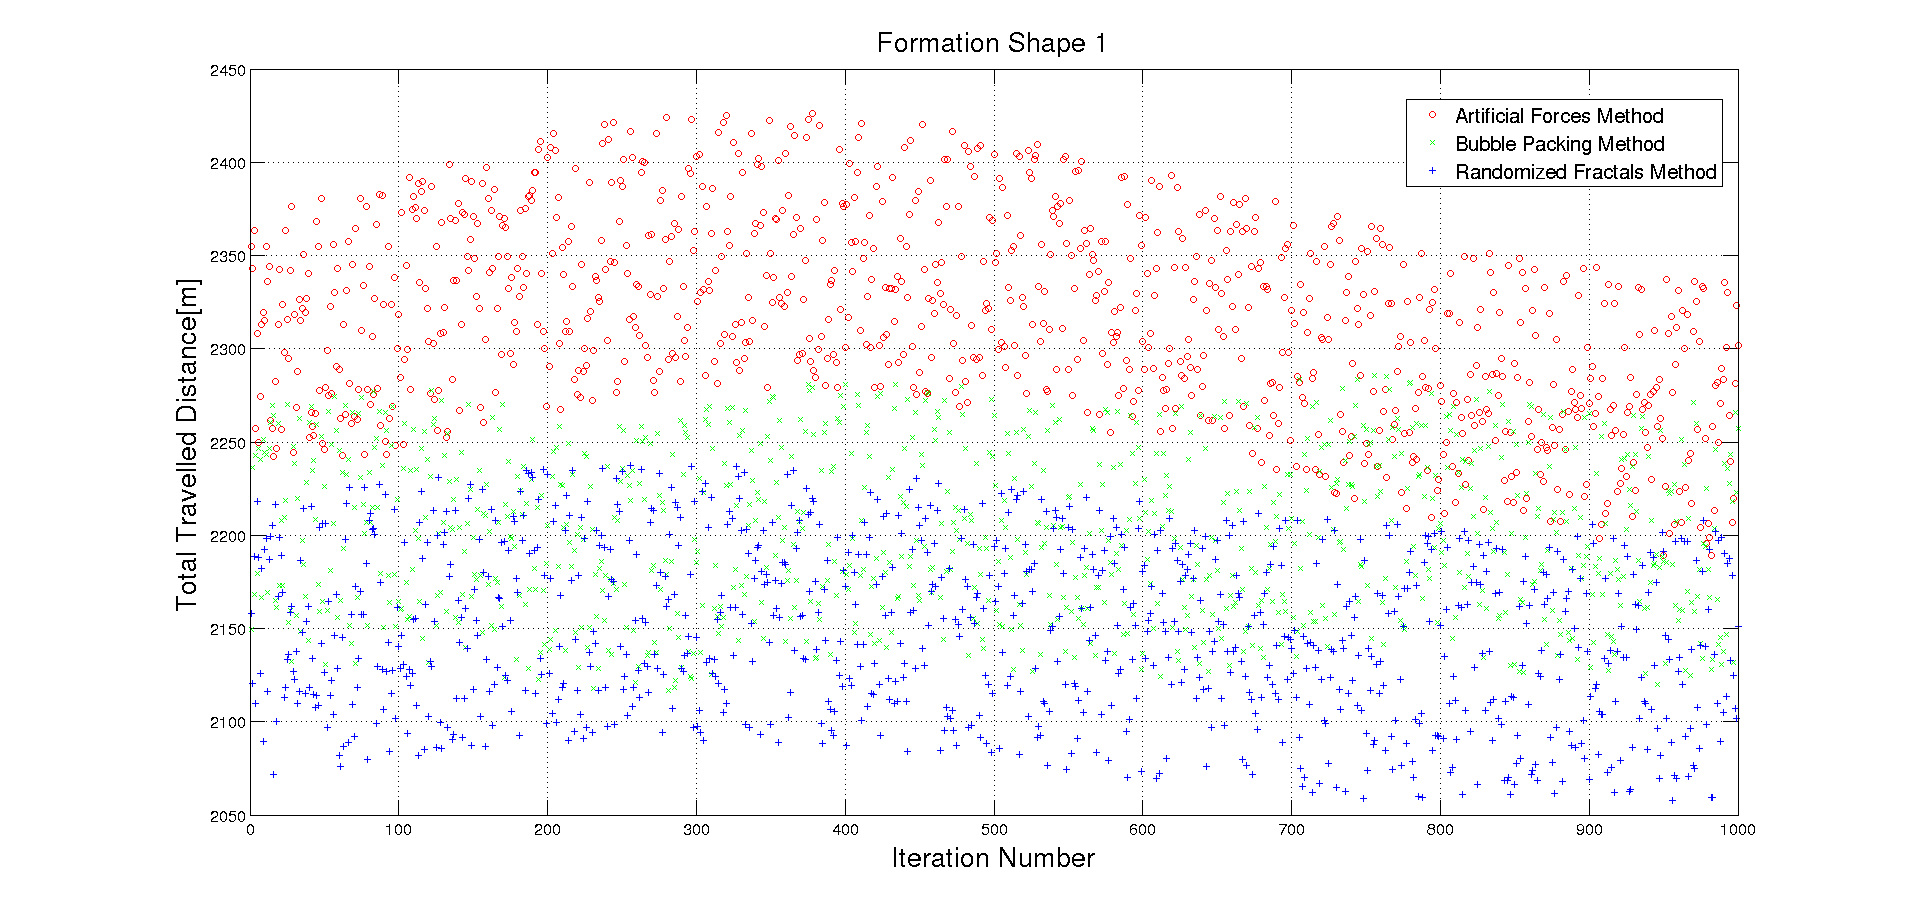
\includegraphics[scale = 0.32]{Total_Energy_Shape_1}}
\end{figure} 	
				
\subsubsection{Shape 2}\hspace{0pt} \\
Second formation shape gives similar results with three different formation control methods, because of the reasons discussed for the Formation Shape 1. Artifical Forces method has the worst performance on total travelled distance metric. 

\begin{figure}[H]
\caption{Formation Shape 2 in MATLAB environment}
\centerline{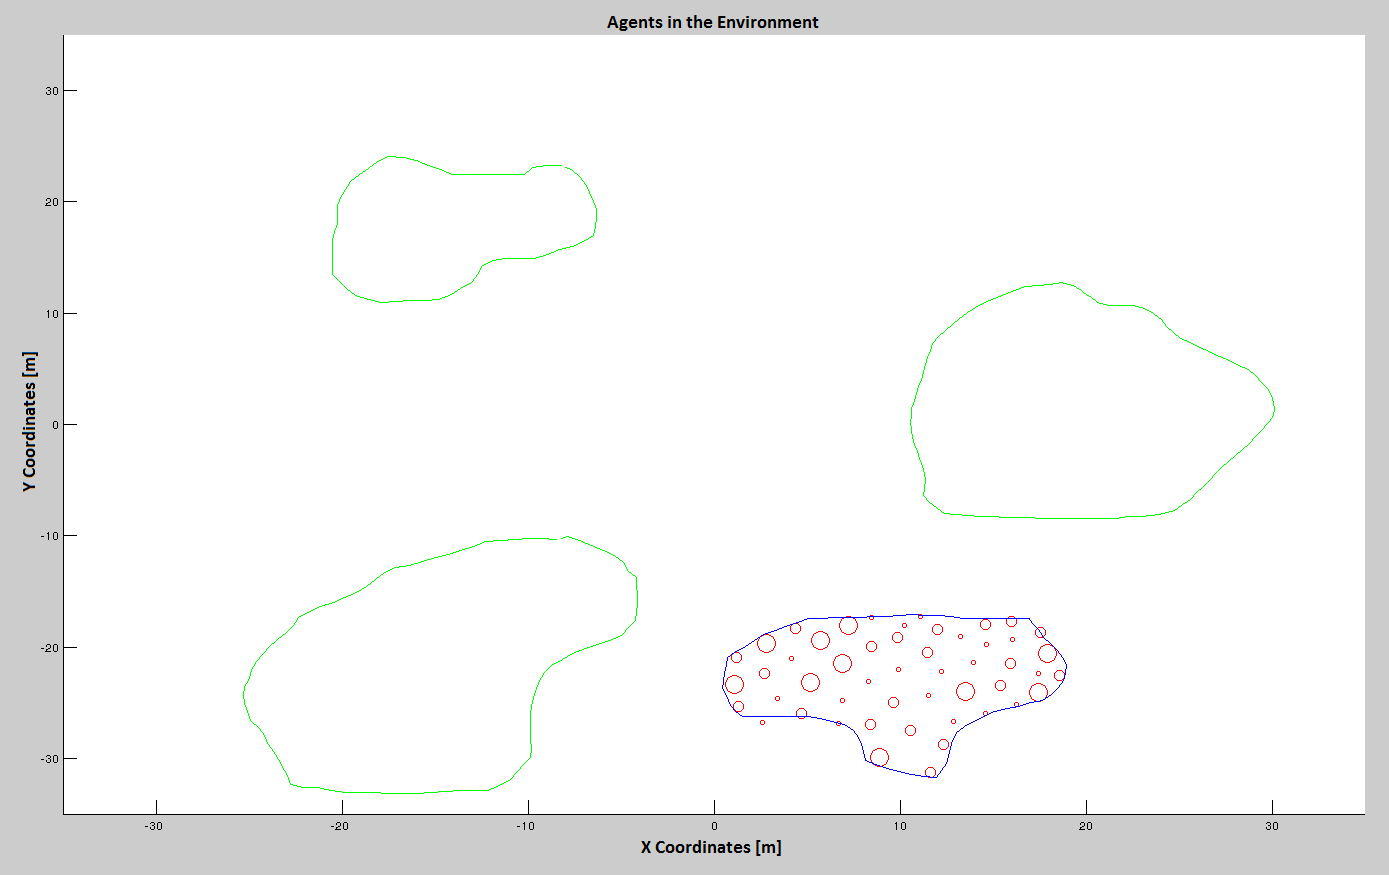
\includegraphics[scale = 0.32]{Trajectories_Formation_Shape_2_2}}
\end{figure} 	
		   
\begin{figure}[H]
\caption{Formation Shape 2 in Gazebo environment}
\centerline{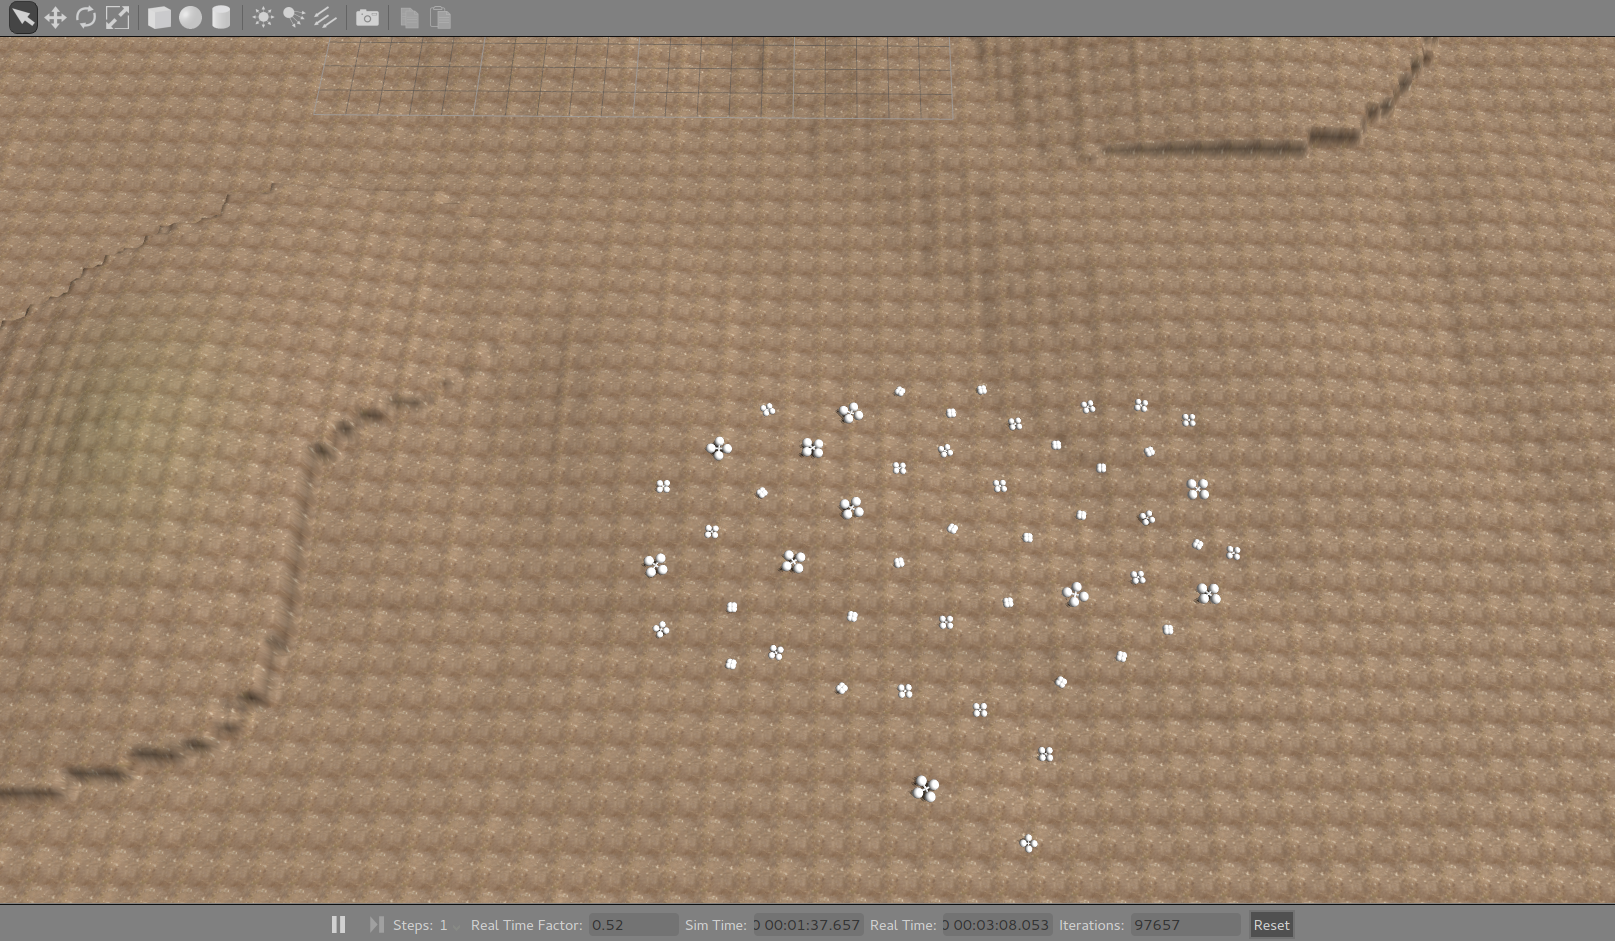
\includegraphics[scale = 0.32]{Trajectories_Formation_Shape_2_1}}
\end{figure} 	
		   
\begin{figure}[H]
\caption{Artificial Forces Method Trajectories for Shape 2}
\centerline{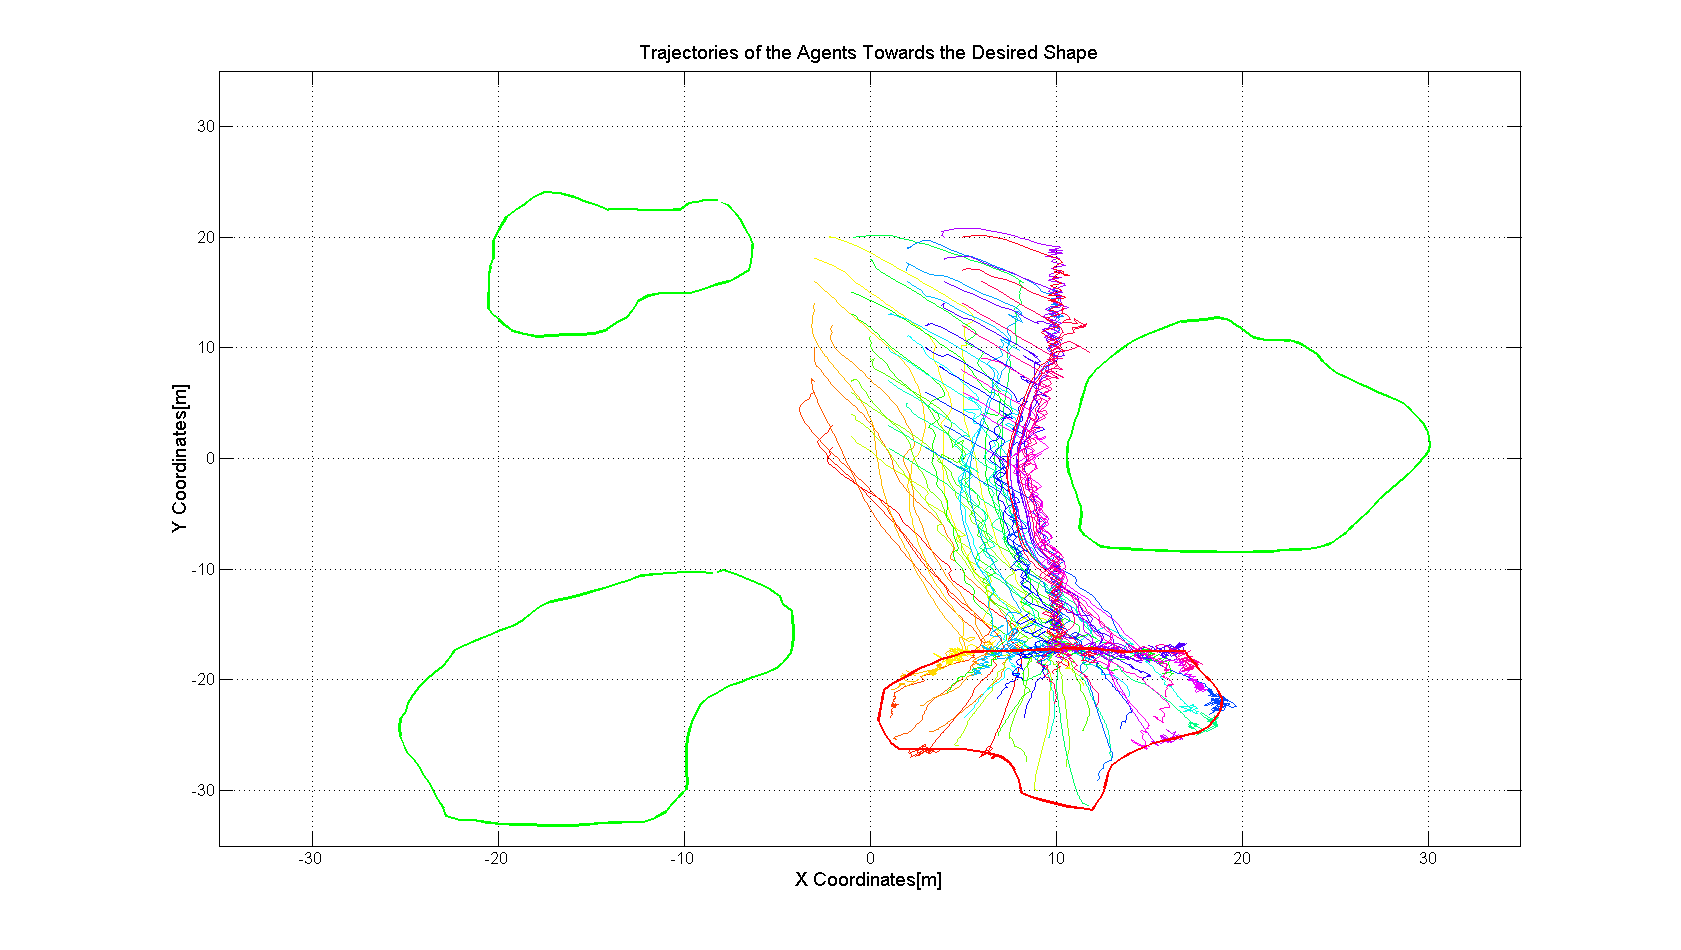
\includegraphics[scale = 0.32]{Artificial_Trajectories_2}}
\end{figure} 	
		   
\begin{figure}[H]
\caption{Bubble Packing Method Trajectories for Shape 2}
\centerline{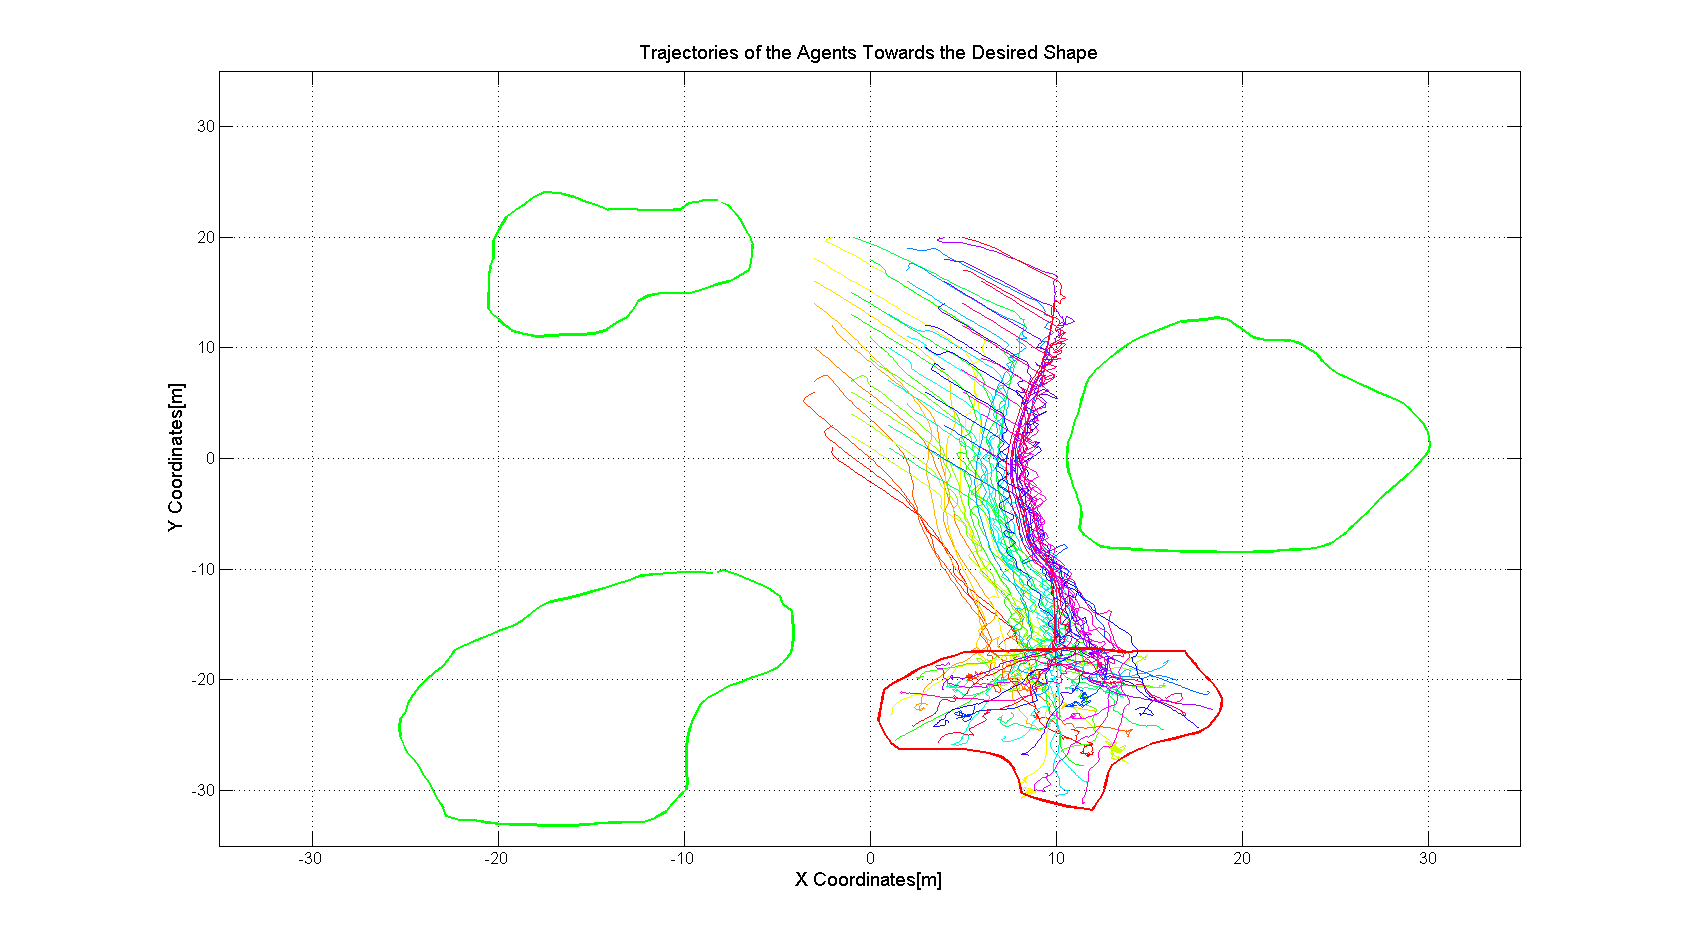
\includegraphics[scale = 0.32]{Bubble_Trajectories_2}}
\end{figure} 	
		   
\begin{figure}[H]
\caption{Randomized Fractals Method Trajectories for Shape 2}
\centerline{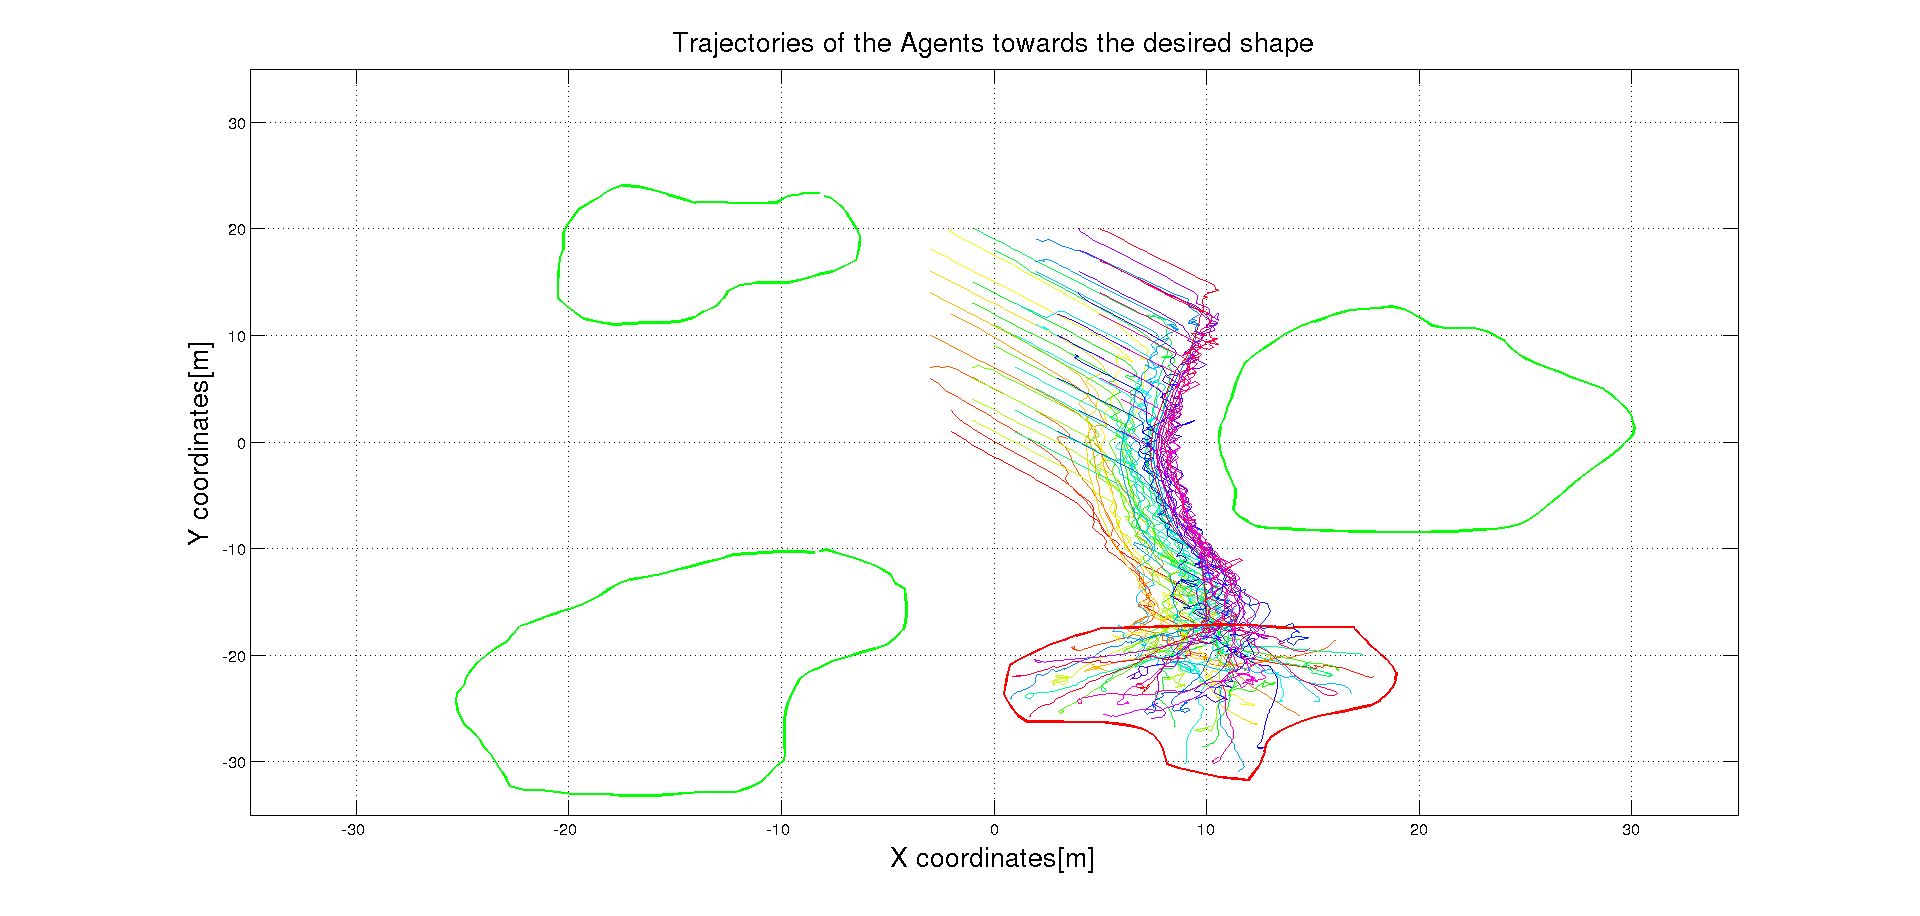
\includegraphics[scale = 0.32]{Randomized_Trajectories_2}}
\end{figure} 	
		   
The results of the Monte Carlo simulations with 1000 iterations are illustrated in Figure \ref{total_dist_2} . In this figure, Artificial Forces method has a higher mean value on total travelled distance for the same formation shape with same initial conditions. 

\begin{figure}[H]
\caption{Total Travelled Distance for Shape 2} \label{total_dist_2}
\centerline{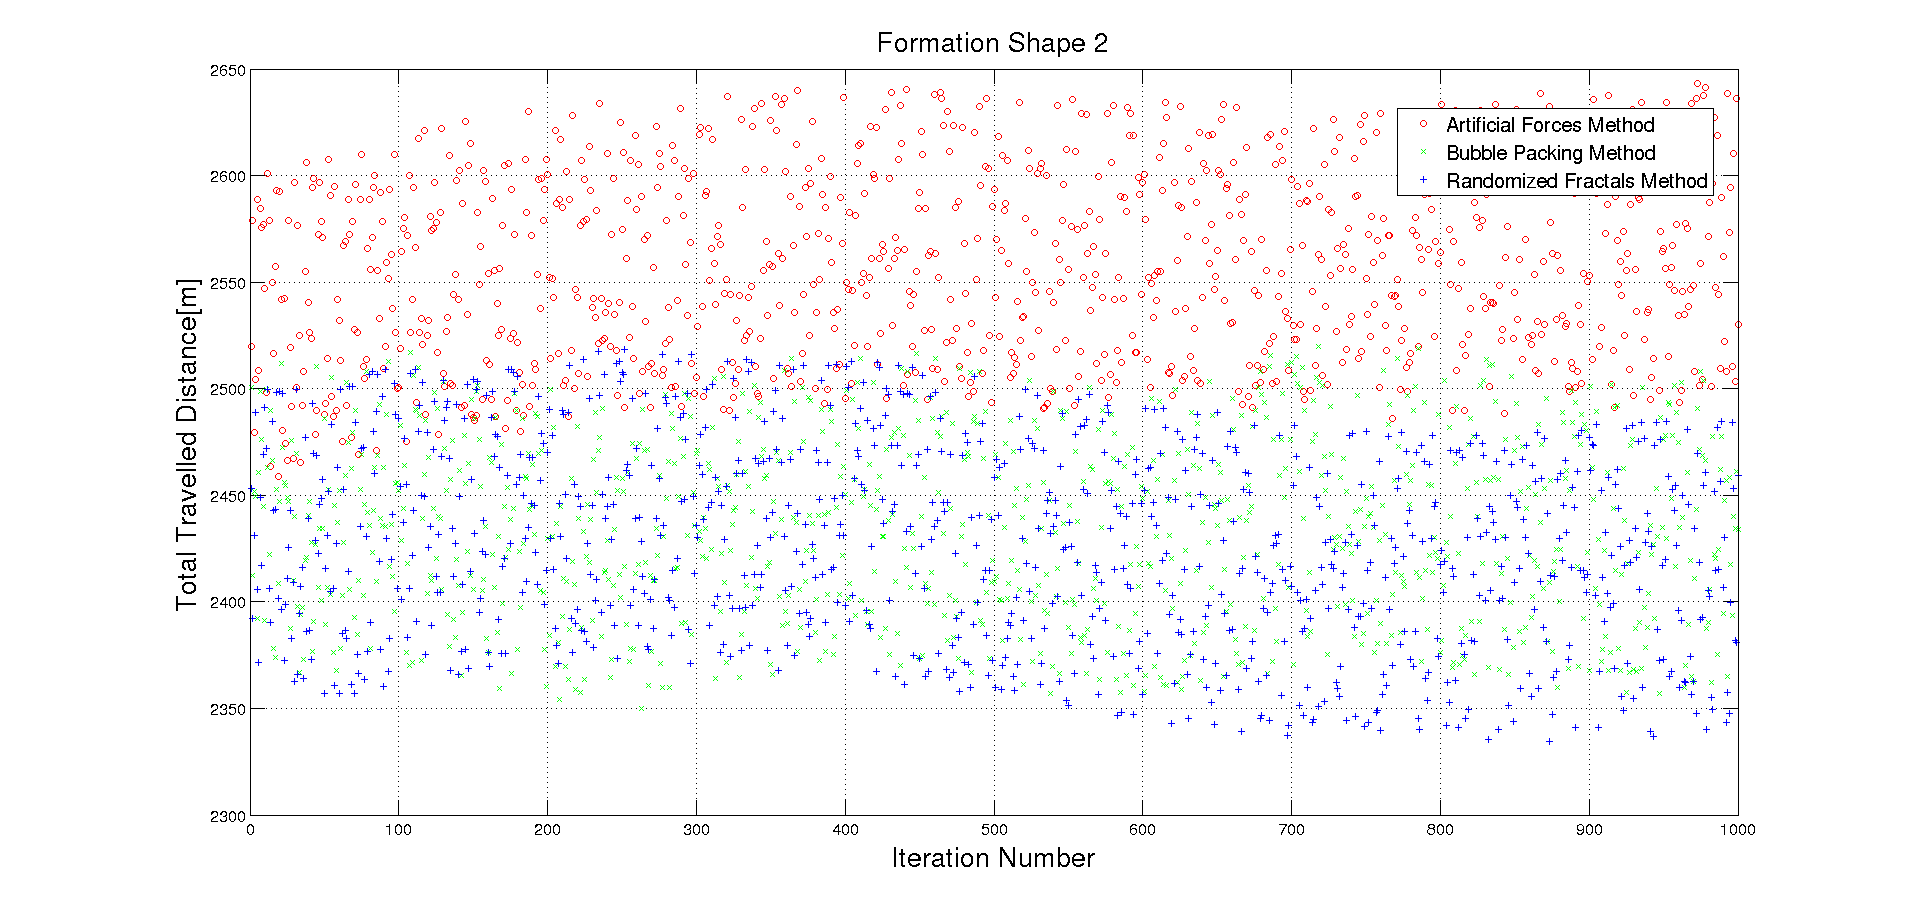
\includegraphics[scale = 0.32]{Total_Energy_Shape_2}} 
\end{figure} 	
		   
\subsection{Settling Time} \label{settling_ref}
Settling time is defined as delta time $"t_{final} - t_{start}"$ ,where $t_{start}$ is the initial time and $t_{final}$ is the time that the all of the agents are inside of the desired formation shape and the norm of the velocity vector for each agent $\norm{v_i}$ is
		
\begin{equation}
\norm{v_i(t)} < 0.01 \hspace{0.1cm} [m/sec] \hspace{0.3cm}\forall\hspace{0.05cm} t>t_{final}
\end{equation}
		
To compare the settling time performances of three different methods, we have measured the settling times for the simulations held in Section \ref{total_dist_ref}. Artificial Forces method has the worst performance because agents are expected to need more time to reach the steady state under the effect of different artificial force components. Since there are no predetermined goal states for the agents in the desired formation shape, the settling of the agents in random places under the equilibrium of the artificial force components takes more time than the other two formation control methods. The agents have reached the steady state at their goal states with the Bubble Packing and Randomized Fractals methods faster than the Artificial Forces Methods. The results are illustrated in Figure \ref{settling_1} and \ref{settling_2}. According to these figures, Artificial Forces method has a higher mean value on settling time higher than the other two methods.
		
\begin{figure}[H]
\caption{Total Settling Time for Shape 1} \label{settling_1}
\centerline{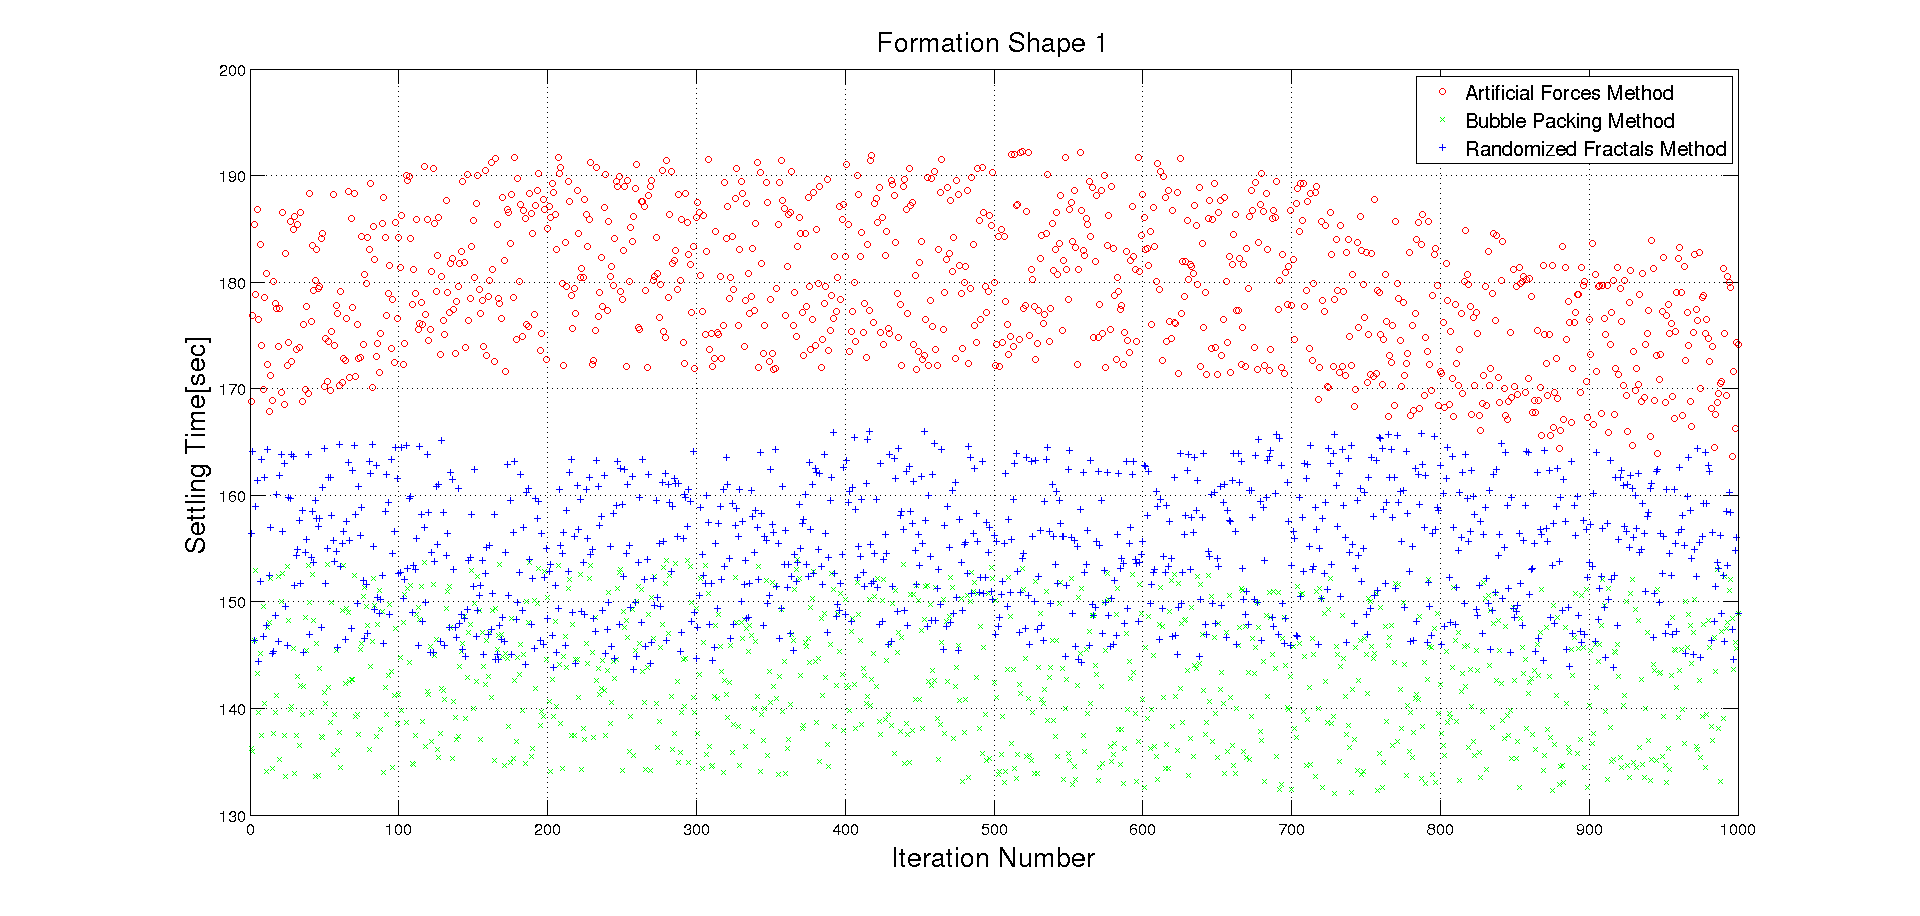
\includegraphics[scale = 0.32]{Total_Time_Shape_1}}
\end{figure} 
		
\begin{figure}[H]
\caption{Total Settling Time for Shape 2} \label{settling_2}
\centerline{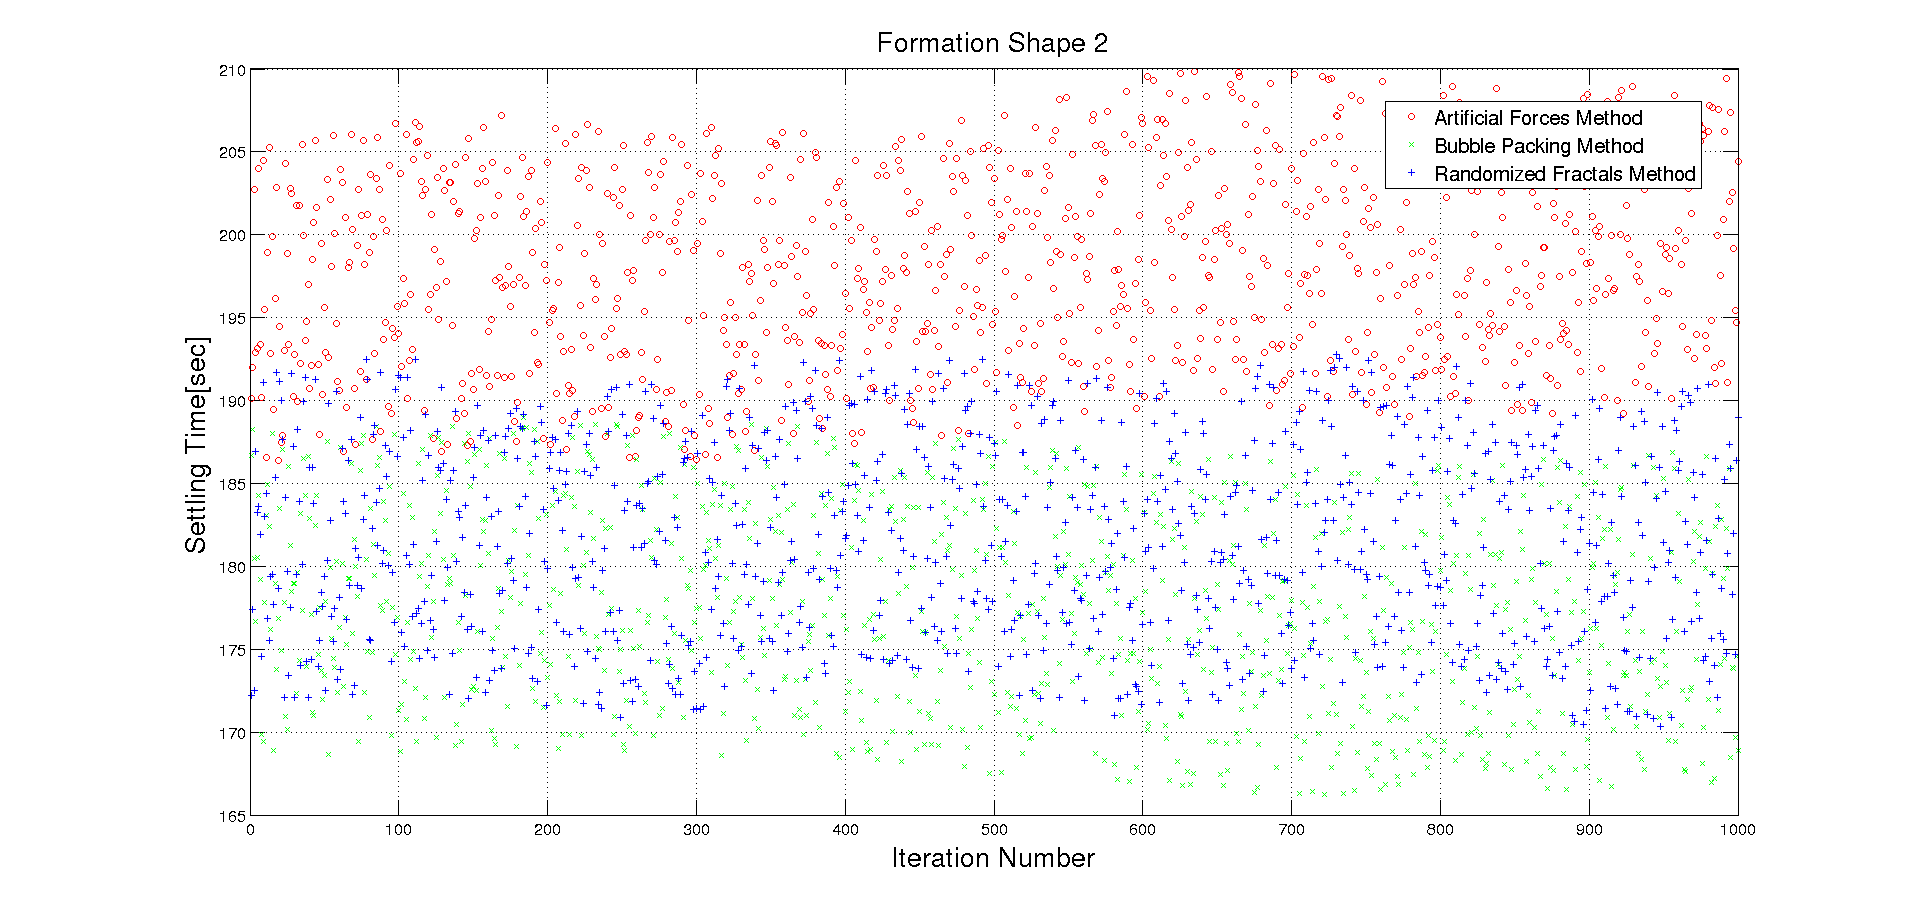
\includegraphics[scale = 0.32]{Total_Time_Shape_2}}
\end{figure} 

\subsection{Dynamically Changing Formations} \label{dynamical_ref}
In dynamic formation control, desired formation shape is changed dynamically in a smooth fashion. Agents have to adapt themselves to this changing formation shape and cover the shape in a continuous manner. Since the formation shape is expected to have smooth changes in local regions, it is aimed to adapt the agents which are positioned at these local regions rather than replacing all agents simultaneously. To minimize the total displacement of the swarm, the general approach is to make the agents which are close to the changing regions take action and replace themselves while other ones which are far away from that region keeps their positions. Randomized fractals method doesn't have a solution for this type of problem since its nature of randomly assignment of agents in a given formation shape. These assignments made by the randomized fractals method will not have continuous transitions on goal states between sequential formation shapes changing with execution period of the algorithm. On the other hand, it is possible to adapt the Bubble Packing algorithm to provide a solution for the dynamically changing formations. Since Bubble Packing algorithm determines goal states in a formation shape by applying interbubble forces, it is possible to keep this shape partitioning process running in background and dynamically adapt the goal states to the changing formation shape. The assignments to these goal states with Hungarian algorithm will adapt the swarm to the dynamically changing formation shape. Artificial forces method calculates control inputs for the individuals according to the current environment conditions and the formation shape. There is no need to update the algorithm for dynamically changing formation shapes, it already supports dynamically changing formations. 
		 
\begin{figure}[H]
\caption{Dynamic Formation Control with Bubble Packing Method} \label{multiple1_ref}
\centerline{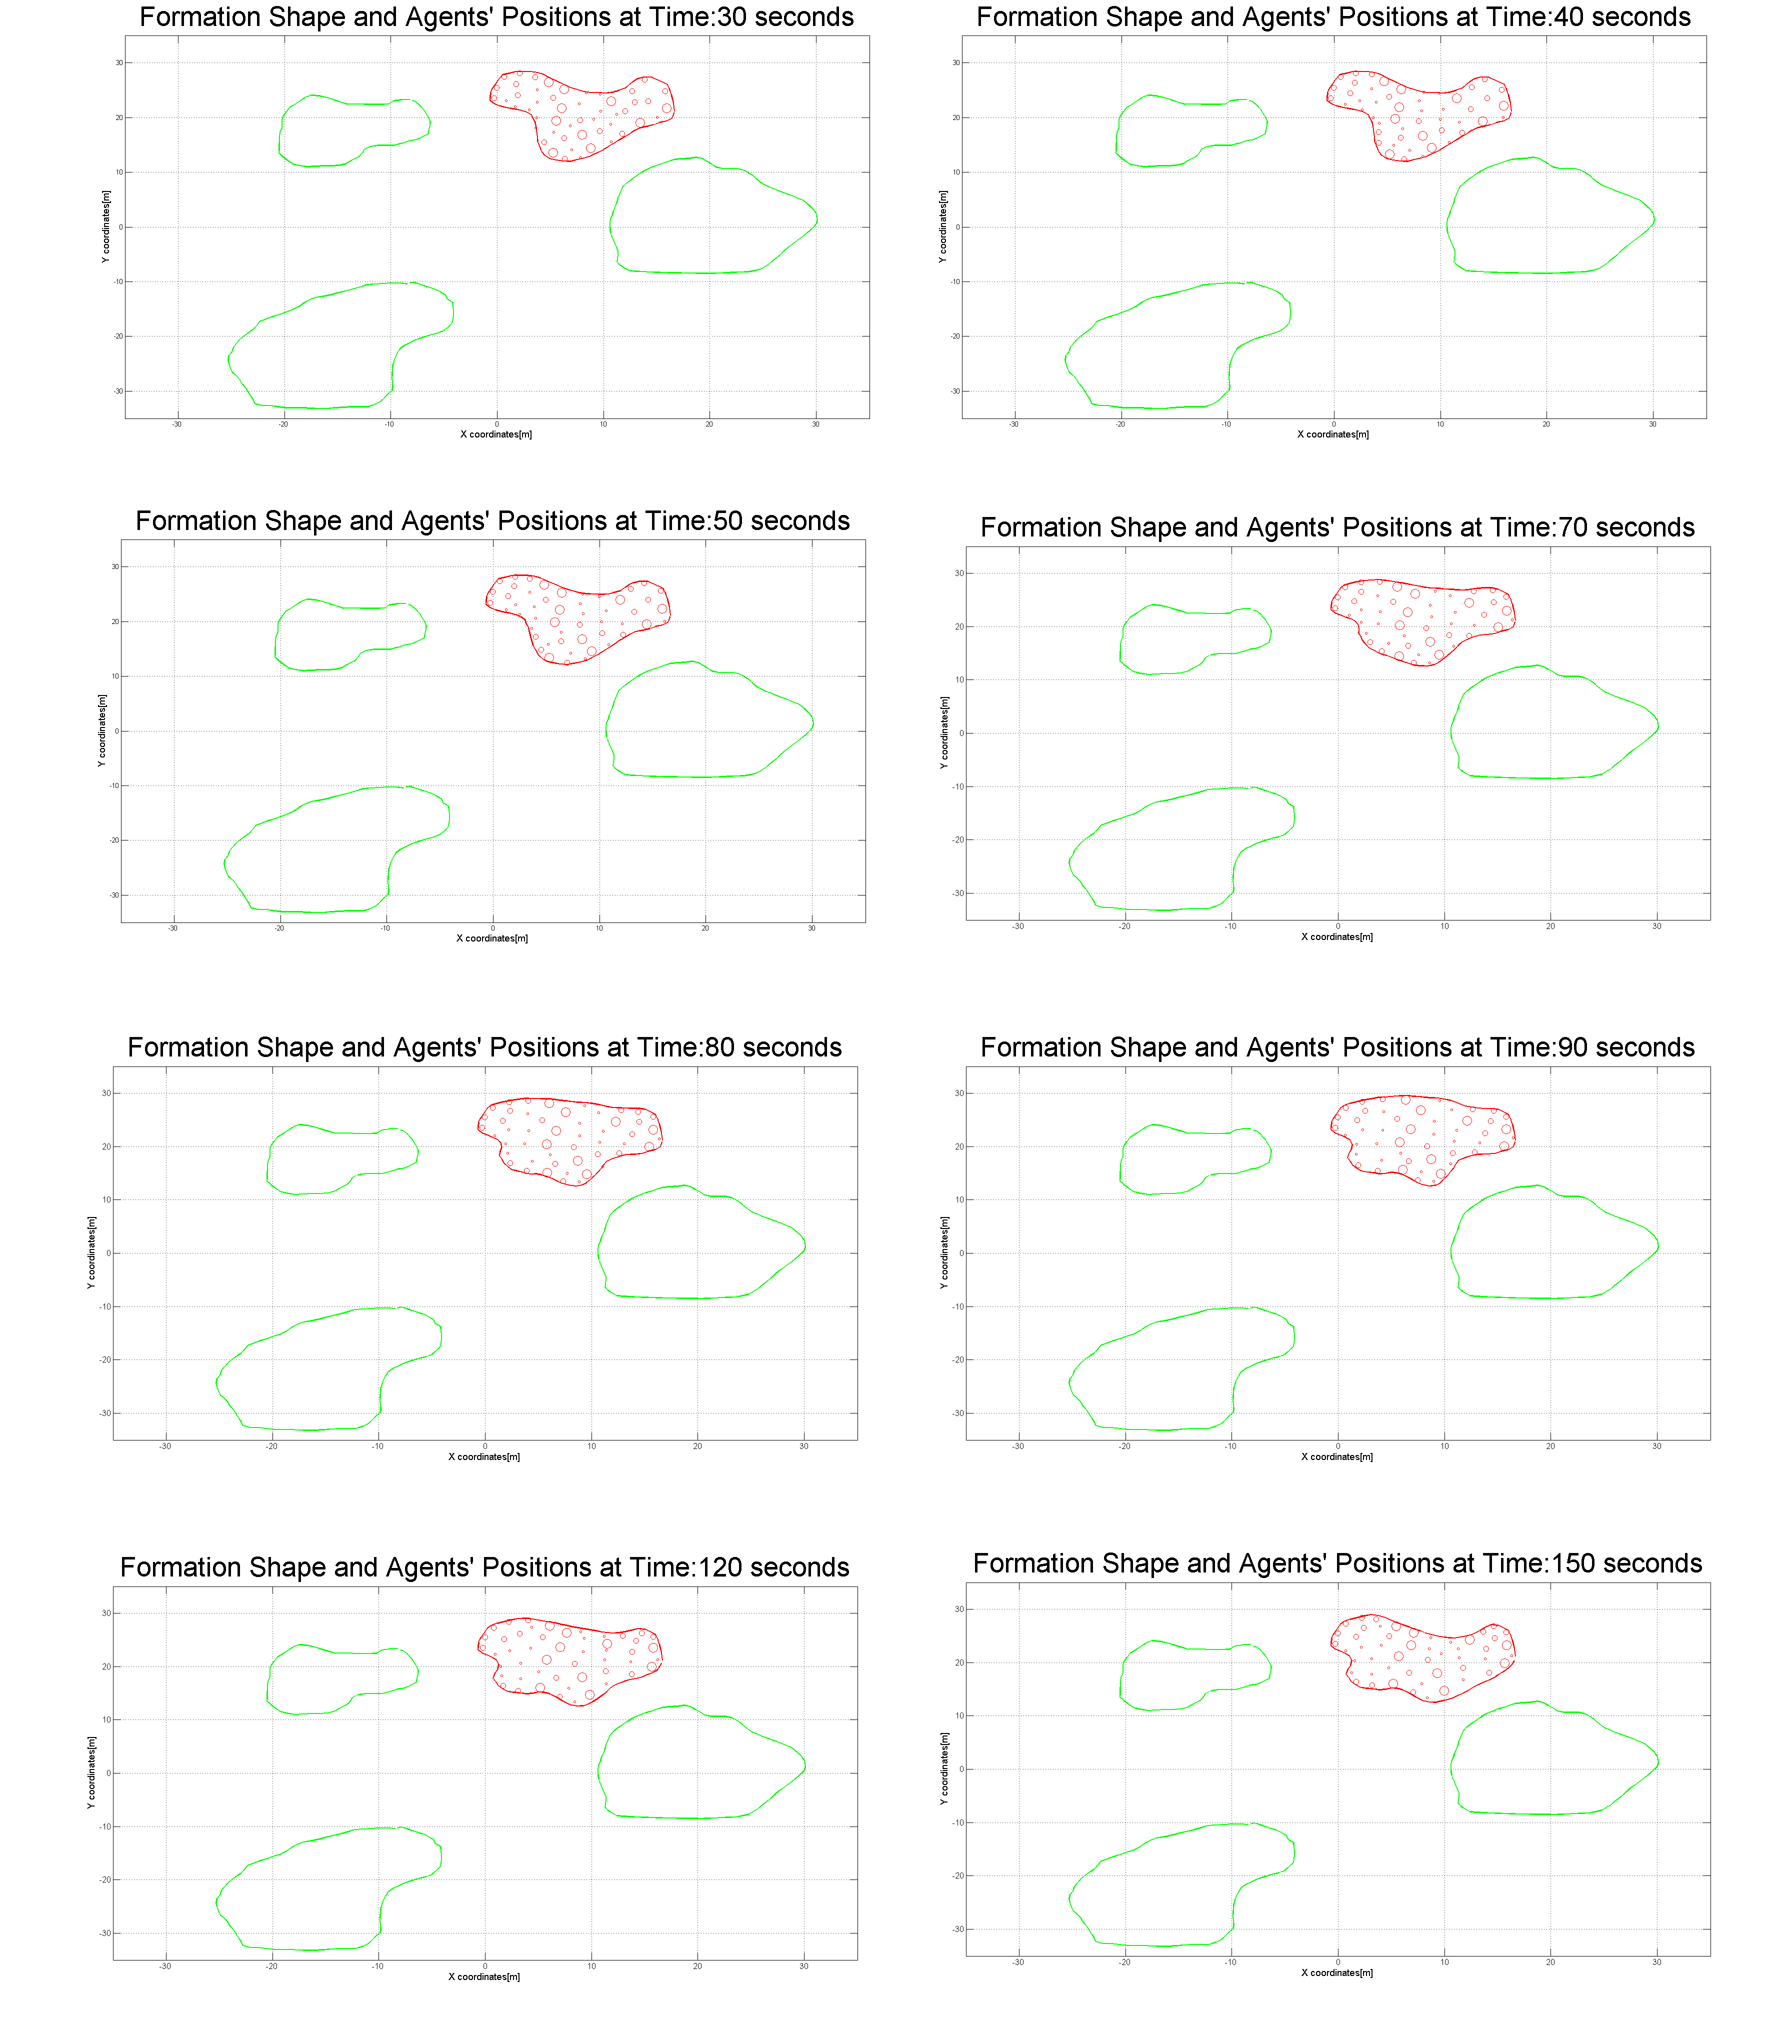
\includegraphics[scale = 0.16]{multiple1}}
\end{figure} 

Figure \ref{multiple1_ref} shows a simulation result for dynamical formation control implemented with Bubble Packing Method. Agents adapt themselves to the dynamically changing formation shape by assigning new positions of the goal states at each iterations. The positions of these goal states are determined with shape partitioning process implemented with Bubble Packing algorithm. 

\begin{figure}[H]
\caption{Dynamic Formation Control with Artificial Forces Method} \label{multiple2_ref}
\centerline{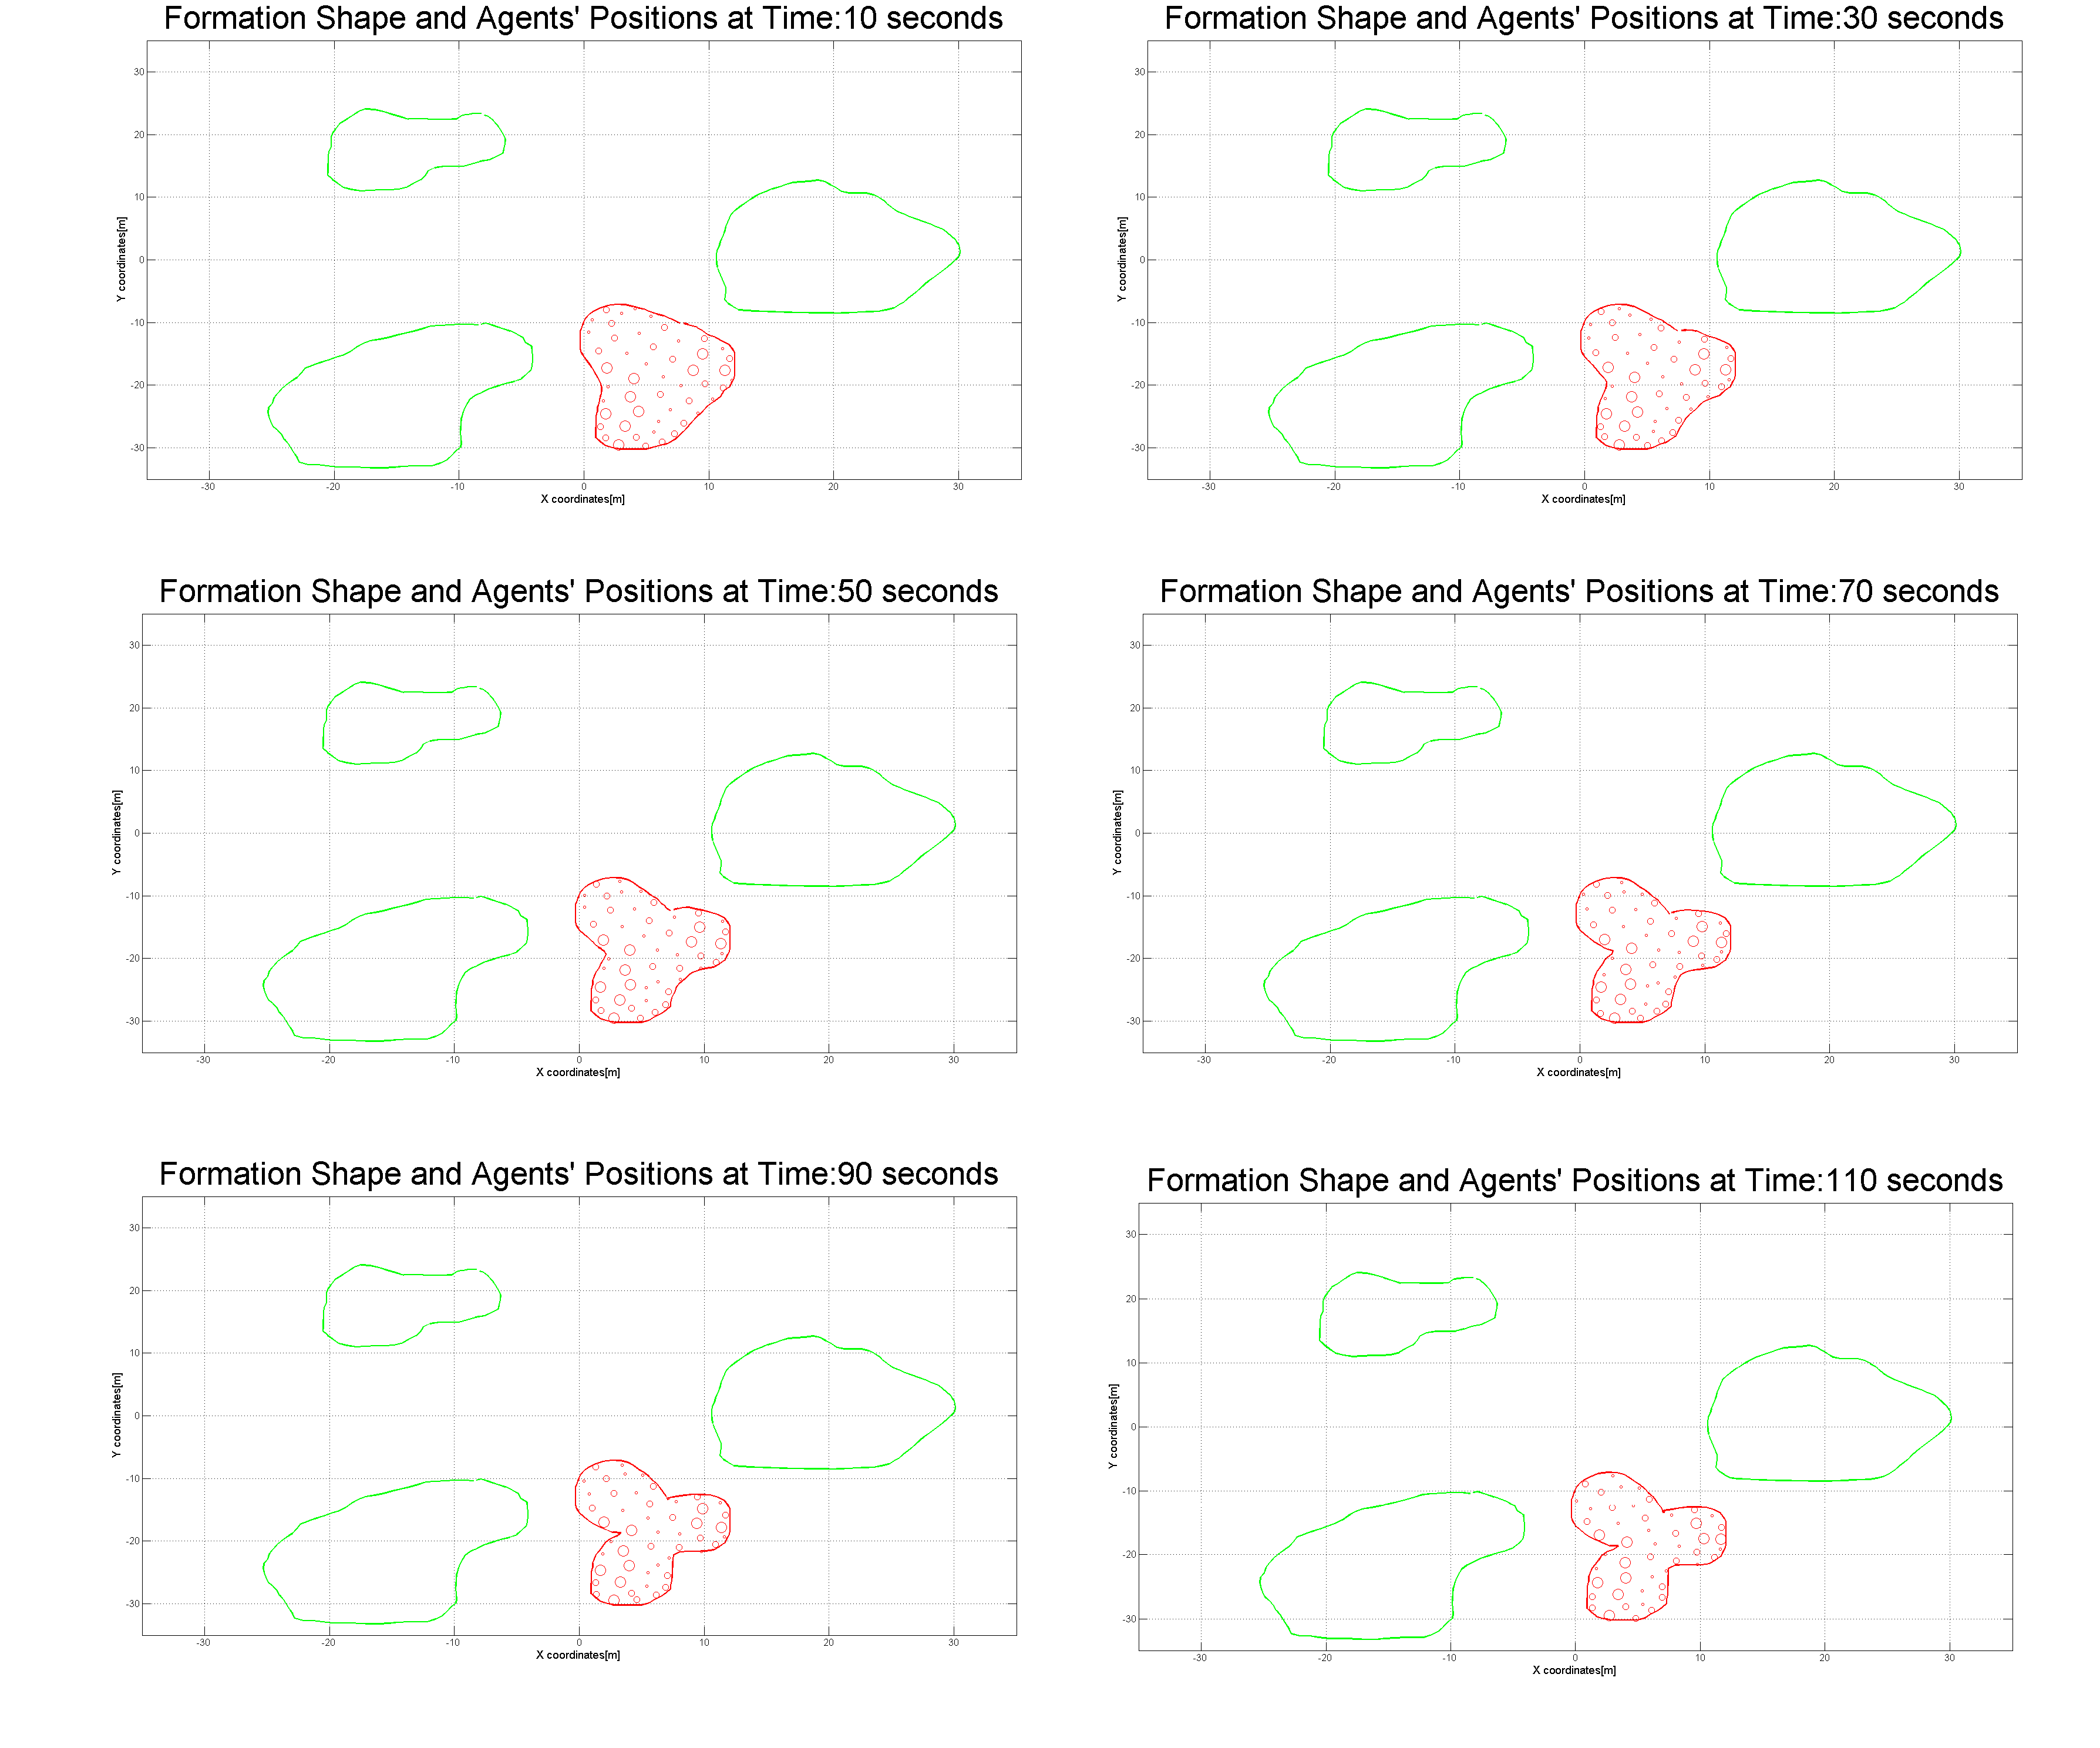
\includegraphics[scale = 0.16]{multiple2}}
\end{figure} 		 

Figure \ref{multiple2_ref} illustrates a simulation result of Artificial Forces method. In this method agents reposition in the changing formation shape with the help of artificial force components calculated with current formation shape. Since, agents directly adapts themselves to the changing formations shape in Artificial Forces method, it is expected to have a faster response than the Bubble Packing method. In Bubble Packing method, goal states are adapted to the changing formation shape and agents try to reach these goal states in runtime. This kind of approach introduces an additional latency to the response of the swarm to dynamically changing formation shapes. 

\begin{figure}[H]
\caption{Latency in Bubble Packing Method-1} \label{combo1_ref}
\centerline{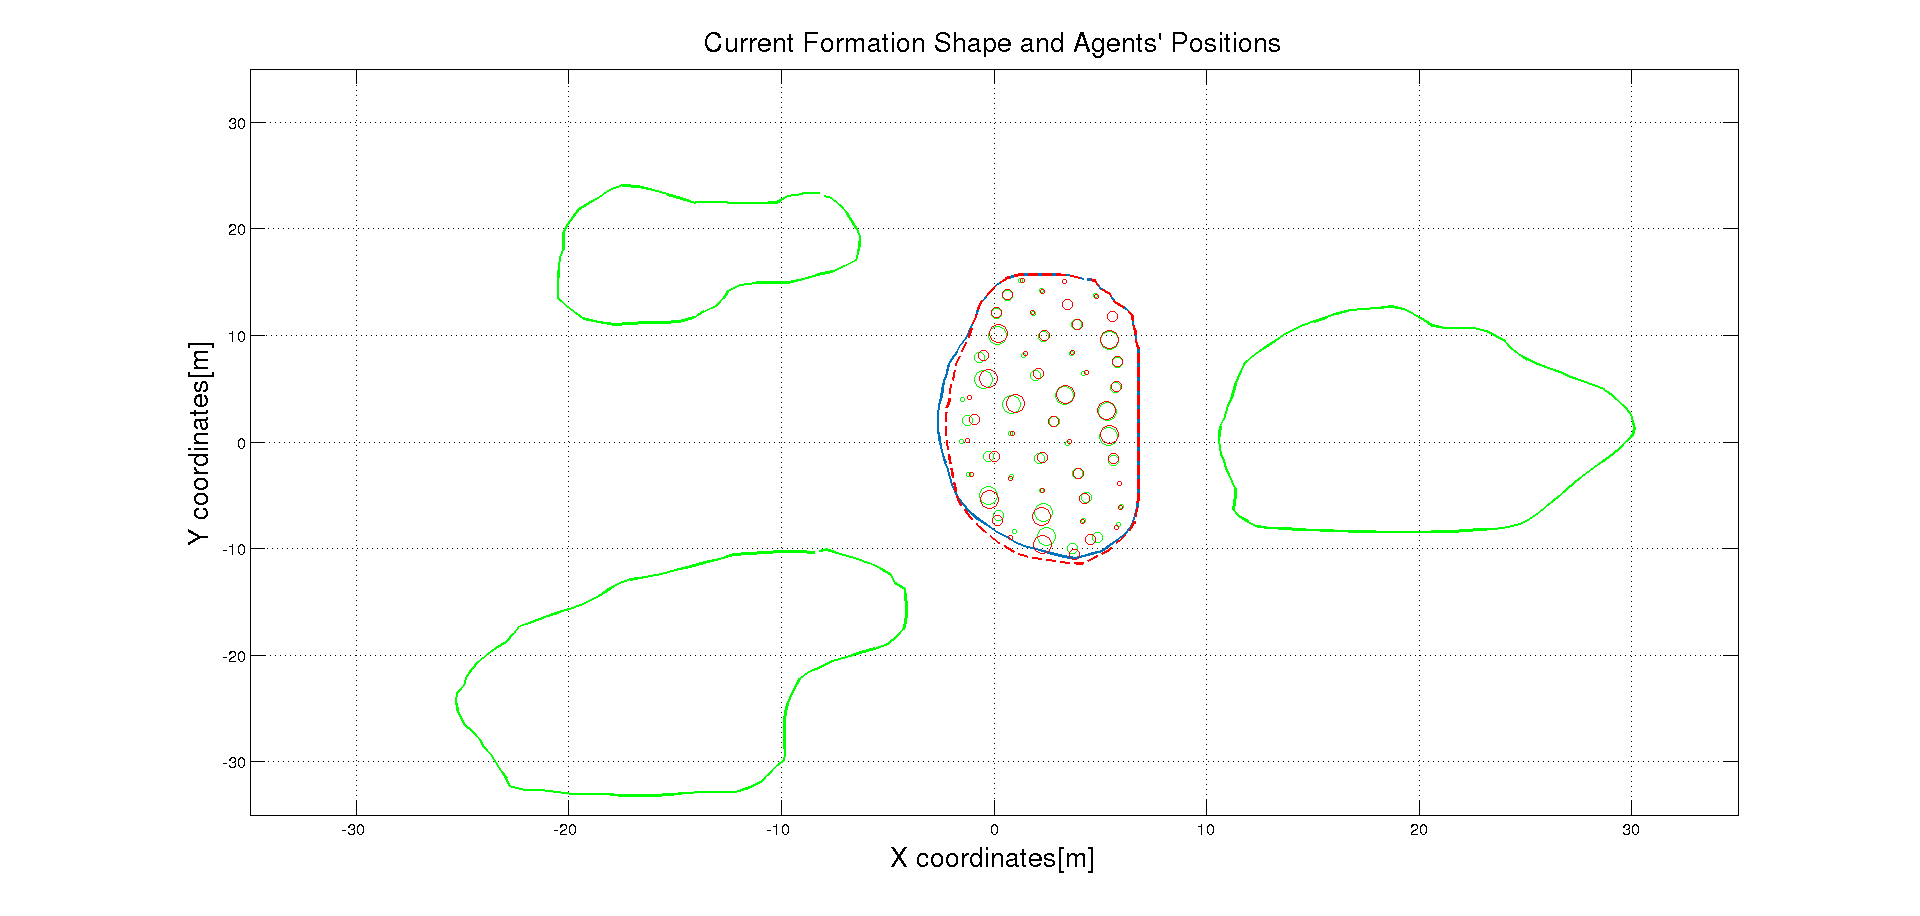
\includegraphics[scale = 0.30]{combo1}}
\end{figure} 

\begin{figure}[H]
\caption{Latency in Bubble Packing Method-2} \label{combo2_ref}
\centerline{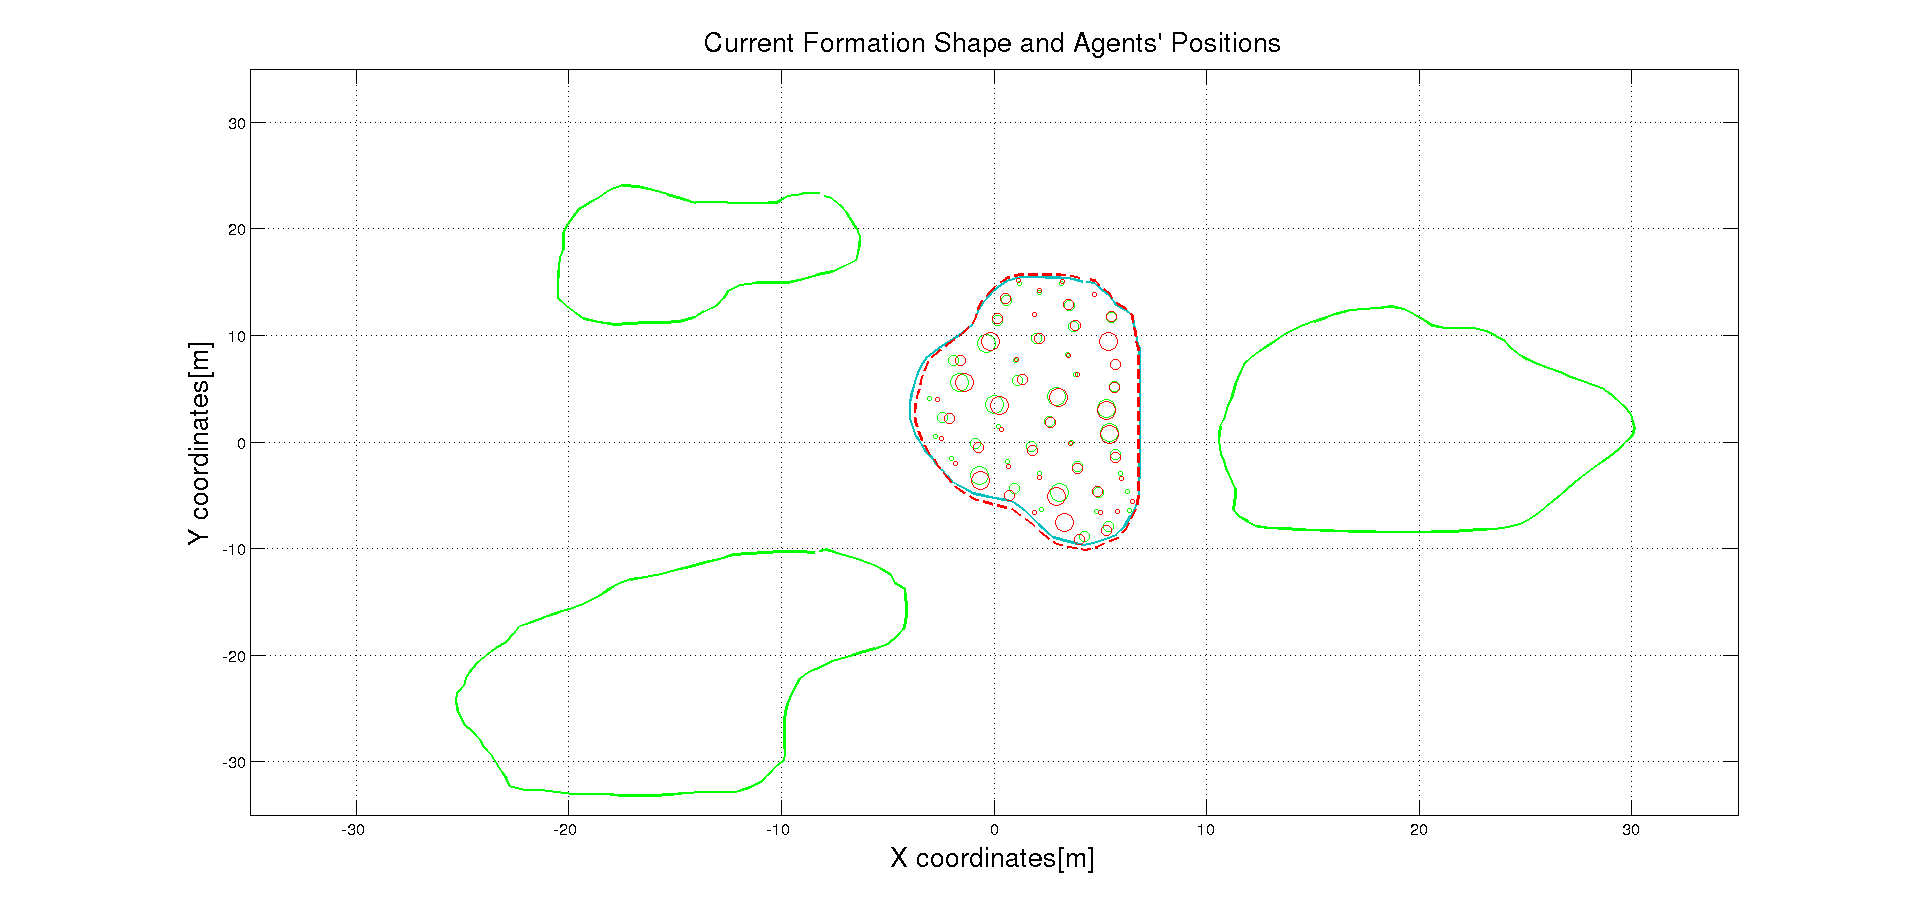
\includegraphics[scale = 0.30]{combo2}}
\end{figure} 

\begin{figure}[H]
\caption{Latency in Bubble Packing Method-3} \label{combo3_ref}
\centerline{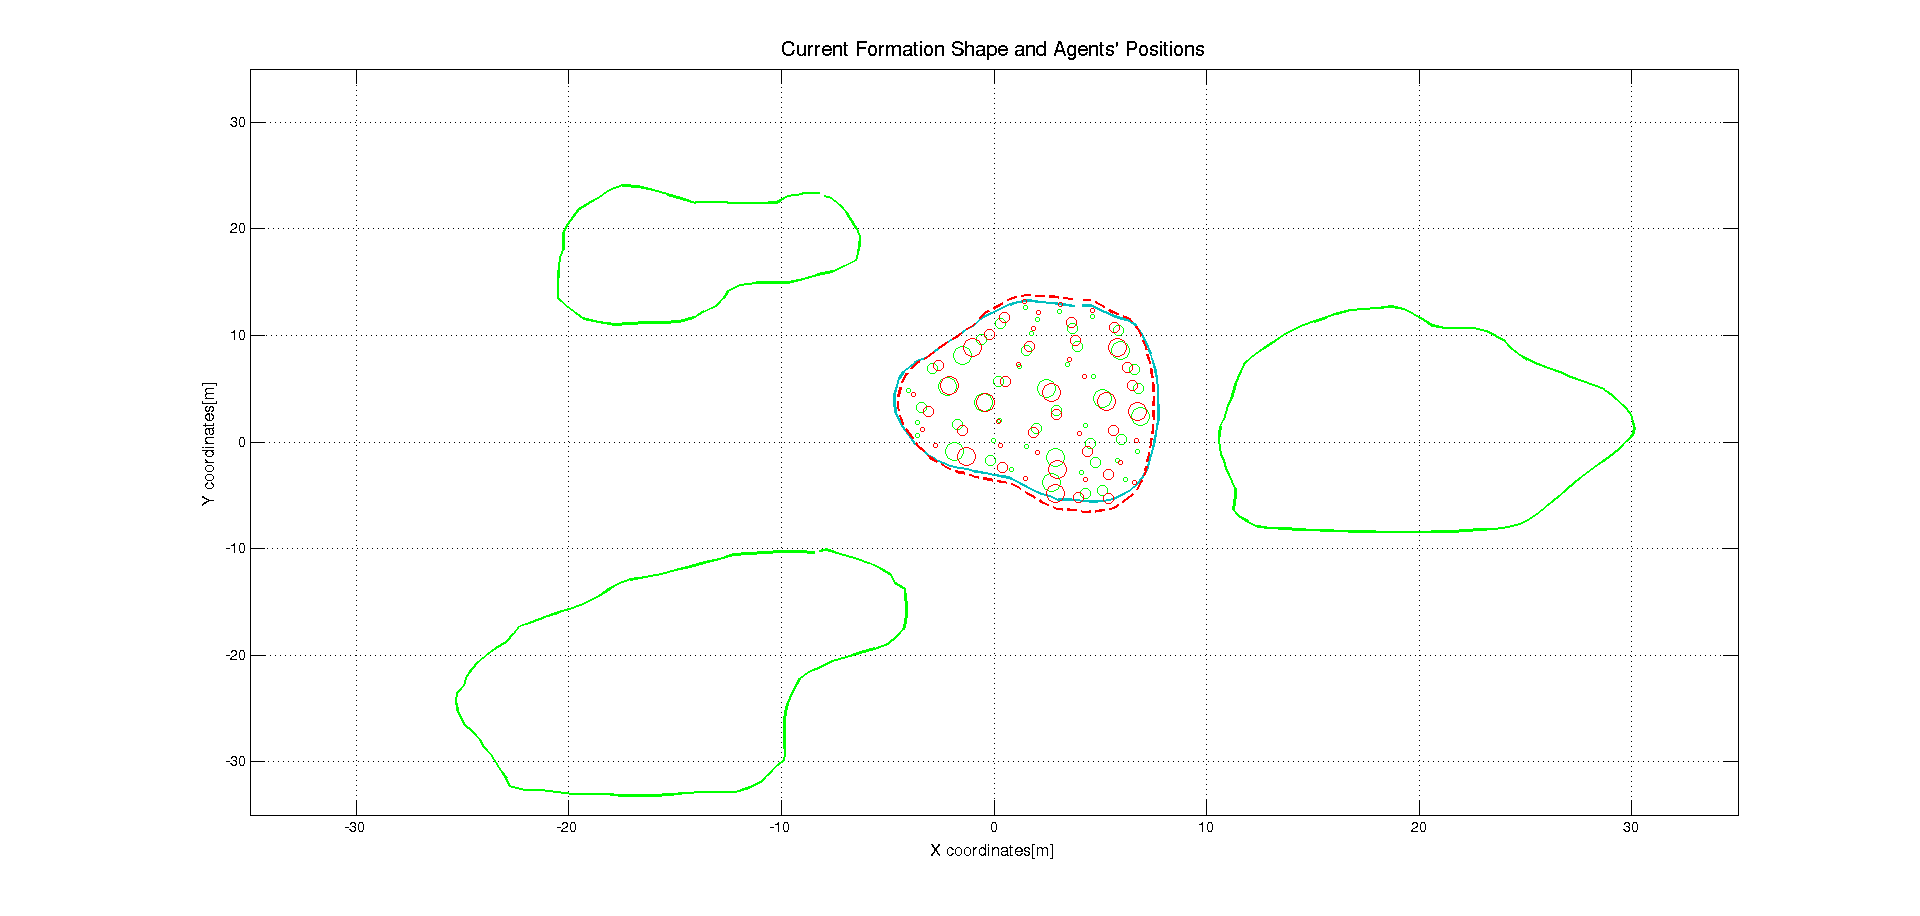
\includegraphics[scale = 0.30]{combo3}}
\end{figure} 

Figure \ref{combo1_ref}, \ref{combo2_ref} and \ref{combo3_ref} compares the responses of these two algorithms to dynamically changing formation shapes. Bubble Packing and Artificial Force algorithms are executed with the same dynamical formation shapes and same initial positions of the agents. In these figures, red circles are representing the agents' positions with Bubble Packing method and green circles are representing the agents' positions with Artificial Forces method at the same time from the beginning of the simulations. Formation shape with blue line illustrates the current formation shape. It is obvious that the green agents are adapted to the current formation shape better than the red ones. The shape with dotted red line, represents the estimated coverage area of red agents in the environment and this shape differs from the current formation shape locally at some boundary regions. This shows that agents response to the dynamically changing formation shape faster with Artifical Forces method. 

\subsection{Evaluation} \label{evaluation_ref}
Three different formation control approaches are evaluated with different kinds of metrics including the total displacement, settling time, mesh quality and dynamically changing formations. Artificial forces method has the worst performance in settling time and total displacement metrics due to the absence of predetermined goal states which is discussed in Section \ref{settling_ref} in details. On the other hand the Randomized Fractals method has the worst mesh quality performance because of its randomized nature of assignment the goal states in the desired formation shape. It is not possible to adapt the agents for dynamically changing formations with this method as discussed in Section \ref{dynamical_ref}. Artificial forces method has better response to the dynamically changing formations than the Bubble Packing method. The methods which have the worst performance at the related metrics are illustrated in Table \ref{worst_performance}
		
\begin{center}
\captionof{table}{Formation Control Methods with Worst Performance} \label{worst_performance} 
\begin{tabular}{||c| c| c | c | c||}
				
\hline
\textbf{Method/Metric} & \textbf{Total}  & \textbf{Settling} & \textbf{Mesh} & \textbf{Dynamical}\\ 
                       & \textbf{Displacement}  & \textbf{Time} & \textbf{Quality} & \textbf{Formation}\\
\hline
Artificial Force & X & X & & \\
Bubble Packing & &  & & X\\	
Randomized Fractals & &  & X & N/A \\	
\hline
\end{tabular}
\end{center}
		
It is obvious that Bubble Packing Method has the best performance for all metrics except for dynamical formation shapes. In fact, Bubble Packing method combines the efficient approaches of the other two methods. In the shape partitioning phase of the algorithm, it uses interbubble forces which have a similar structure with the intermember forces applied by the Artificial Forces method in formation control. This force has the greatest  effect on the homogeneity of the agents in the desired formation shape because it provides a global consensus for the agents in which each agent reaches an equilibrium state under the total force acting by their neighbors and the formation shape. On the other hand, Bubble Packing method implements an algorithm in which every agent is assigned to a goal state instantly at each execution period of the algorithm to minimize the overall displacement of the swarm. This approach reduce the settling time and the total displacements of the agents from the initial state to their final states since their final positions in the formation shape is predetermined. It is possible that the agents' goal states may be changed with the execution of the algorithm at different steps, but these assignments will converge to a unique subset while the agents are getting closer to the goal states. 

Artificial forces method has better performance on dynamically changing formations because it directly adapts the individual control signals on the agents according to the current formation shape. Bubble Packing method has a slower response to the dynamically changing formations due to its solution with two stages, shape partitioning and goal state assignment. 
		
We have made some different formation shape trials by using these different methods. Following figures and tables, illustrates these trials and their performance metrics.

\begin{figure}[H]
\caption{Formation Shape - 1 in Gazebo Environment}
\centerline{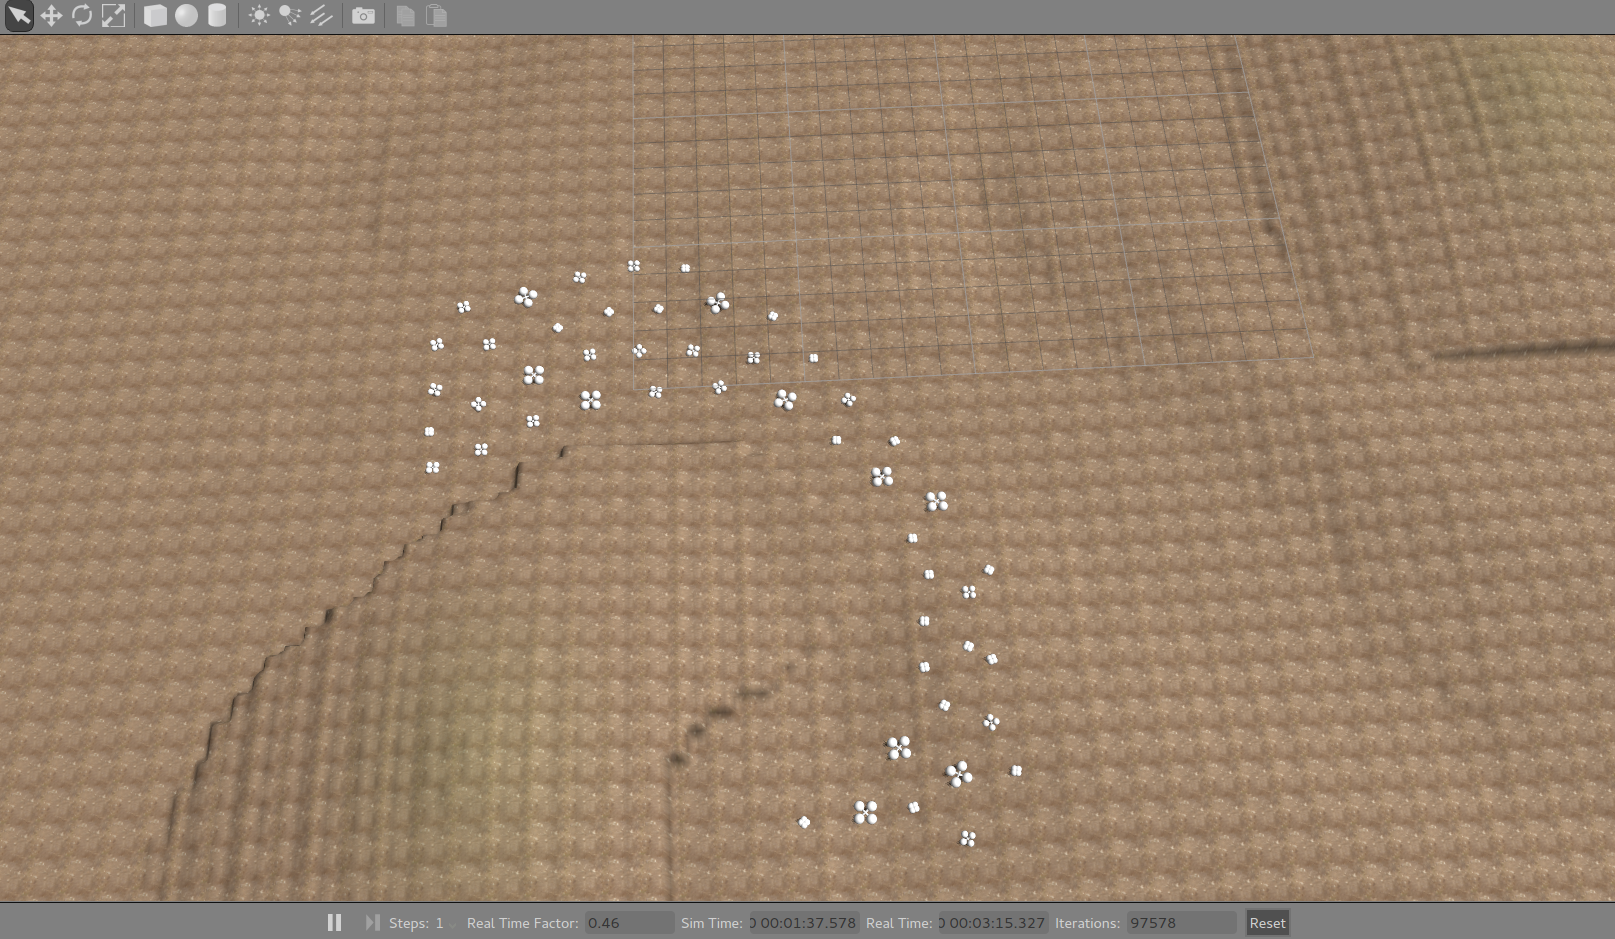
\includegraphics[scale = 0.32]{1_Gazebo}}
\end{figure} 
			
\begin{figure}[H]
\caption{Formation Shape - 1 in MATLAB Environment}
\centerline{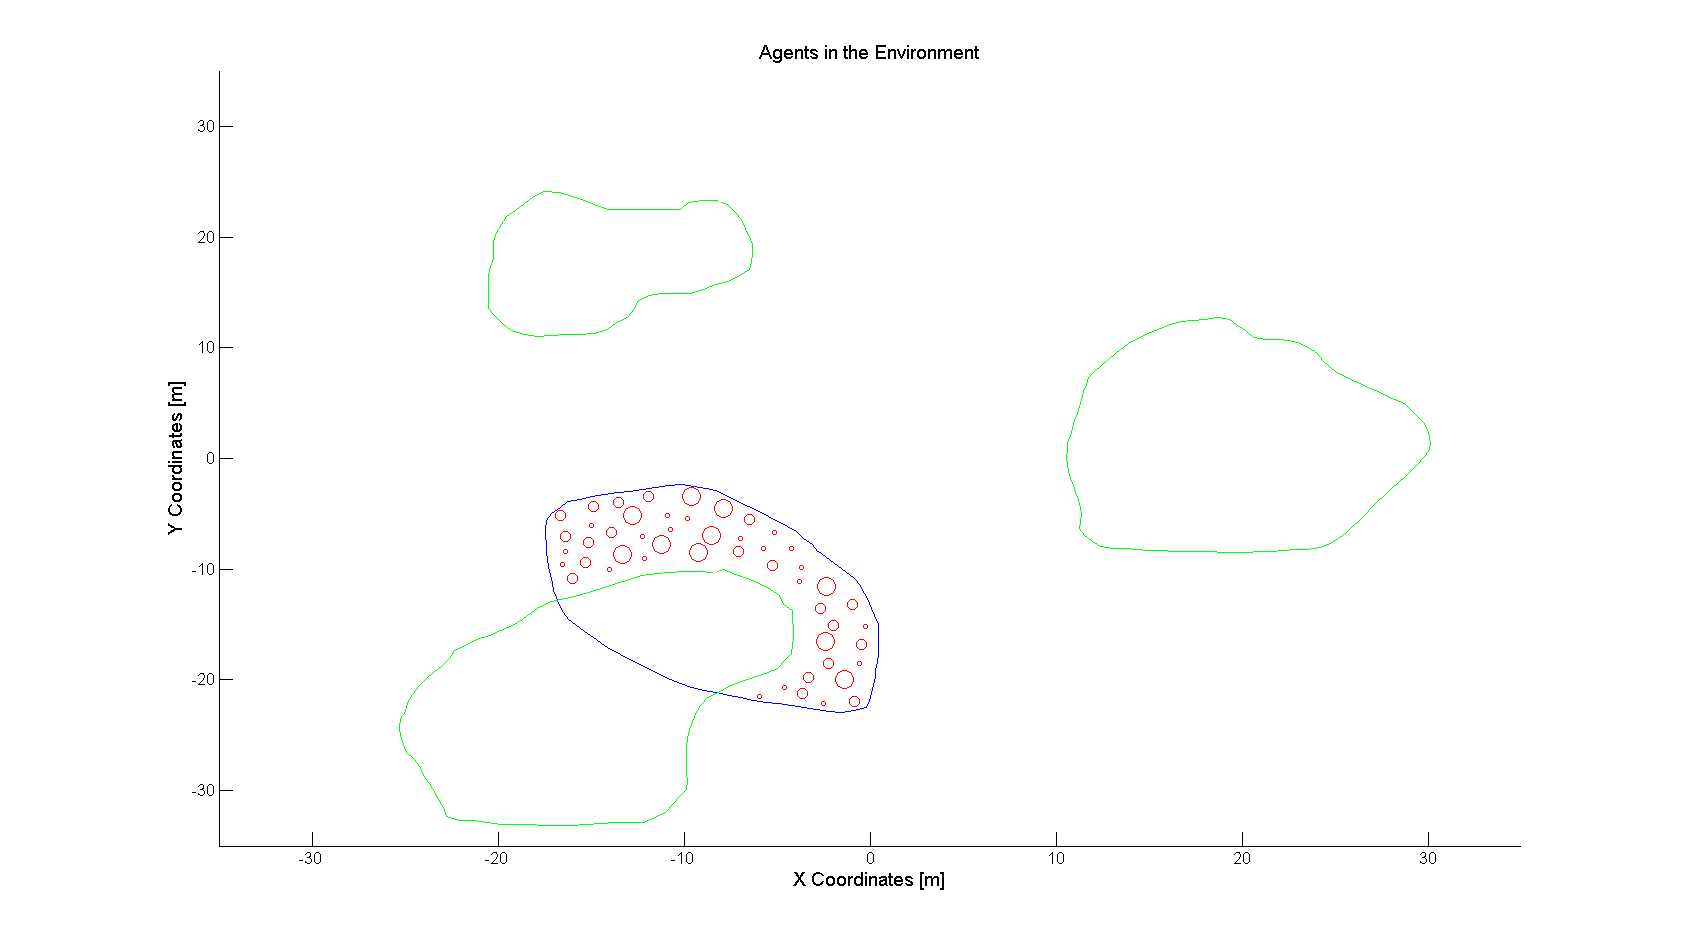
\includegraphics[scale = 0.32]{1}}
\end{figure} 
			
\begin{center}
\captionof{table}{Performance Metrics for Shape - 1} \label{perf_shape1} 
\begin{tabular}{|c|c|c|c|c|}
					
\hline
\textbf{} & \textbf{Total}  & \textbf{Total Settling} & \textbf{} & \textbf{} \\ \textbf{Method} & \textbf{Displacement[m]} & \textbf{Time[sec]}& \textbf{$\epsilon_t$} & \textbf{$\epsilon_g$} \\
\hline
Artificial&  &  &  & \\
 Forces & 1889 & 164& 2.54 & 0.62\\
 \hline
 Bubble&  &  &  & \\
 Packing &1750 &151 &2.44 & 0.67\\
\hline
 Randomized&  &  &  & \\
 Fractals &1762 &153 &3.14 & 0.92\\
\hline
\end{tabular}
\end{center}
	
\begin{figure}[H]
\caption{Formation Shape - 2 in Gazebo Environment}
\centerline{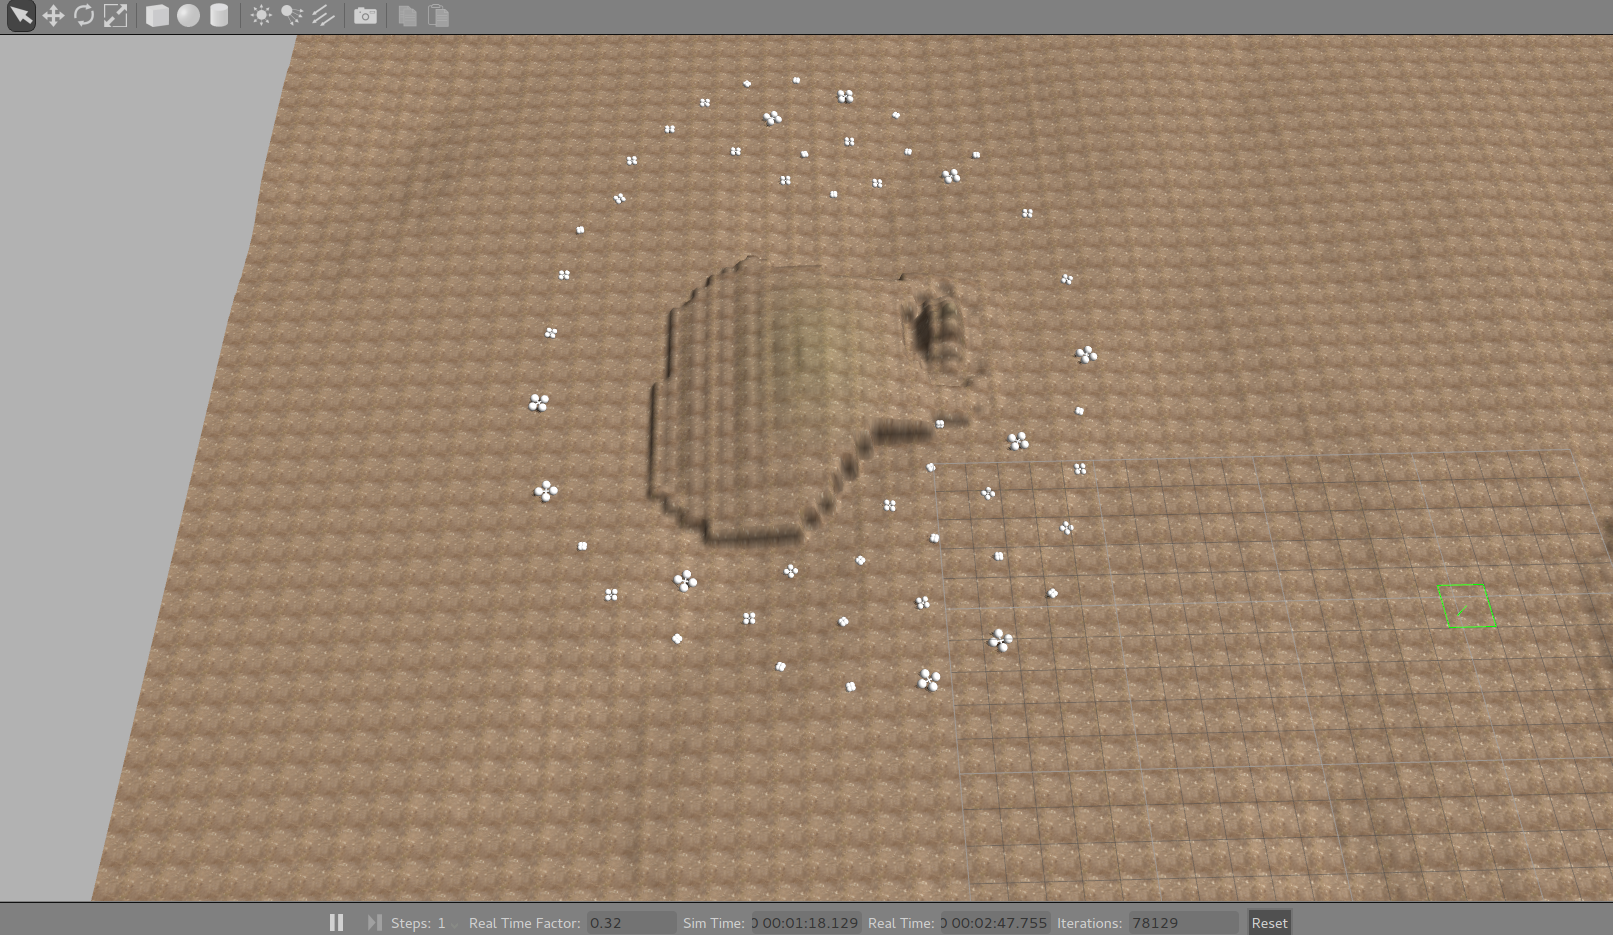
\includegraphics[scale = 0.32]{2_Gazebo}}
\end{figure} 
		 
\begin{figure}[H]
\caption{Formation Shape - 2 in MATLAB Environment}
\centerline{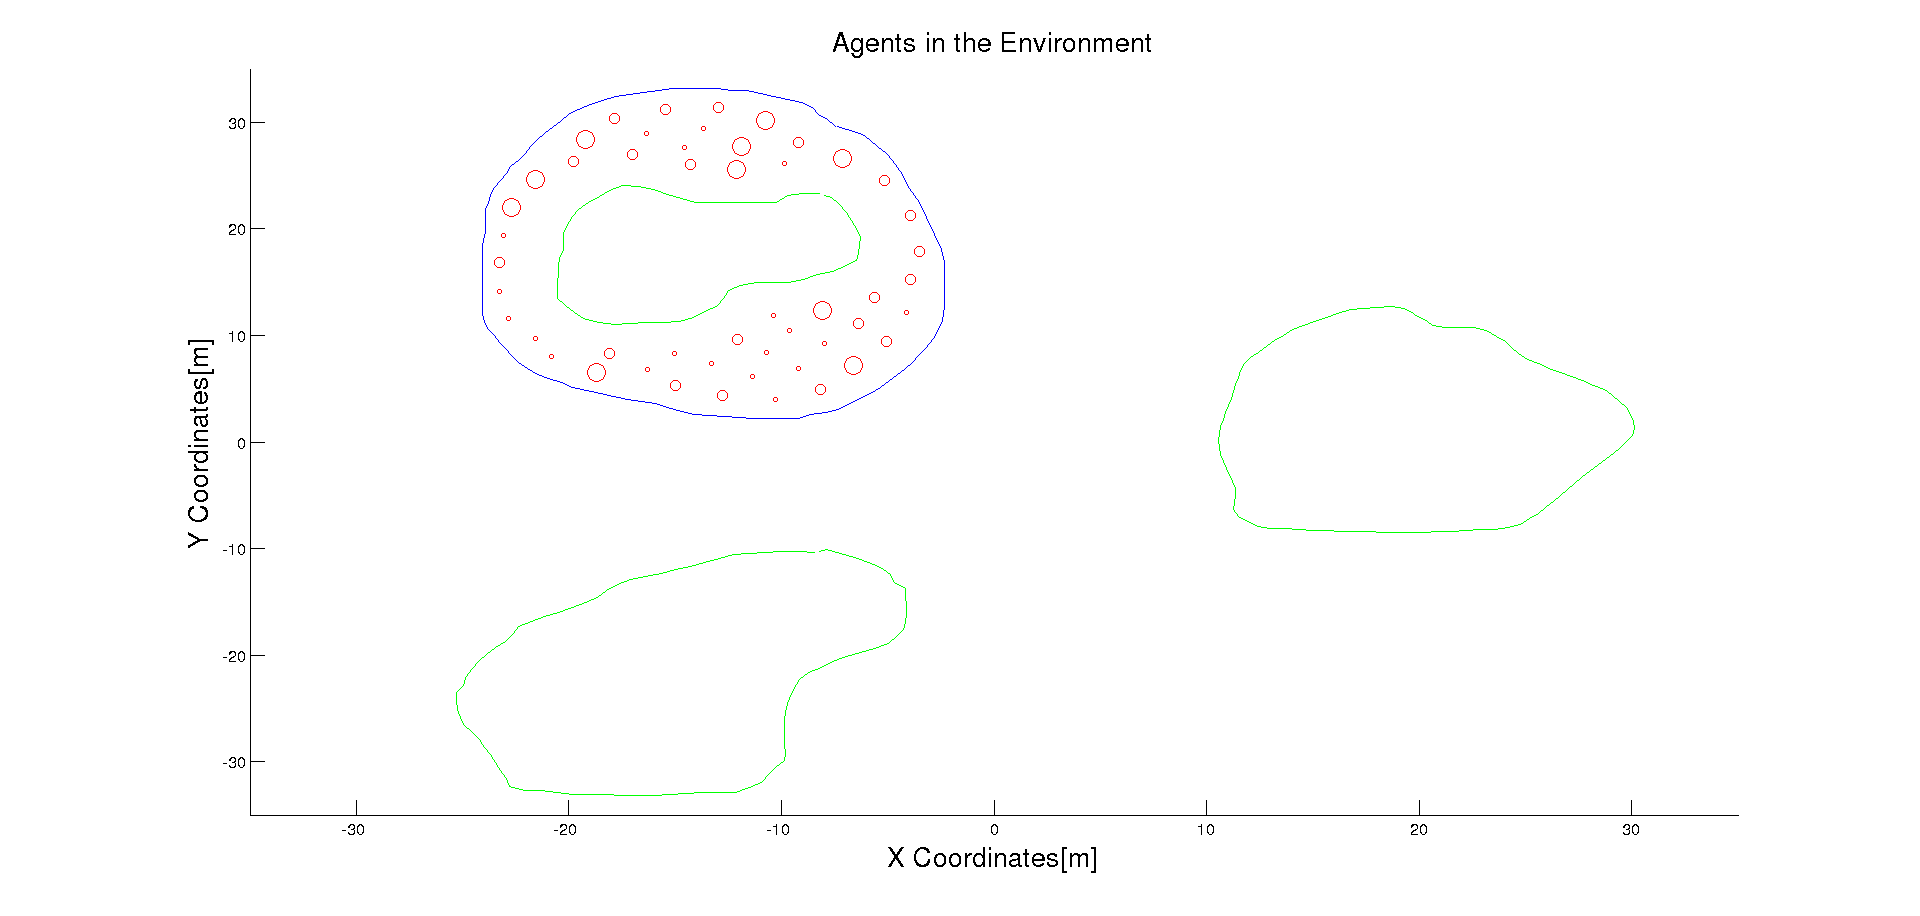
\includegraphics[scale = 0.32]{2}}
\end{figure} 
		 

		 
\begin{center}
\captionof{table}{Performance Metrics for Shape - 2} \label{perf_shape2} 
\begin{tabular}{|c|c|c|c|c|}
					
\hline
\textbf{} & \textbf{Total}  & \textbf{Total Settling} & \textbf{} & \textbf{} \\ \textbf{Method} & \textbf{Displacement[m]} & \textbf{Time[sec]}& \textbf{$\epsilon_t$} & \textbf{$\epsilon_g$} \\
\hline
Artificial&  &  &  & \\
 Forces & 1611 & 153& 2.95 & 0.73\\
 \hline
 Bubble&  &  &  & \\
 Packing &1550 &141 &2.84 & 0.77\\
\hline
 Randomized&  &  &  & \\
 Fractals &1522 &140 &3.24 & 1.12\\
\hline
\end{tabular}
\end{center}
		 		

		 
\begin{figure}[H]
\caption{Formation Shape - 3 in Gazebo Environment}
\centerline{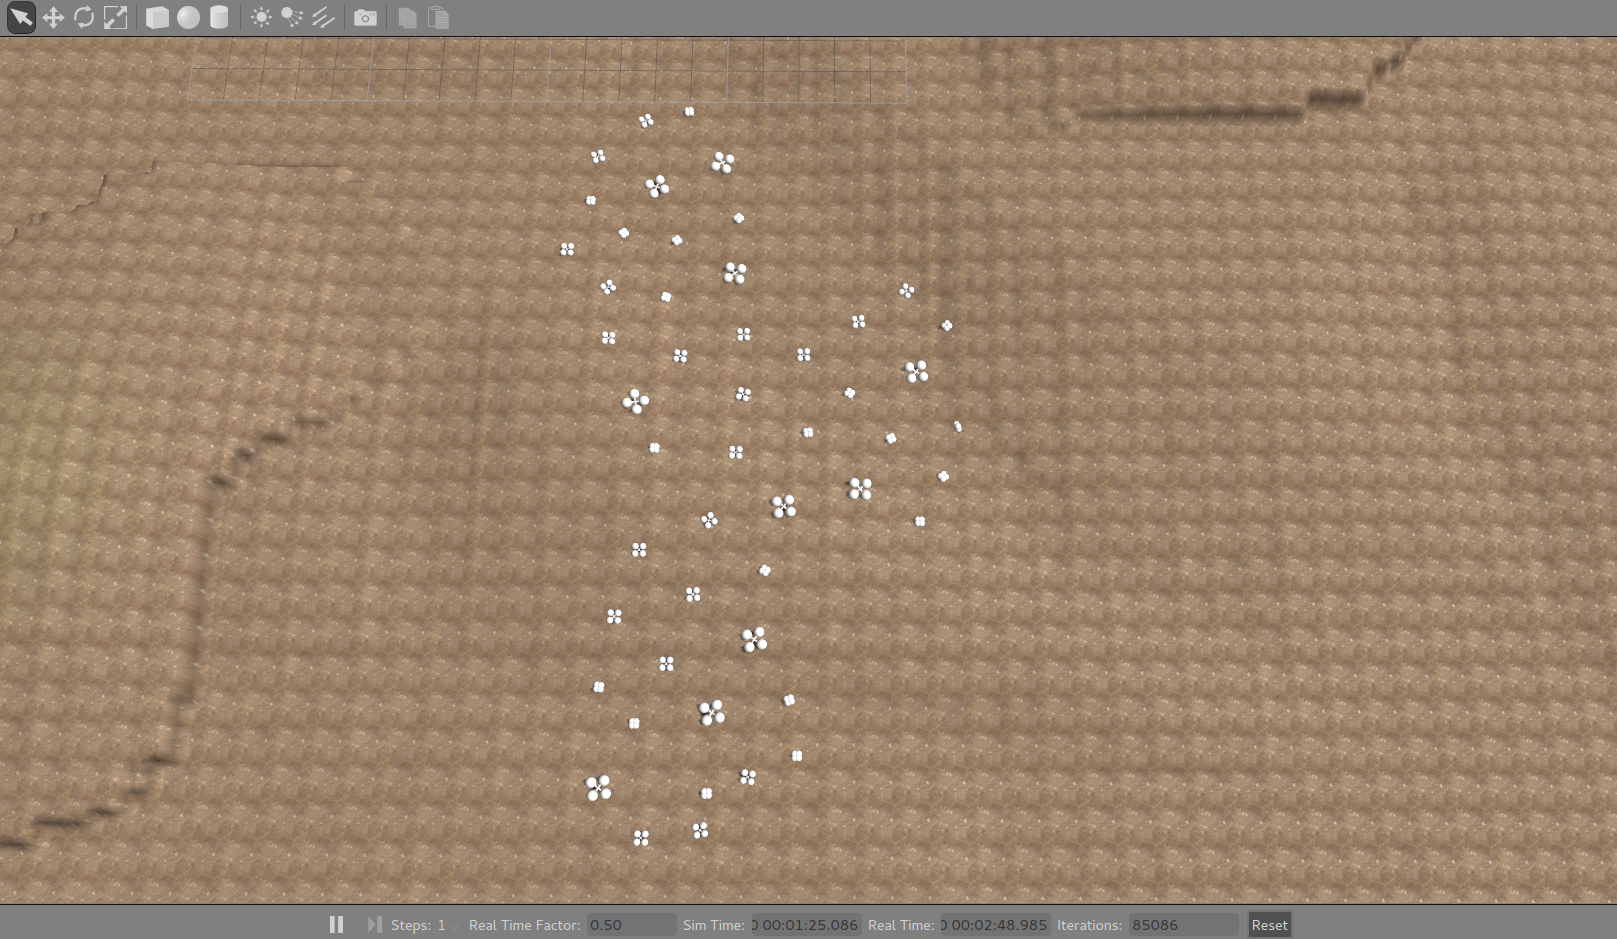
\includegraphics[scale = 0.32]{3_Gazebo}}
\end{figure} 
				 
\begin{figure}[H]
\caption{Formation Shape - 3 in MATLAB Environment}
\centerline{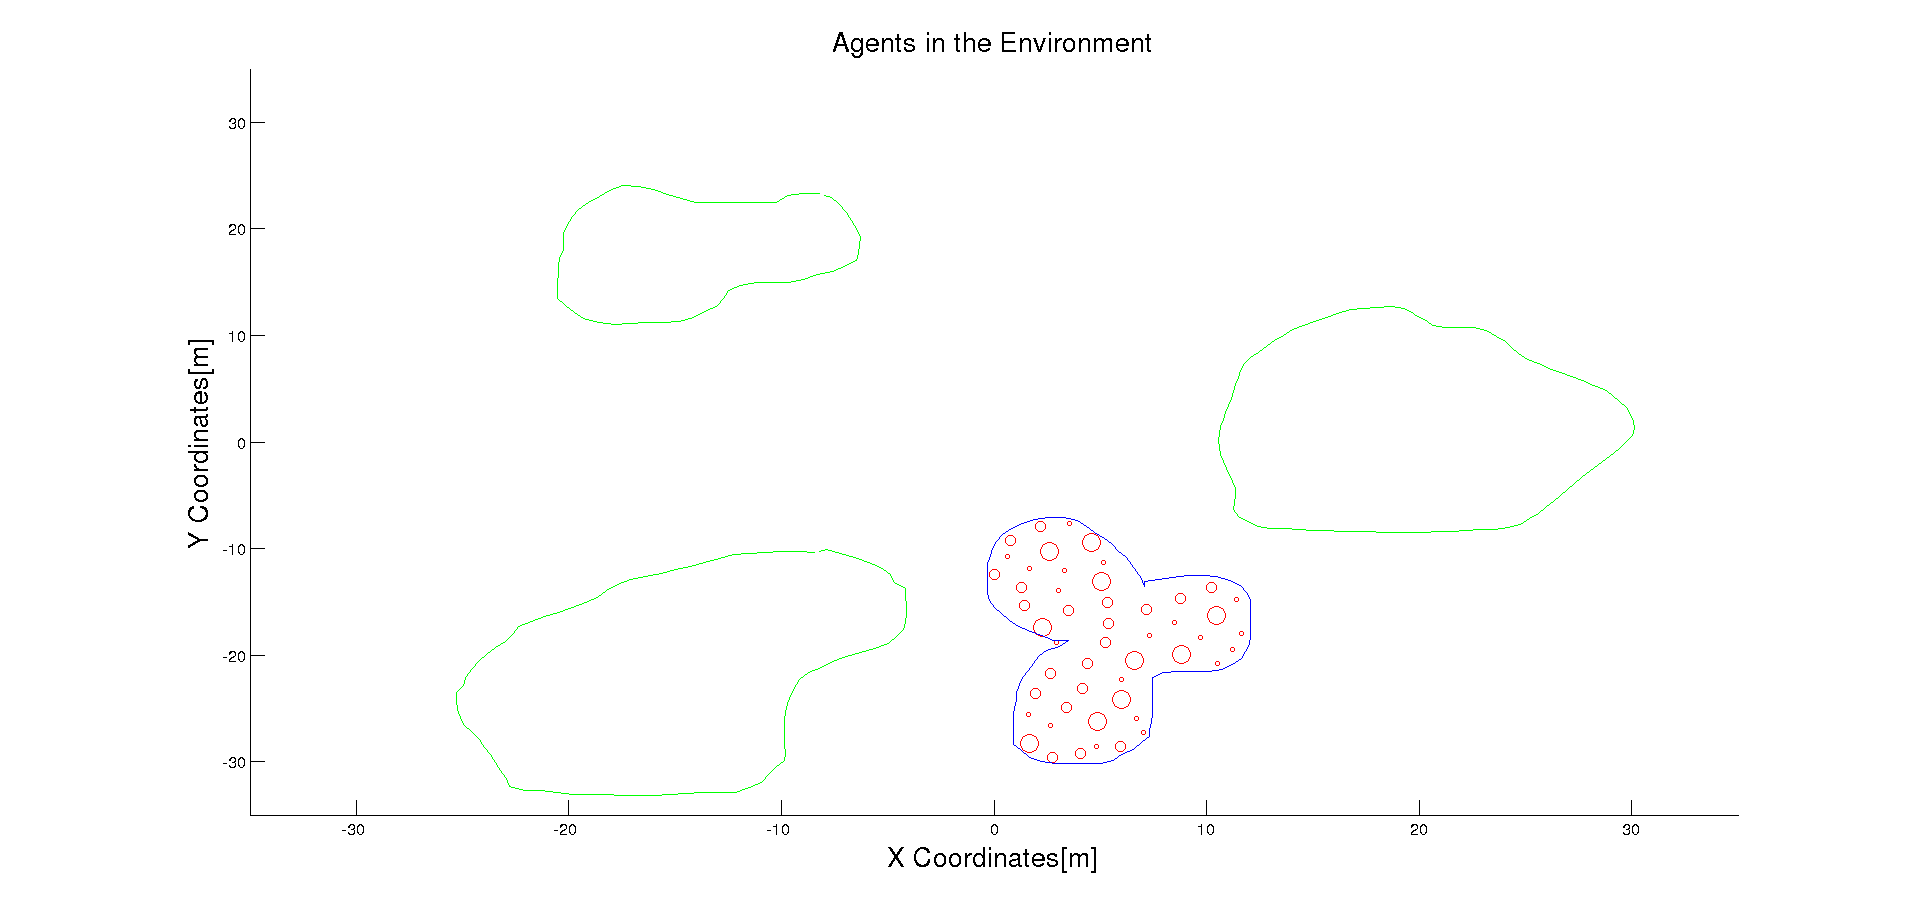
\includegraphics[scale = 0.32]{3}}
\end{figure} 
				 

			
			
\begin{center}
\captionof{table}{Performance Metrics for Shape - 3} \label{perf_shape3} 
\begin{tabular}{|c|c|c|c|c|}
					
\hline
\textbf{} & \textbf{Total}  & \textbf{Total Settling} & \textbf{} & \textbf{} \\ \textbf{Method} & \textbf{Displacement[m]} & \textbf{Time[sec]}& \textbf{$\epsilon_t$} & \textbf{$\epsilon_g$} \\
\hline
Artificial&  &  &  & \\
 Forces & 1432 & 126& 2.23 & 0.45\\
 \hline
 Bubble&  &  &  & \\
 Packing &1330 &115 &2.14 & 0.52\\
\hline
 Randomized&  &  &  & \\
 Fractals &1350 &112 &3.15 & 0.89\\
\hline
\end{tabular}
\end{center}

				 
\begin{figure}[H]
\caption{Formation Shape - 4 in Gazebo Environment}
\centerline{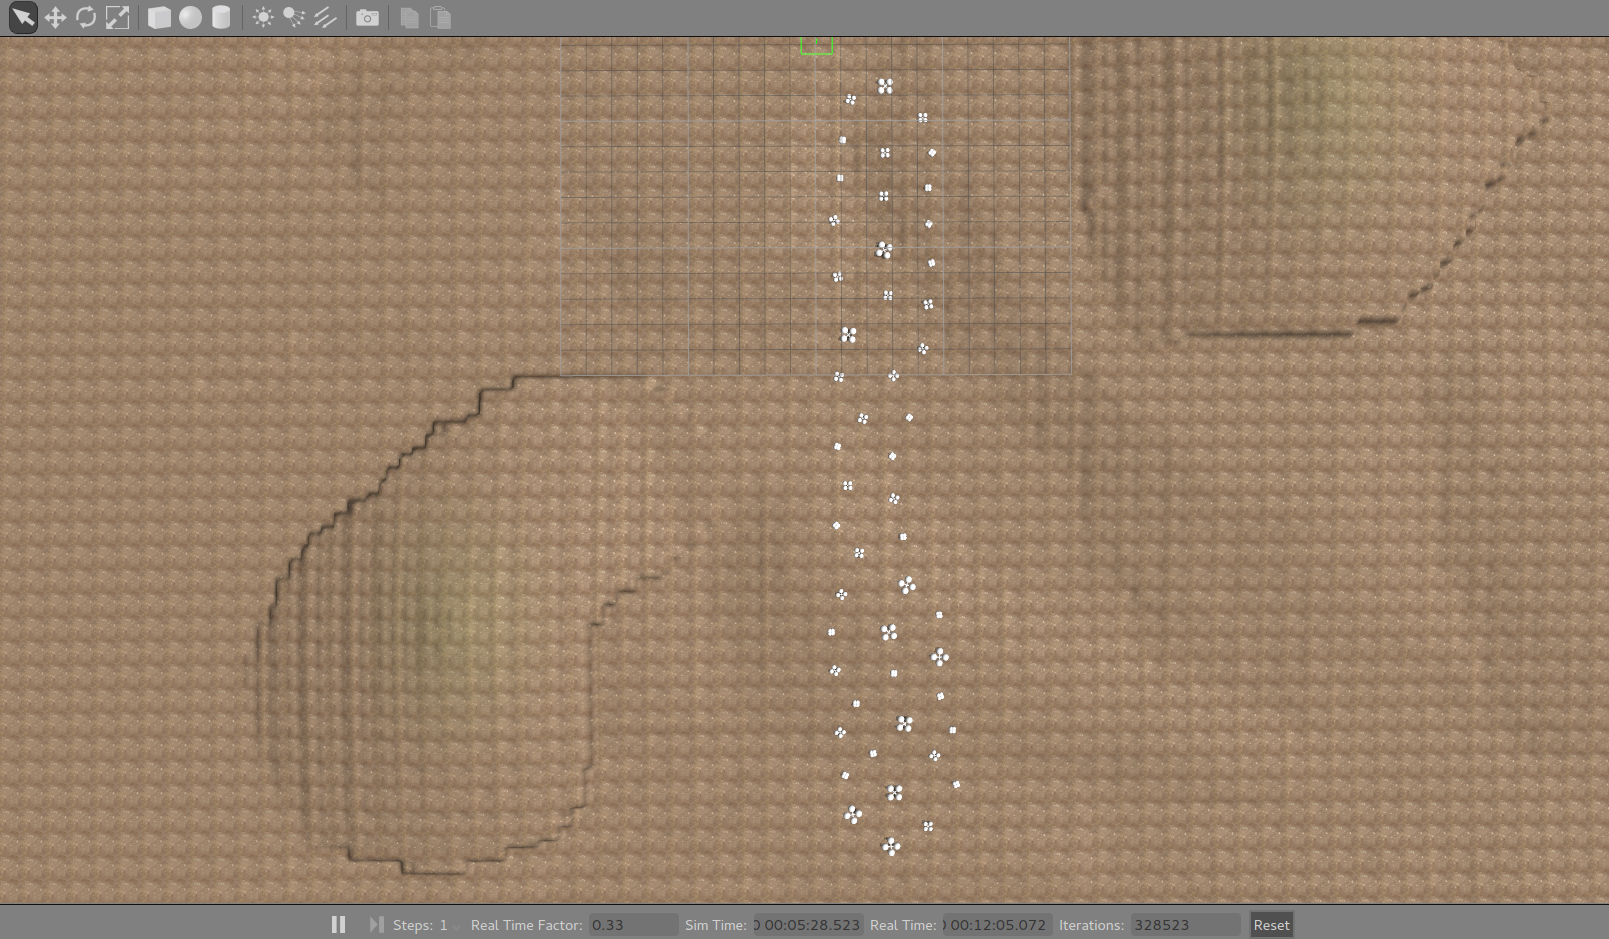
\includegraphics[scale = 0.32]{4_Gazebo}}
\end{figure} 
			
\begin{figure}[H]
\caption{Formation Shape - 4 in MATLAB Environment}
\centerline{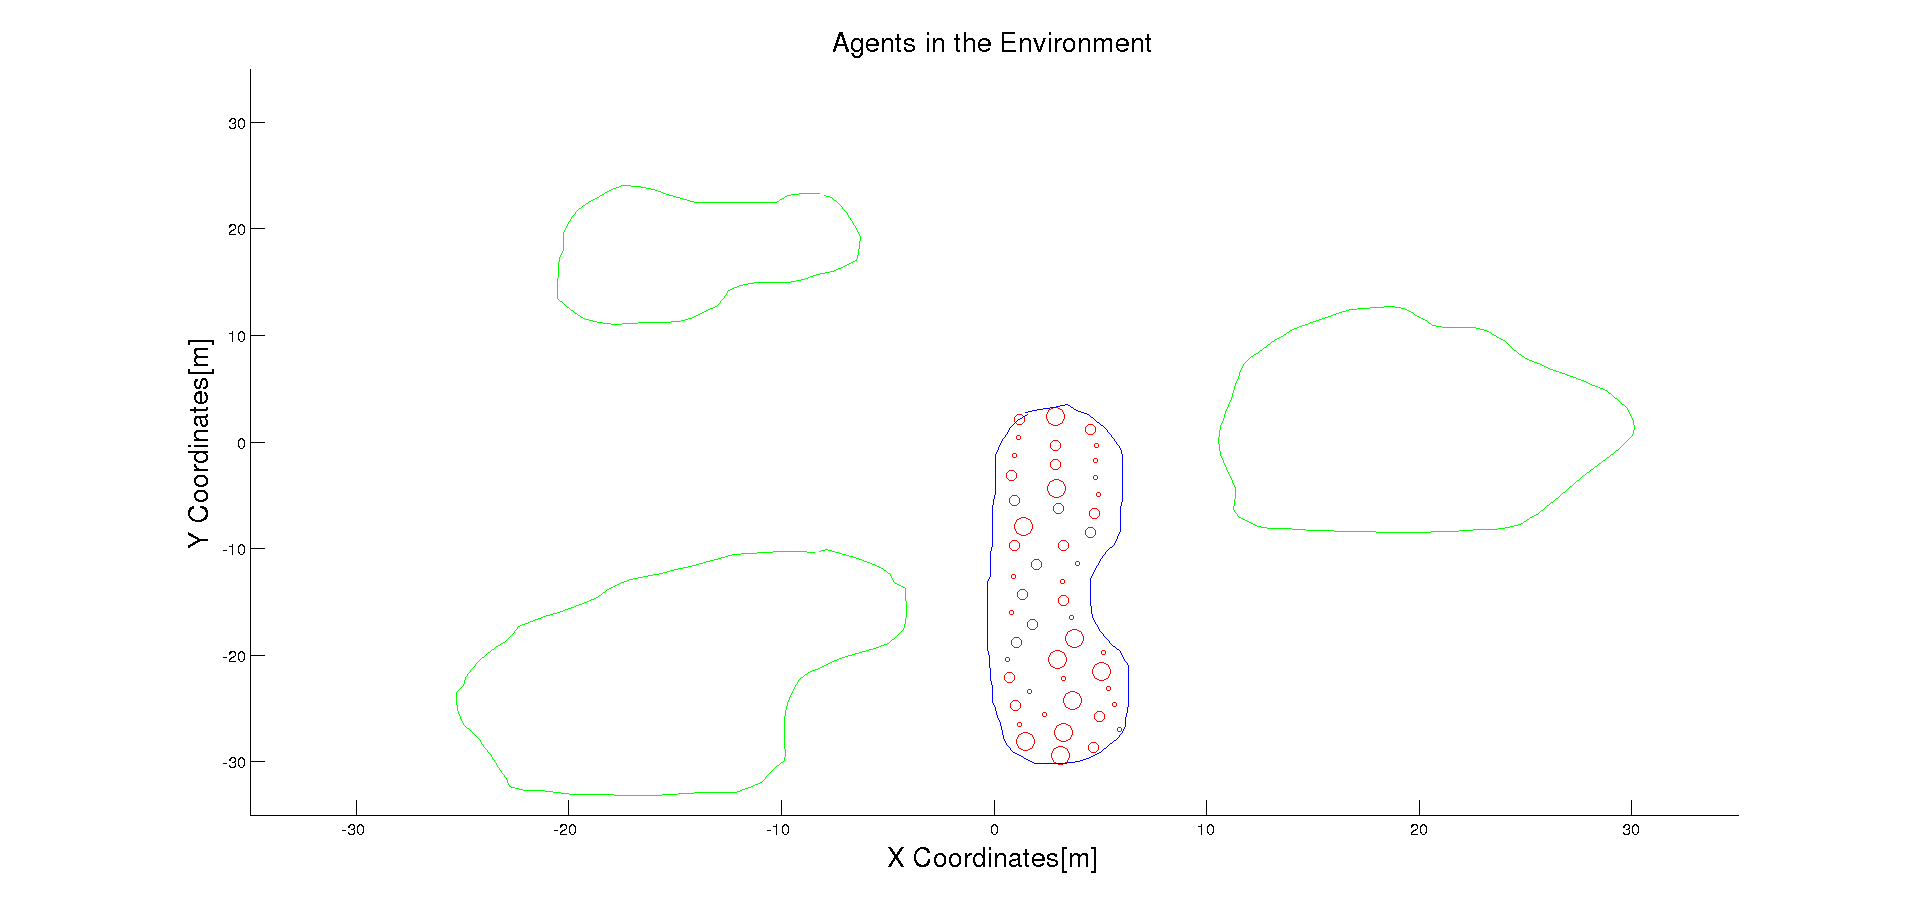
\includegraphics[scale = 0.32]{4}}
\end{figure} 
			
	
\begin{center}
\captionof{table}{Performance Metrics for Shape - 4} \label{perf_shape4} 
\begin{tabular}{|c|c|c|c|c|}
					
\hline
\textbf{} & \textbf{Total}  & \textbf{Total Settling} & \textbf{} & \textbf{} \\ \textbf{Method} & \textbf{Displacement[m]} & \textbf{Time[sec]}& \textbf{$\epsilon_t$} & \textbf{$\epsilon_g$} \\
\hline
Artificial&  &  &  & \\
 Forces & 1578 & 142& 2.15 & 0.56\\
 \hline
 Bubble&  &  &  & \\
 Packing &1345 &112 &2.34 & 0.66\\
\hline
 Randomized&  &  &  & \\
 Fractals &1321 &121 &3.23 & 1.05\\
\hline
\end{tabular}
\end{center}
		
A simulation with multiple formation shapes sequentially is illustrated in Figure \ref{multiple_formation_ref}.

\begin{figure}[H]
\caption{Multiple Formations} \label{multiple_formation_ref}
\centerline{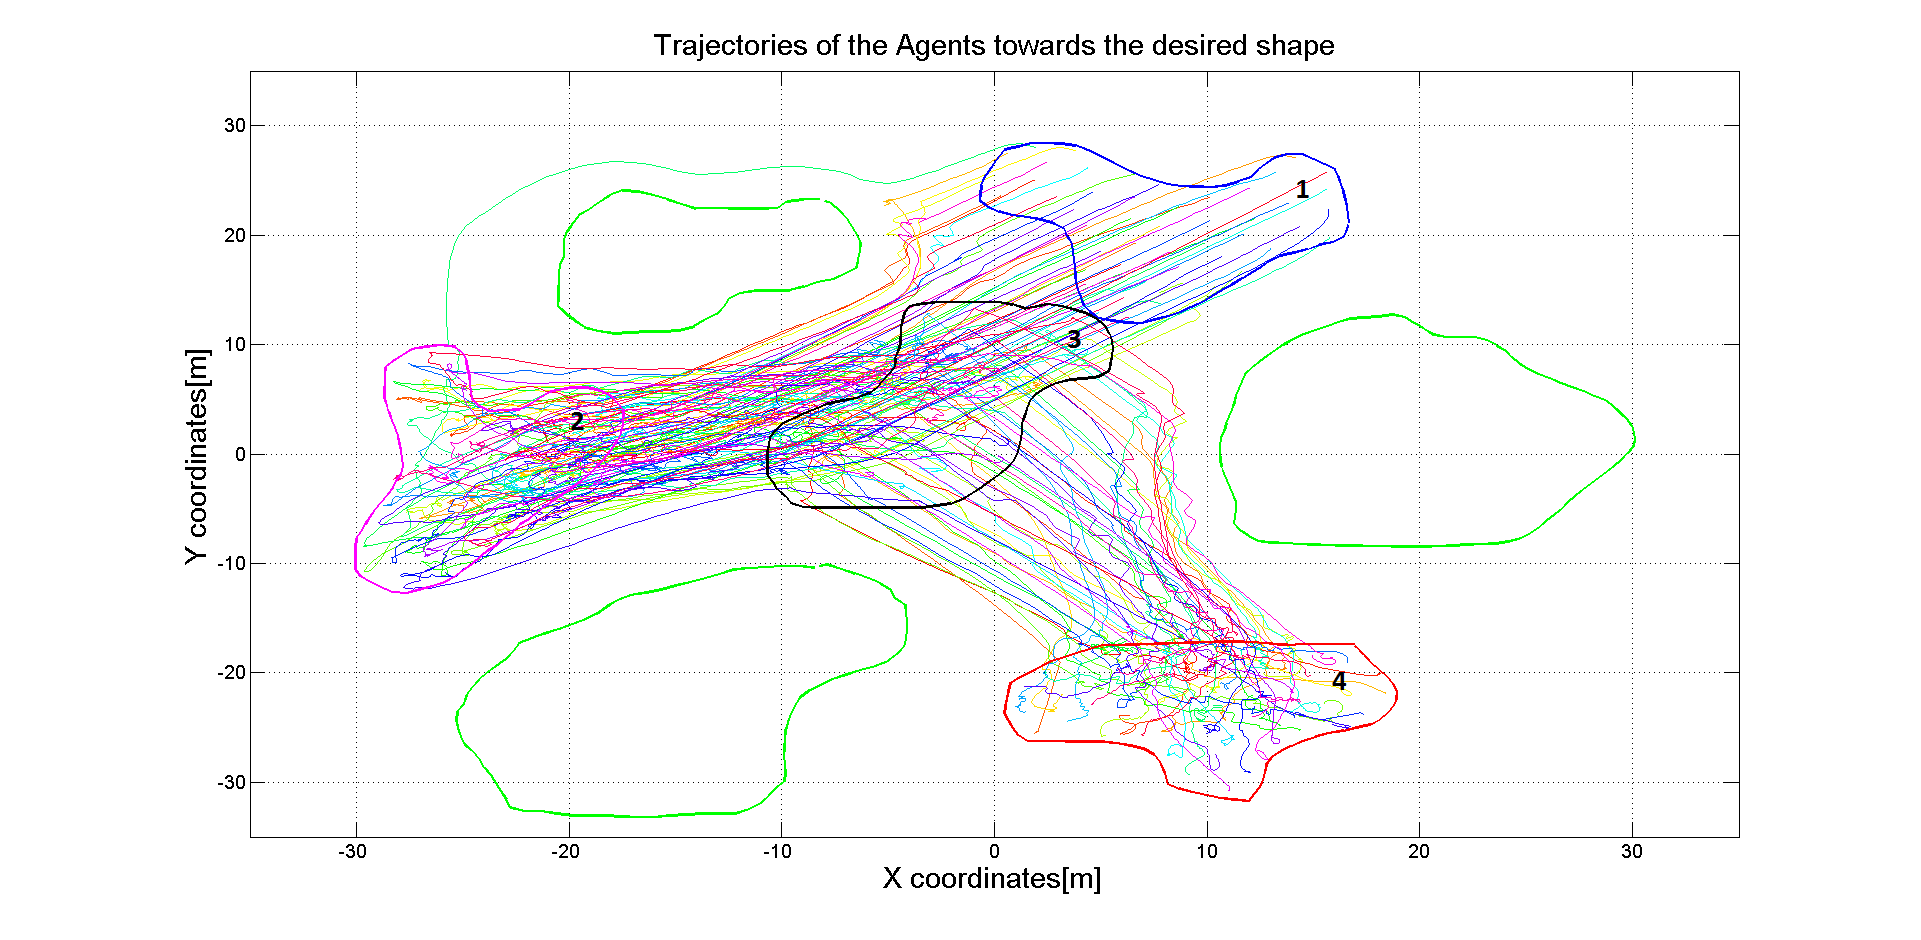
\includegraphics[scale = 0.33]{multiple_formation}}
\end{figure} 
		
\begin{center}
\captionof{table}{Performance Metrics for Multiple Formation Shapes} \label{perf_multiple} 
\begin{tabular}{|c|c|c|c|c|}
					
\hline
\textbf{} & \textbf{Total}  & \textbf{Total Settling} & \textbf{$\epsilon_t$} & \textbf{$\epsilon_g$} \\ \textbf{Method} & \textbf{Displacement[m]} & \textbf{Time[sec]}& \textbf{Mean} & \textbf{Mean} \\
\hline
Artificial&  &  &  & \\
 Forces & 4216 & 435& 2.21 & 0.68\\
 \hline
 Bubble&  &  &  & \\
 Packing &3876 &367 &2.31 & 0.56\\
\hline
 Randomized&  &  &  & \\
 Fractals &3769 &372 &3.35 & 1.16\\
\hline
\end{tabular}
\end{center}